%%%%%%%%%%%%%%%%%%%%%%%%%%%%%%%%%%%%%%%%%%%%%%%%%%%%%%%%%%%%%%
\chapter{Analysis strategy}\label{ch:strategy}
%%%%%%%%%%%%%%%%%%%%%%%%%%%%%%%%%%%%%%%%%%%%%%%%%%%%%%%%%%%%%%

This chapter describes in details the strategy followed in this search, that starting from the physics objects and identification algorithms described in the previous chapters, leads to the final results of the analysis.
Although preliminary selections on the objects expected in the final state have already been discussed, tighter requirements and a categorization of the events are applied as described in Section~\ref{sec:finalselection} to maximize the analysis sensitivity to the signals under study. The final discriminating observable used to search for the signal is the invariant mass of the diboson system. In fact, a possible signal would appear as a localized excess of data on the top of a smooth background. An accurate description of the expected background and signal distributions is therefore fundamental. A background estimation method for the main W+jets component, which makes use of data in sideband regions is used and described in Section~\ref{sec:alpha}. Another important source of background is represented by top quark production, which is estimated from data in a dedicated control region as discussed in Section~\ref{sec:ttbar}. The background model together with the signal model presented in Section~\ref{sec:signalModel} is used to perform a maximum likelihood fit of the data in the statistical analysis.
The systematic uncertainties in the signal and background predictions discussed in Section~\ref{sec:systUnc} are treated as nuisance parameters in the statistical interpretation.
Finally, Section~\ref{sec:stat} describes the standard procedure for the statistical test of the new signal hypothesis commonly used by LHC experiments and originally employed for the Higgs boson search.
The final results are presented in the next chapters.

%\section{Final event selection and categorization}\label{sec:finalselection}
 %%%%%%%%%
\section{Event selection and categorization}\label{sec:finalselection}
%%%%%%%%%

Events are selected online with triggers requiring either one muon or electron (Sections~\ref{subsec:eletrigger} and~\ref{subsec:mutrigger}).
Several requirements are then applied offline to the selected events to enhance the analysis sensitivity as described in the following.\\
%The strategy is slightly different for the two analyses described in this work and they will both summarized in the following.

The two analyses described in this work feature the same selection strategy on the leptonic part of the final state.
Both analyses require exactly one muon or one electron satisfying certain \pt and $\eta$ requirements and passing 
the high-\pt lepton identification criteria described in Sections~\ref{subsec:muonid} and~\ref{subsec:eleid}.
As summarized in Tables~\ref{tab:cutsummaryWH} and~\ref{tab:cutsummaryWV}, the only difference is in the \pt threshold of the lepton which is higher for the 13\TeV data analysis
to match the increase in the trigger threshold. The offline reconstructed \pt of the electron must be greater than 90 (120)\GeV for the 8 (13)\TeV data analysis, where the trigger reaches the plateau.
This is required in order to avoid any bias on the distributions due to the turn-on of the trigger efficiency curve and its description in simulation.
%In fact, this choice is made to simplify the analysis avoiding the need for modelling possible biases in the distributions due to the turn-on of the trigger efficiency curve.
%In fact, this choice is made to simplify the analysis avoiding the need for modelling the turn-on of the trigger efficiency curve and, as a consequence, reducing the associated systematic uncertainties.
Reconstructed electrons must have $|\eta| < 2.5$ and also be located outside of the overlap region between the ECAL barrel and endcaps, because the reconstruction of an electron object in
this region is not optimal. In a similar way, the offline reconstructed \pt of the muon must be greater than 50 (53)\GeV for the 8 (13)\TeV analysis, and within $|\eta| < 2.1$ as a consequence of the trigger criteria.
Events with additional well-identified muons and/or electrons are rejected to avoid contamination from events containing $\PZ\to\ell\ell$ decays.\\

\begin{table}[!htb]
\begin{center}
\caption{Summary of the final selection for the 8\TeV data analysis in the $\ell\nu\bbbar$ final state.}
\label{tab:cutsummaryWH}
\begin{tabular}{lc}
\hline
\multicolumn{1}{c}{\textbf{Selection}} & \textbf{Value}\\
\hline
\multicolumn{1}{c}{Lepton selection}\\
\cline{1-1}
Electron & $\pt > 90\GeV$\\
              & $|\eta| < 2.5$ except [1.44, 1.57] range\\
Muon    & $\pt > 50\GeV$\\
             & $|\eta|<2.1$\\
\hline
\multicolumn{1}{c}{AK5 jet selections}\\
\cline{1-1}
Jet \pt &  $\pt >30\GeV$\\
Jet $\eta$  & $|\eta|<2.4$\\
\hline
\multicolumn{1}{c}{\ETmiss selections}\\
\cline{1-1}
\ETmiss (electron channel) &  \ETmiss$>80~\GeV$\\
\ETmiss (muon channel) & \ETmiss$>40~\GeV$\\
\hline
\multicolumn{1}{c}{Boson selections}\\
\cline{1-1}
$\PW\to\ell\Pgn$ & $\pt > 200\GeV$\\
$\PH\to\bbbar$ (CA8 jet) & $\pt > 200\GeV$\\
 & $|\eta| < 2.4$ except [1.0, 1.8] range\\
Back-to-back topology & $\Delta R (\ell , \PH_{\bbbar}) > \pi/2$ $\,$\\
                      & $\Delta \phi (\PH_{\bbbar} , \ptvecmiss)>2$\\ 
                      & $\Delta \phi (\PH_{\bbbar} , \PW_{\ell\Pgn})>2$\\
Diboson invariant mass & $\mWH > 0.7\TeV$\\                      
\hline
\multicolumn{1}{c}{H tagging selections}\\
\cline{1-1}
Pruned jet mass       & $110 < \mJ < 135\GeV$\\
Combined b-tagging cut	& 2 CSVL b-tagged subjets if $\Delta R(\mathrm{subjets}) > 0.3$\\
			& 1 CSVL b-tagged CA8 jet if $\Delta R(\mathrm{subjets})$\\ 
\hline
\multicolumn{1}{c}{\ttbar rejection}\\
\cline{1-1}
B-tag veto      & no CSVM b-tagged AK5 jet\\
		& within $\Delta R (\PH_{\bbbar}, AK5) = 0.8$\\
Top quark mass veto	& $m_\mathrm{top}^\mathrm{l} < 120~||~m_\mathrm{top}^\mathrm{l} > 240$\\
		& $m_\mathrm{top}^\mathrm{h} < 160~||~m_\mathrm{top}^\mathrm{h} > 280$\\
\hline
\end{tabular}
\end{center}
\end{table}

\begin{table}[!htb]
\begin{center}
\caption{Summary of the final selection for the 13\TeV data analysis in the $\ell\nu\qqbar$ final state.}
\label{tab:cutsummaryWV}
\begin{tabular}{lc}
\hline
\multicolumn{1}{c}{\textbf{Selection}} & \textbf{Value}\\
\hline
\multicolumn{1}{c}{Lepton selection}\\
\cline{1-1}
Electron & $\pt > 120\GeV$\\
              & $|\eta| < 2.5$ except [1.44, 1.57] range\\
Muon    & $\pt > 53\GeV$\\
             & $|\eta|<2.1$\\
\hline
\multicolumn{1}{c}{AK4 jet selections}\\
\cline{1-1}
Jet \pt &  $\pt >30\GeV$\\
Jet $\eta$  & $|\eta|<2.4$\\
\hline
\multicolumn{1}{c}{\ETmiss selections}\\
\cline{1-1}
\ETmiss (electron channel) &  \ETmiss$>80~\GeV$\\
\ETmiss (muon channel) & \ETmiss$>40~\GeV$\\
\hline
\multicolumn{1}{c}{Boson selections}\\
\cline{1-1}
$\PW\to\ell\Pgn$ & $\pt > 200\GeV$\\
$\PV\to\qqbar$ (AK8 jet) & $\pt > 200\GeV$\\
 & $|\eta| < 2.4$\\
Back-to-back topology & $\Delta R (\ell , \PV_{\qqbar}) > \pi/2$ $\,$\\
                      & $\Delta \phi (\PV_{\qqbar} , \ptvecmiss)>2$\\ 
                      & $\Delta \phi (\PV_{\qqbar} , \PW_{\ell\Pgn})>2$\\
Diboson invariant mass & $\mWV > 0.7\TeV$\\                       
\hline
\multicolumn{1}{c}{V tagging selections}\\
\cline{1-1}
Pruned jet mass       & $ 65 < \mJ < 105\GeV$\\
2- to 1-subjettiness ratio & $\nsubj <$ 0.6\\
\hline
\multicolumn{1}{c}{\mJ categories}\\
\cline{1-1}
WW-enriched   & $ 65 < \mJ < 85\GeV$ \\
WZ-enriched   & $ 85 < \mJ < 105\GeV$\\
\hline
\multicolumn{1}{c}{\ttbar rejection}\\
\cline{1-1}
B-tag veto      & no CSVM b-tagged AK5 jet\\
		& within $\Delta R (\PV_{\qqbar}, AK5) = 0.8$\\				       
\end{tabular}
\end{center}
\end{table}

The requirements \ETmiss $>$ 40 and $>$ 80\GeV are applied, respectively, in the muon and electron channels.
The threshold is higher in the electron channel to further suppress the larger background from multijet processes expected at low values of \ETmiss due to jets misidentified as electrons.
This background is expected to be negligible in the muon channel, for which a lower \ETmiss threshold can be used to preserve a higher efficiency for a low-mass signal.
The identified lepton and the \ETmiss are used to reconstruct the W $\rightarrow\ell\Pgn$ candidate as described in Section~\ref{sec:leptonicW},
which is required to have $\pt > 200\GeV$.\\

A different strategy is instead used in the two analyses, for the hadronic part of the final state.
As described in Section~\ref{sec:jets}, the CA8 and AK8 algorithms are used to reconstruct the H and V jet candidates in the 8 and 13\TeV analysis, respectively.
In both cases the jet is required to have $\pt > 200\GeV$ and $|\eta| < 2.4$. %In addition, jets within $\Delta R < 0.8$ of any well-identified electron or muon are not used in the analysis.
For CA8 jets, the pseudorapidity region $1.0 < |\eta| < 1.8$ is excluded corresponding to the barrel-endcap transition region of the silicon tracker where the reconstruction of tracks is not optimal (Section~\ref{subsec:jetsreco}).
The probability of signal events with jets outside this region is 80\% (92\%) for a resonance mass of 1.0 (2.5)\TeV.

The 8\TeV analysis aims at isolating events with a high-\pt Higgs boson decaying to \bbbar and the H tagging algorithm described in Section~\ref{sec:htagging} is applied.
The H tagging requires the selected CA8 jet to have pruned mass in the range $110 < \mJ < 135\GeV$. Furthermore, the subjets are required to be b-tagged with the CSVL algorithm if their angular distance $\Delta R < 0.3$.
Otherwise, b tagging is applied to the whole CA8 jet using the same algorithm.

The 13\TeV analysis is instead focused on events with a high-\pt V boson decaying to \qqbar and the V tagging algorithm described in Section~\ref{sec:htagging} is applied in this case.
The pruned jet mass window is shifted down to the V boson mass, requiring the selected AK8 jet to have pruned mass in the range $65 < \mJ < 105\GeV$.
Furthermore, the V jet is required to have $\nsubj < 0.6$.
Finally, the V jet is deemed a W-boson candidate if its pruned mass falls in the range 65--85\GeV, while it is deemed a Z-boson candidate if it falls in the range 85--105\GeV instead.
This categorization has been added on the top of the V tagging requirements on the \mJ to enhance discrimination between resonances with different charge and spin. 
Indeed, the first category, referred to as  ``WW-enriched'', has a higher sensitivity for resonances such as the neutral spin-2 graviton or the neutral spin-1 \Zpr decaying to WW, where a W jet is expected.
The second category, referred to as ``WZ-enriched'', is instead optimized for resonances such as the charged spin-1 \Wpr decaying to WZ, where a Z jet is expected.\\

In addition, there are specific topological selection criteria chosen for both the analyses. 
It is required that the two V bosons from the decay of a massive resonance are approximately back-to-back:
the $\Delta R$ between the lepton and the signal jet is greater than $\pi/2$; the $\Delta\phi$ between the vector \ptvecmiss and the signal jet,
as well as between the $\PW\to\ell\Pgn$ and signal jet candidates, are both greater than 2 radians.

To reduce the level of the \ttbar background, events with one or more reconstructed AK5 (or AK4) jets, not overlapping with the signal jet candidate are analyzed:
if one or more of these jets is b-tagged with the CSVM algorithm, the event is rejected.
For the 8\TeV analysis additional selections are applied to further reduce contamination from \ttbar background.
In fact, the b tagging requirements in this analysis enhance the contribution from top quark production where real b jets are present.
A leptonically decaying top quark candidate mass $m_\mathrm{top}^\mathrm{l}$ is reconstructed from the lepton, \ETmiss, and the closest AK5 jet to the lepton using the method described in Section~\ref{sec:leptonicW}.
A hadronically decaying top quark candidate mass $m_\mathrm{top}^\mathrm{h}$ is also reconstructed, from the H jet candidate and the closest AK5 jet.
Events with $120 < m_\mathrm{top}^\mathrm{l} < 240\GeV$ or $160 < m_\mathrm{top}^\mathrm{h} < 280\GeV$ are rejected.
The chosen windows around the top quark mass are the result of an optimization carried out in this analysis, taking into account
the asymmetric tails at larger values due to combinatorial background.\\

According to the above description of the final selections, the event categorization is based on 2 orthogonal classes of events for the 8\TeV data analysis in the $\ell\nu\bbbar$ final state,
depending on the lepton flavour (muon or electron),
and on 4 orthogonal classes of events for the 13\TeV data analysis in the $\ell\nu\qqbar$ final state, depending on the lepton flavour and on the pruned jet mass category (WW or WZ).

The two boson candidates are combined into a diboson candidate, with presence of signal then inferred from the observation of localized excesses in the $\mlvj$ distribution.
When several diboson resonance candidates are present in the same event, only the one with the highest \pt
V or H jet is kept for further analysis.

The reconstructed invariant mass of the resonance is required to be at least 0.7\TeV.\\ 

The distributions in \pt and N-subjettiness ratio \nsubj distributions for the V jet candidate in the $\ell\Pgn\qqbar$ channel is shown in Fig.~\ref{fig:controlPlots13TeV},
after requiring $65 < \mJ < 105\GeV$, for both simulation and 13\TeV data.  Figure~\ref{fig:controlPlots8TeV} shows the distribution in \pt for the H jet candidate
after requiring $40 < \mJ < 110\GeV$, for both simulation and 8\TeV data.

\begin{figure}[!htb]
\centering
\subfigure[]{\label{fig:controlPlots13TeV_a}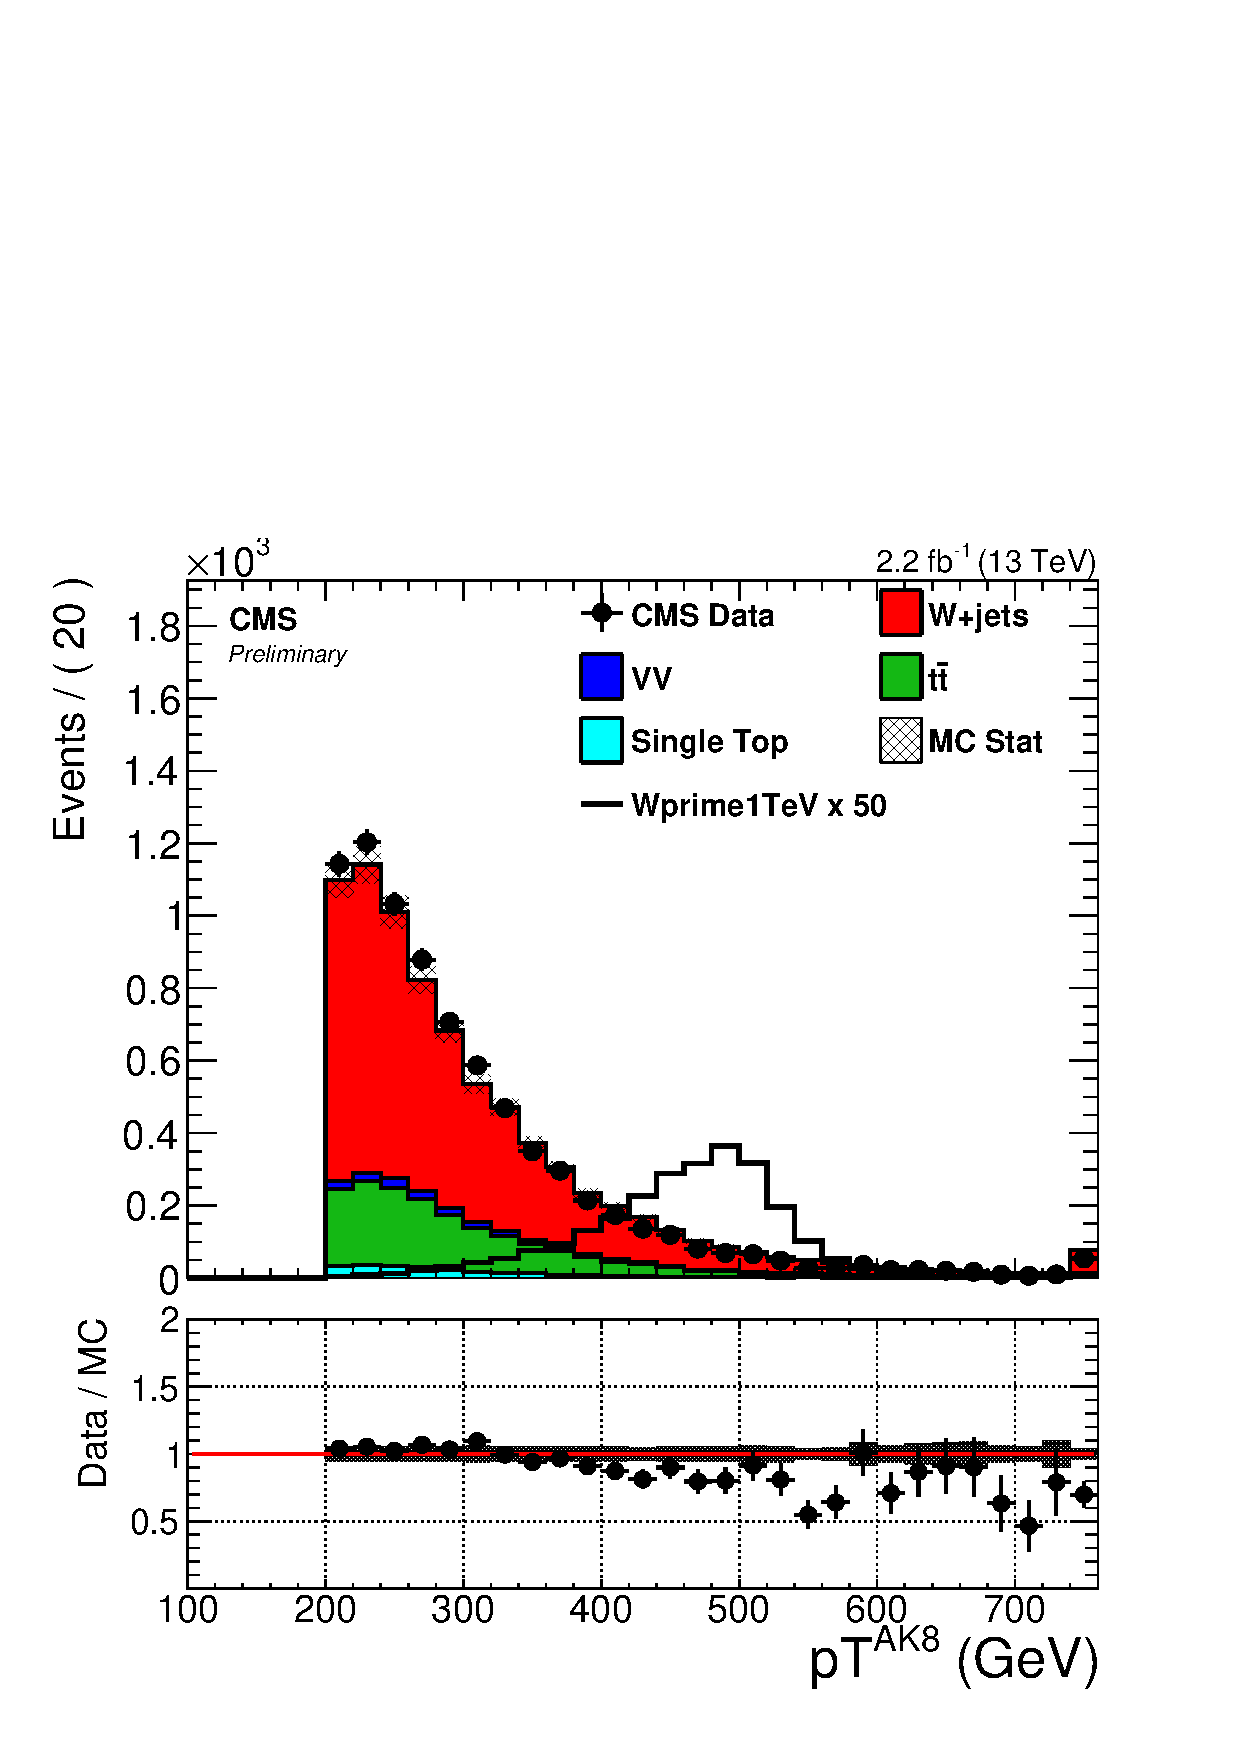
\includegraphics[width=0.45\textwidth]{\cheight/ptvjet-13TeV-wjets.pdf}}
\subfigure[]{\label{fig:controlPlots13TeV_b}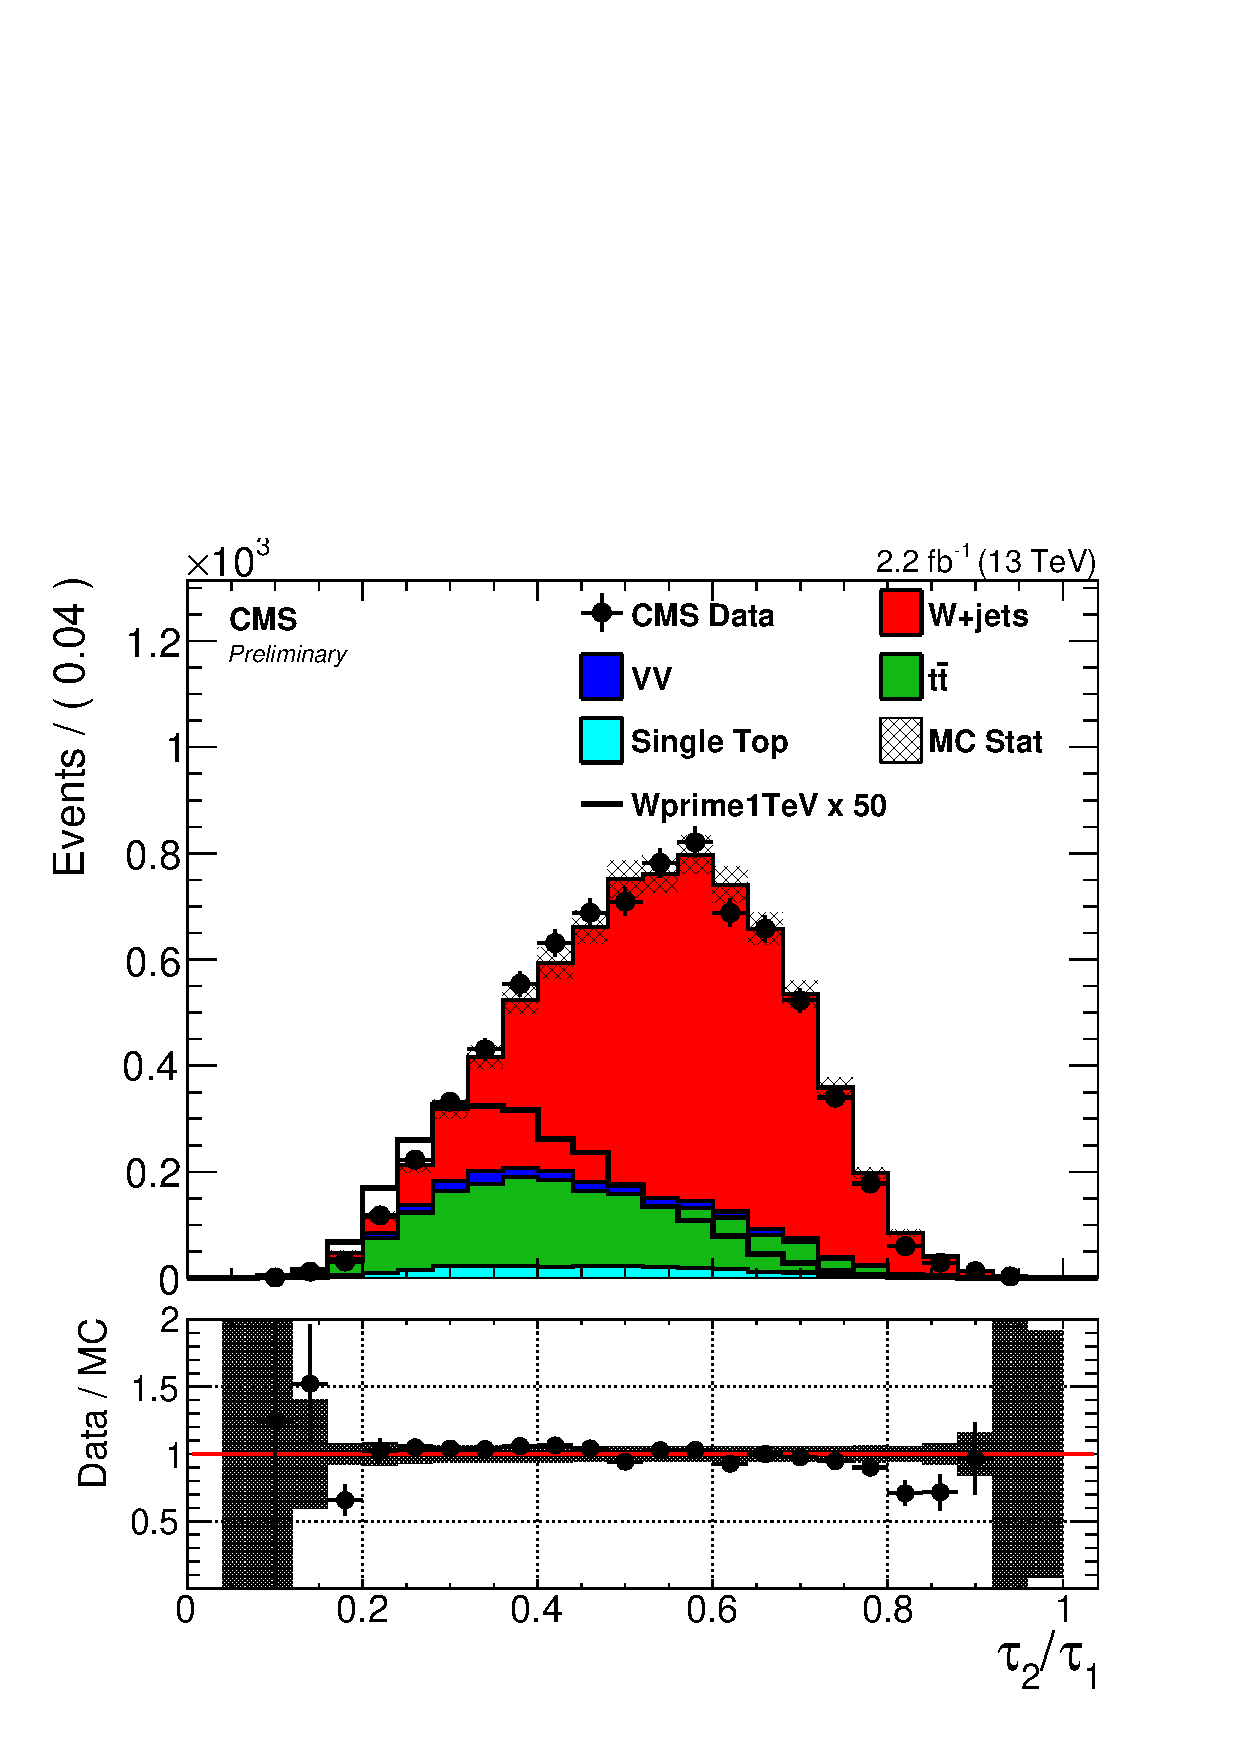
\includegraphics[width=0.45\textwidth]{\cheight/tau21-13TeV-wjets.pdf}}
\caption{Distributions in \pt (a) and N-subjettiness ratio \nsubj (b) for the V jet candidate obtained requiring $65 < \mJ < 105\GeV$ after merging muon and electron channels. The SM diboson, \ttbar, and single top quark backgrounds are taken from simulation and are normalized to the integrated luminosity of the 13\TeV data sample. The W+jets background is rescaled to match the number of events in data.}
\label{fig:controlPlots13TeV}
\end{figure}

\begin{figure}[!htb]
\centering
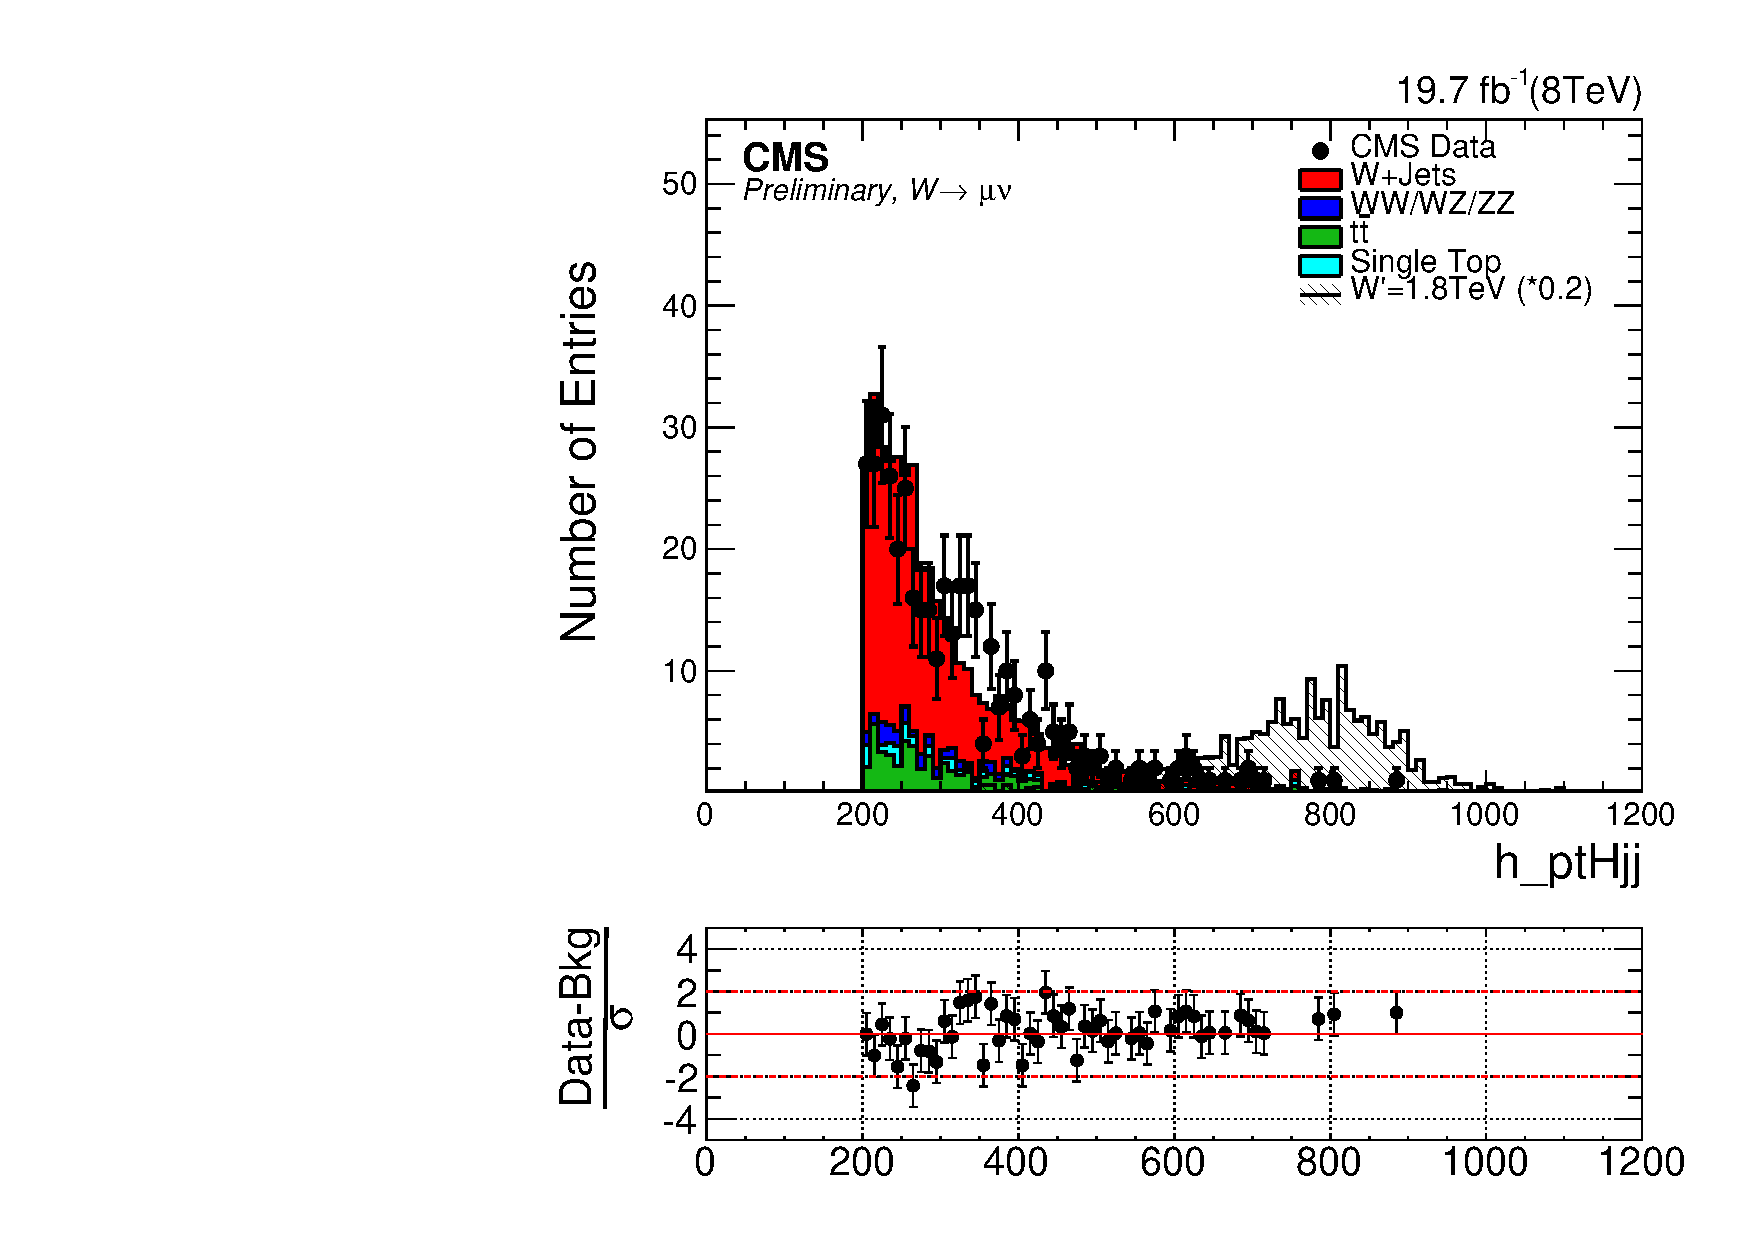
\includegraphics[width=0.5\textwidth]{\cheight/can_h_ptHjj.pdf}
\caption{Distributions in \pt for the H jet candidate obtained requiring $40 < \mJ < 110\GeV$ for events in the muon channel. The SM diboson, \ttbar, and single top quark backgrounds are taken from simulation and are normalized to the integrated luminosity of the 8\TeV data sample. The W+jets background is rescaled to match the number of events in data.}
\label{fig:controlPlots8TeV}
\end{figure}
  
 %\section{W+jets background estimate with $\alpha$ ratio method}\label{sec:alpha}
 %%%%%%%%%
\section{W+jets background estimate with $\alpha$ ratio method}\label{sec:alpha}
%%%%%%%%%

The $\mlvj$ distribution observed in data is dominated by SM background processes where single
quark or gluon jets are falsely identified as W or H jets. The dominant process is inclusive W boson production. 
Since both normalization and shape discrepancies are visibile between data and simulation (Figures~\ref{fig:controlPlots13TeV} and~\ref{fig:controlPlots8TeV}),
a data driven method has been developed to estimate this background component, as described in the following.
Sub-dominant backgrounds include \ttbar, single top quark, and non resonant diboson SM production,
which are estimated from simulation, after applying correction factors for residual data-to-simulation disagreement measured in control samples selected in data.

\subsection{Background estimation procedure}

The W+jets background is estimated through the so called \textit{$\alpha$ ratio} method.
This method assumes that the correlation between \mJ and $\mlvj$ for the dominant W+jets background can be adequately modelled by simulation.
A signal-depleted control region (sideband) is defined by requiring the mass of the V or H jet to lie below or above the nominal selection; the
$\mlvj$ distribution observed in this region is then extrapolated to the nominal region through
a transfer function estimated from simulation. Other minor sources of background, such as
\ttbar, single top quark, and SM diboson production, are estimated using simulated events after
applying correction factors based on control regions in data, as described in Sections~\ref{sec:vtagging} and~\ref{sec:ttbar}.
The sideband region is defined around the jet mass window that represents the analysis signal region (Section~\ref{sec:finalselection}).
The lower and upper sidebands for the two analyses are summarized in Table~\ref{tab:sidebands}.
For the 13\TeV analysis a ``gap'' is introduced between the signal region and the upper sideband, since the
range defined by $105 < \mJ < 135$ might include contribution from signals with highly Lorentz-boosted Higgs bosons in the final state.
Since these types of searches at 13\TeV~\cite{Khachatryan:2016cfx} have been performed simultaneously with the one described in this work,
this region has been discarded to avoid introducing a bias in the shape and normalization extrapolation due to a possible signal.
On the other hand, the lower sideband of the 8\TeV $\ell\Pgn\bbbar$ analysis includes the region where signals from highly Lorentz-boosted V bosons might occur.
In fact, this analysis has been performed after the search for WV resonances in the lepton+jet final state at 8\TeV disclosed the signal region,
where no deviation from the predicted SM background have been observed~\cite{Khachatryan:2014gha}.

\begin{table}[!htb]
\centering
\caption{Sideband regions used in the two analyses to estimate the contribution from the main W+jets background.}
\begin{tabular}{lcc}
\multirow{2}{*}{{\bf \mJ sideband}} &\multicolumn{2}{c}{{\bf Decay channel}}\\
 & $\ell\Pgn\bbbar$& $\ell\Pgn\qqbar$\\
\hline
\hline
Low sideband (LSB) & 40--110\GeV & 40--65\GeV\\ 
High sideband (HSB) & 135--150\GeV & 135--150\GeV\\ 
\end{tabular}
\label{tab:sidebands}
\end{table}

\subsection{Extraction of the W+jets normalization}

The overall normalization of the W+jets background in the signal region is determined from a
fit to the \mJ distribution in the lower and upper sidebands of the data. The analytical form
of the fitting function is chosen from simulation studies, as are the contributions from minor backgrounds. 
%Figure 3 shows the result of this fit for the low- and high-mass `n+jet channels.
A summary of the empirical functional forms used to parametrize each background contribution are listed in Table~\ref{tab:mjfunct}, and defined as follows:

\footnotesize
\begin{equation}
\begin{gathered}
   F_{\rm Exp}(x)=e^{cx}\\
   F_{\rm ErfExp}(x)=e^{cx} \cdot \frac{1 + {\rm Erf}((x-a)/b)}{2} \\
   F_{\rm ExpGaus}(x) = c_{0} \cdot e^{cx} + c_{1} \cdot \mathrm{Gaus}(x,x_{1},\sigma_{1})\\
   F_{\rm 4Gaus}(x) = c_{1} \cdot \mathrm{Gaus}(x,x_{1},\sigma_{1}) + c_{2} \cdot \mathrm{Gaus}(x,x_{2},\sigma_{2}) + c_{3} \cdot \mathrm{Gaus}(x,x_{3},\sigma_{3}) + c_{4} \cdot \mathrm{Gaus}(x,x_{4},\sigma_{4}) \\
   F_{\rm ErfExp2Gaus}(x) = e^{cx} \cdot \frac{1 + {\rm Erf}((x-a)/b)}{2} + c_{1} \cdot \mathrm{Gaus}(x,x_{1},\sigma_{1}) + c_{2}\cdot \mathrm{Gaus}(x,x_{2},\sigma_{2})\\
\end{gathered}
\label{eqn:mjfunct}
\end{equation}

\normalsize
\begin{table}[!htb]
\centering
\caption{Summary of the empirical functional forms used to fit the \mJ spectra of each background component in the two analyses.}
\begin{tabular}{lcccc}
Decay channel & W+jets & \ttbar & Single top quark & Diboson\\
\hline
\hline
$\ell\Pgn\bbbar$ & $F_{\rm ErfExp}(x)$ & $F_{\rm Exp}(x)$ & $F_{\rm Exp}(x)$ & $F_{\rm ExpGaus}(x)$\\
$\ell\Pgn\qqbar$ & $F_{\rm ErfExp}(x)$ & $F_{\rm ErfExp2Gaus}(x)$ & $F_{\rm ExpGaus}(x)$ & $F_{\rm 4Gaus}(x)$
\end{tabular}
\label{tab:mjfunct}
\end{table}

Figure~\ref{fig:mcfits_mj} shows the functional forms listed in Table~\ref{tab:mjfunct} for the $\ell\Pgn\qqbar$ channel, after fitting the simulation data of each background component,
demonstrating that the chosen functions well reproduce the expected \mJ spectra.

\begin{figure}[!htb]
\centering
\subfigure[]{\label{fig:mcfits_mj_a}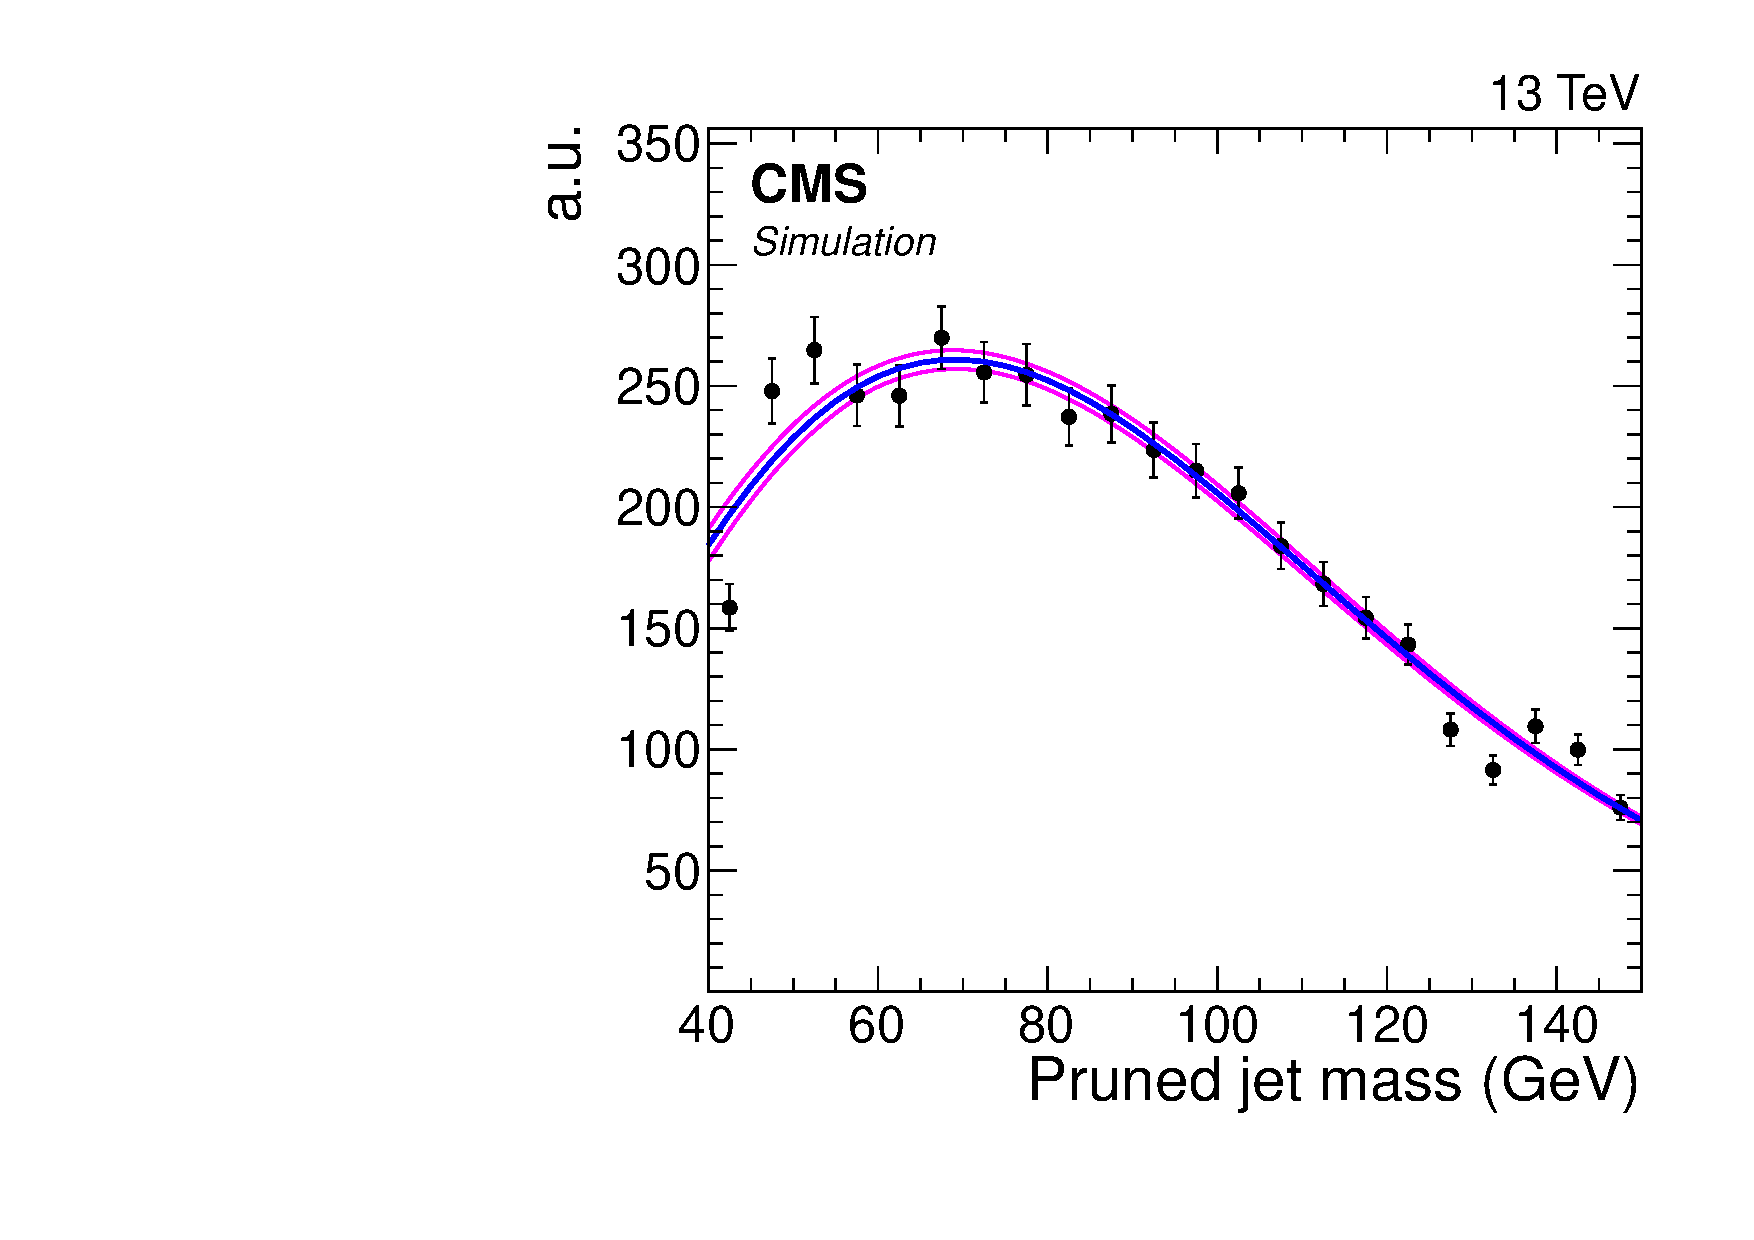
\includegraphics[width=0.45\textwidth]{\cheight/HP_mj_fitting-mu-WJets.pdf}}
\subfigure[]{\label{fig:mcfits_mj_b}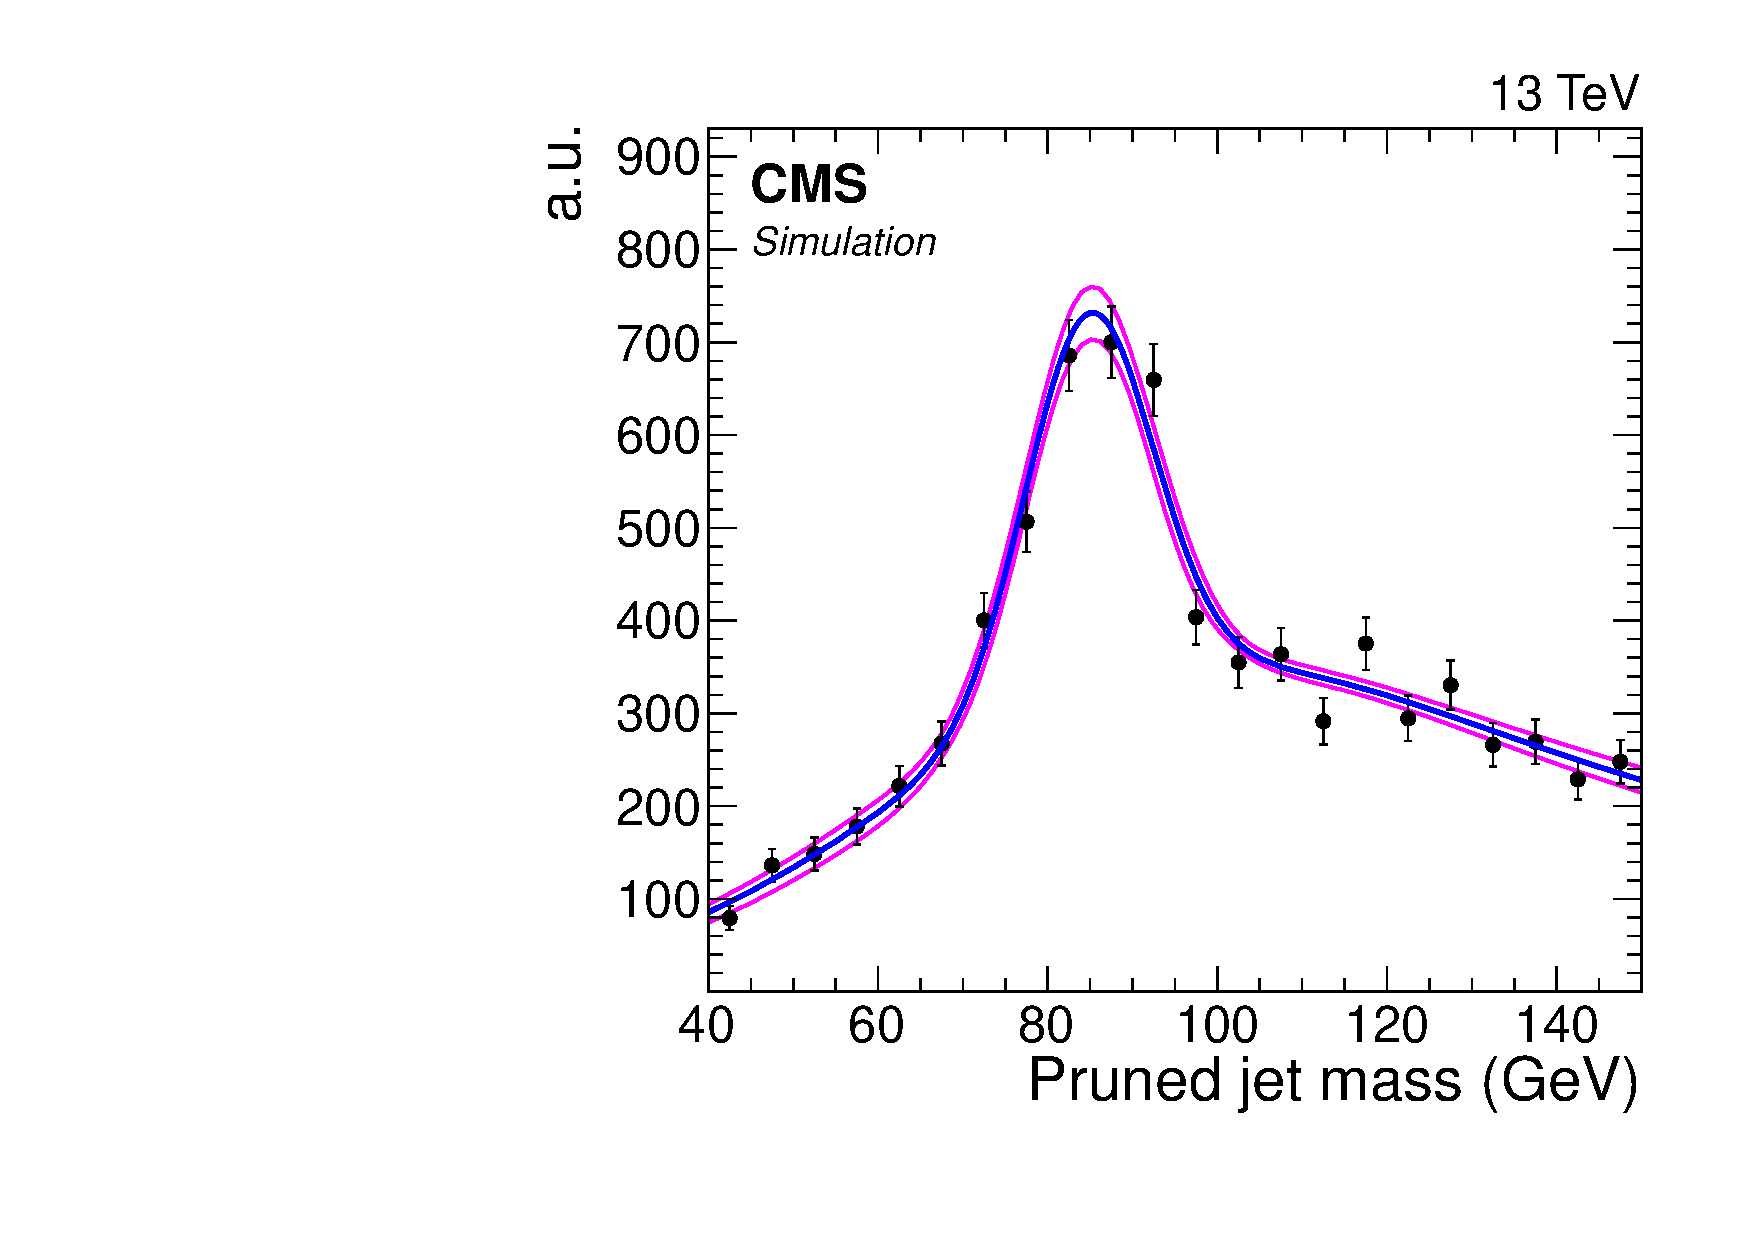
\includegraphics[width=0.45\textwidth]{\cheight/HP_mj_fitting-mu-TTbar.pdf}}\\
\subfigure[]{\label{fig:mcfits_mj_c}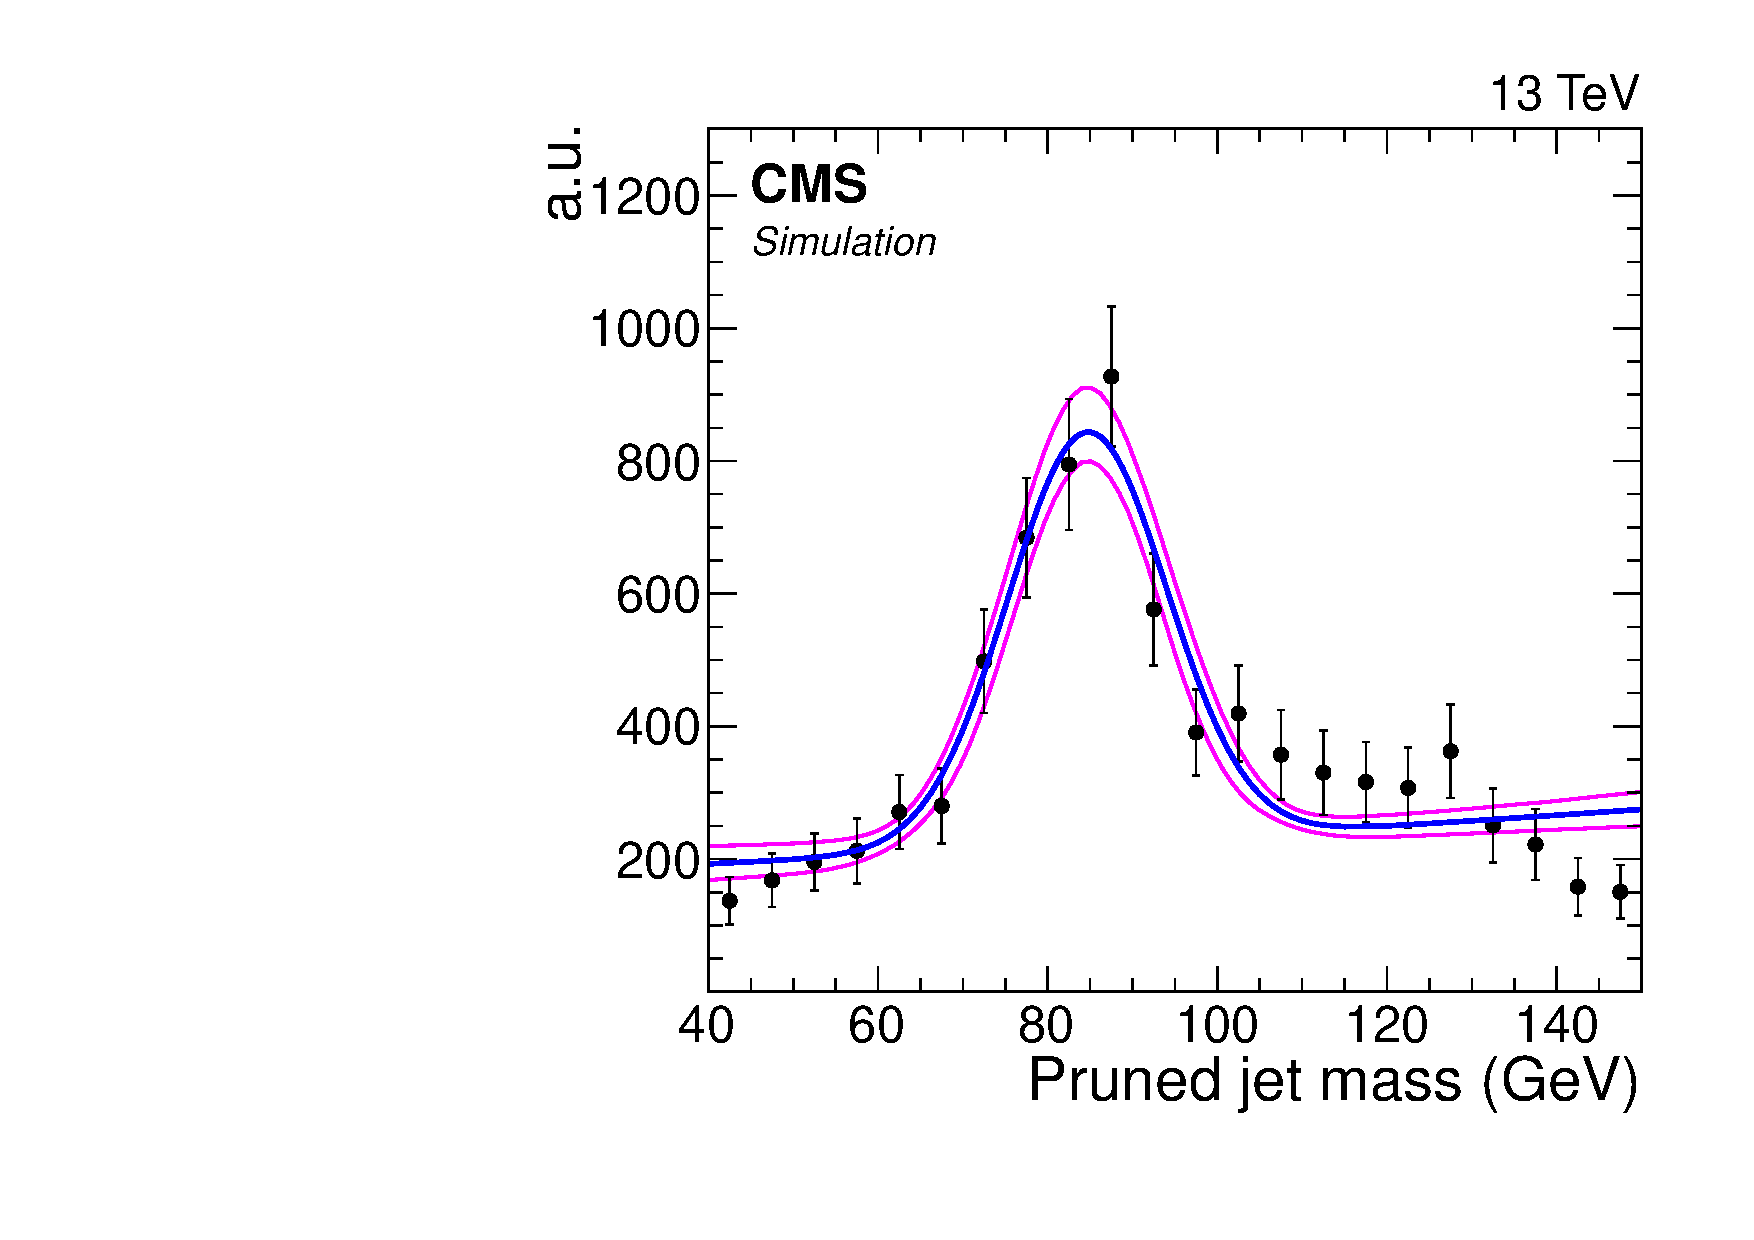
\includegraphics[width=0.45\textwidth]{\cheight/HP_mj_fitting-mu-STop.pdf}}
\subfigure[]{\label{fig:mcfits_mj_d}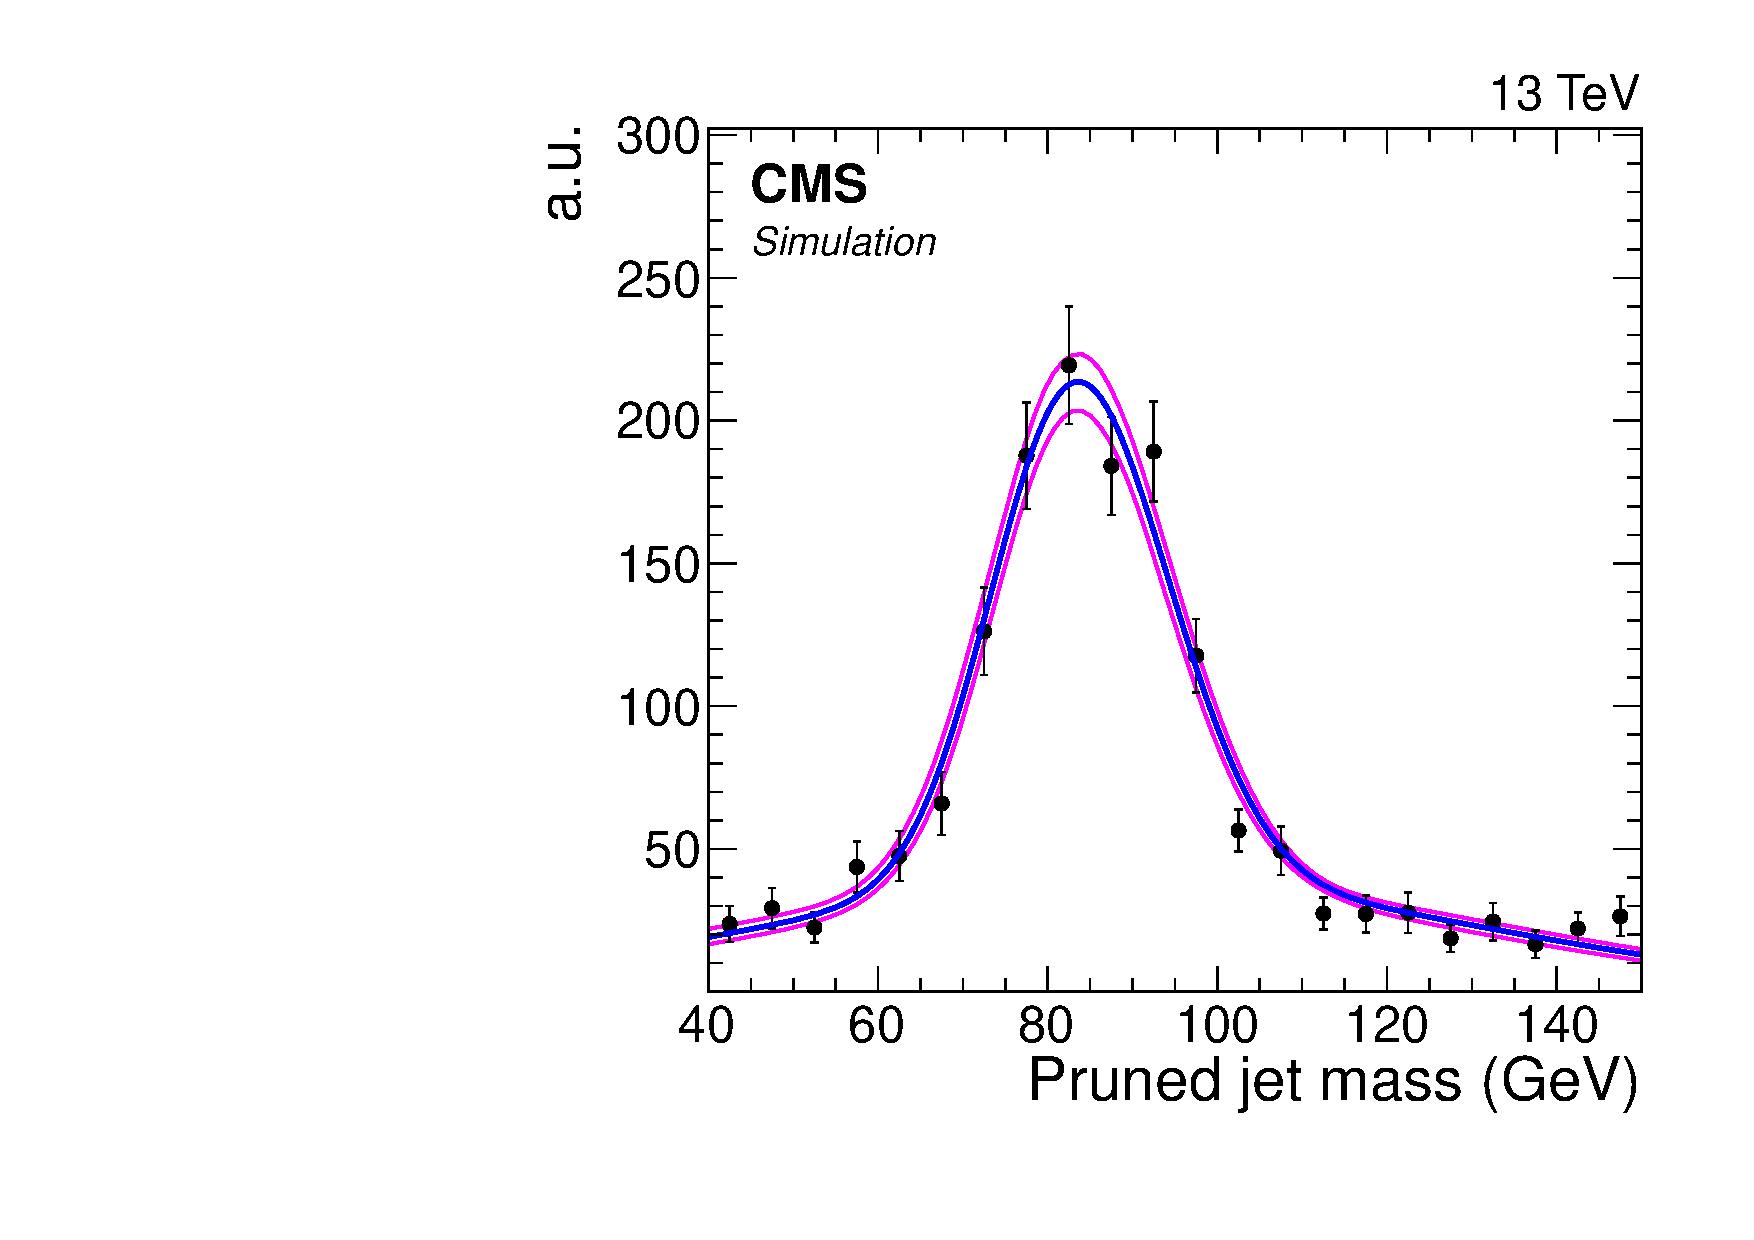
\includegraphics[width=0.45\textwidth]{\cheight/HP_mj_fitting-mu-VV.pdf}}
\caption{Functional forms describing the \mJ spectra for each background contribution after fitting the simulation data. (a) W+jets. (b) \ttbar. (c) Single top quark. (d) Diboson.}
\label{fig:mcfits_mj}
\end{figure}

The results of this fit procedure to extract the W+jets normalization are shown in Fig.~\ref{fig:mjfit8TeV} and~\ref{fig:mjfit13TeV}
for the $\ell\Pgn\bbbar$ and the $\ell\Pgn\qqbar$ channel, respectively.
The factors for correcting the simulated W-peak position and resolution to represent the observed data, taken from the top quark enriched control sample as described in Section~\ref{sec:vtagging}, are included in the \mJ spectra of Fig.~\ref{fig:mjfit13TeV}. 

\begin{figure}[!htb]
\centering     %%% not \center
\subfigure[]{\label{fig:mjfit8TeV_a}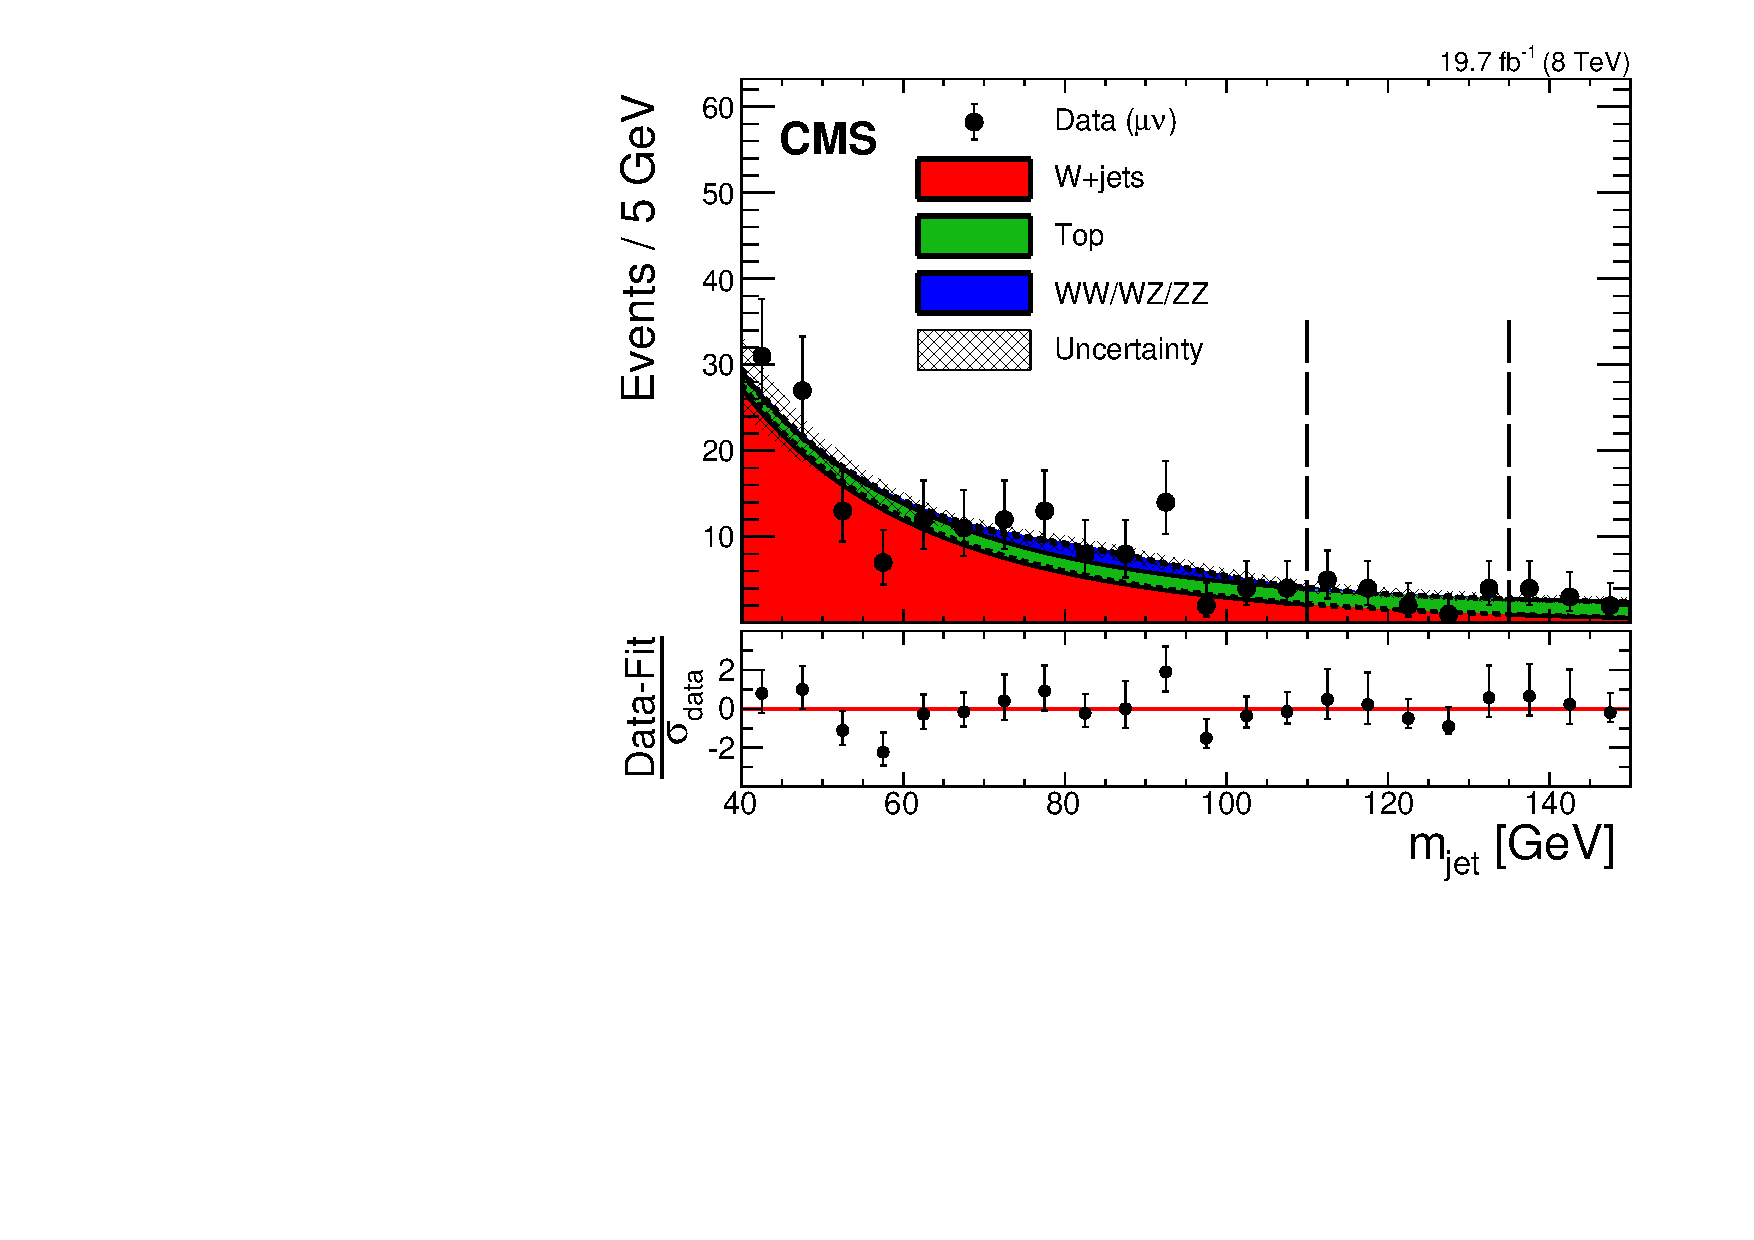
\includegraphics[width=0.45\textwidth]{\cheight/m_j_sideband_WJets0_MU_ALLP.pdf}}
\subfigure[]{\label{fig:mjfit8TeV_b}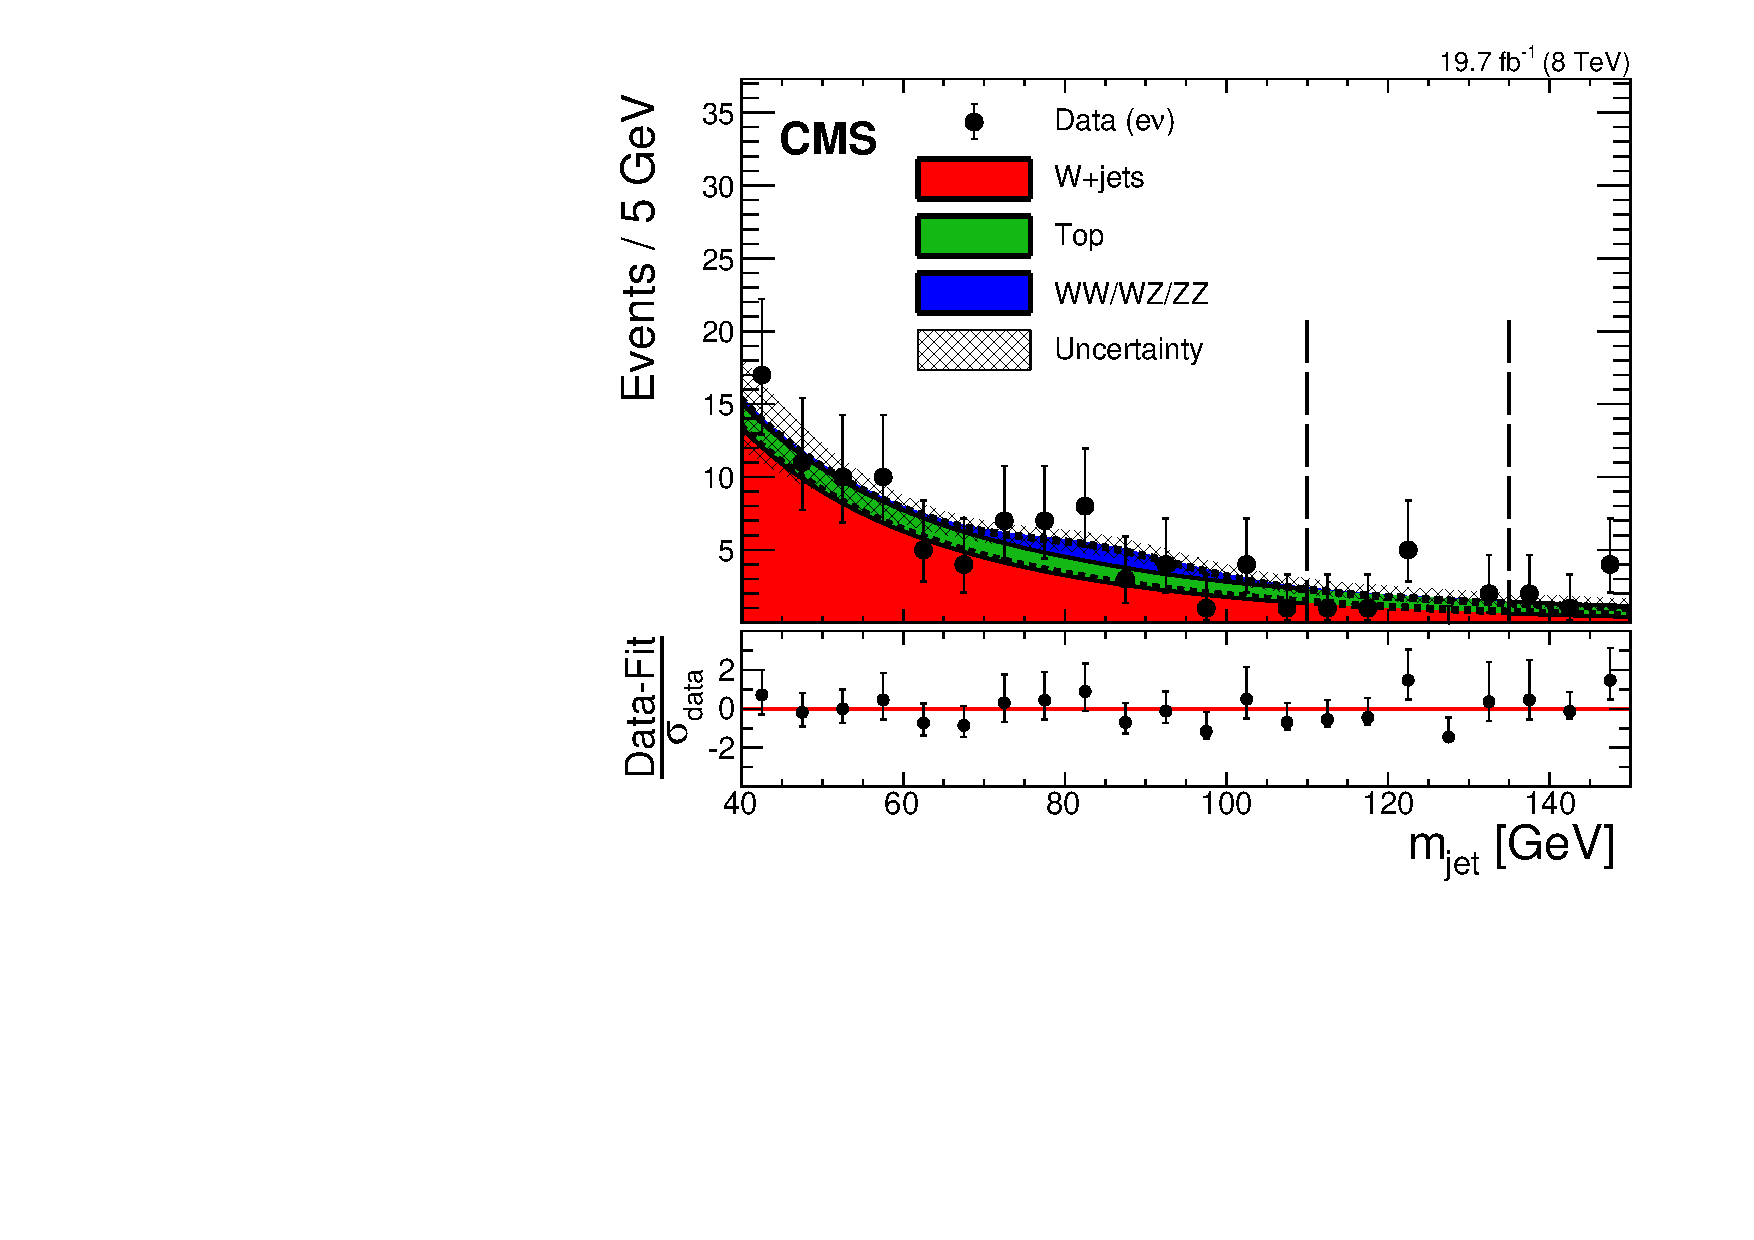
\includegraphics[width=0.45\textwidth]{\cheight/m_j_sideband_WJets0_ELE_ALLP.pdf}}
\caption{Distributions in pruned jet mass \mJ in the muon (a) and electron (b) channels for the $\ell\Pgn\bbbar$ analysis at 8\TeV. All selections are applied except the requirement on the \mJ signal window. The signal region lies between the dashed vertical lines. The hatched region indicates the statistical uncertainty of the fit. At the bottom of each plot, the bin-by-bin fit residuals, ($N_{\rm data}$ - $N_{\rm fit}$)/$\sigma_{\rm data}$, are shown.}
\label{fig:mjfit8TeV}
\end{figure}

\begin{figure}[!htb]
\centering     %%% not \center
\subfigure[]{\label{fig:mjfit13TeV_a}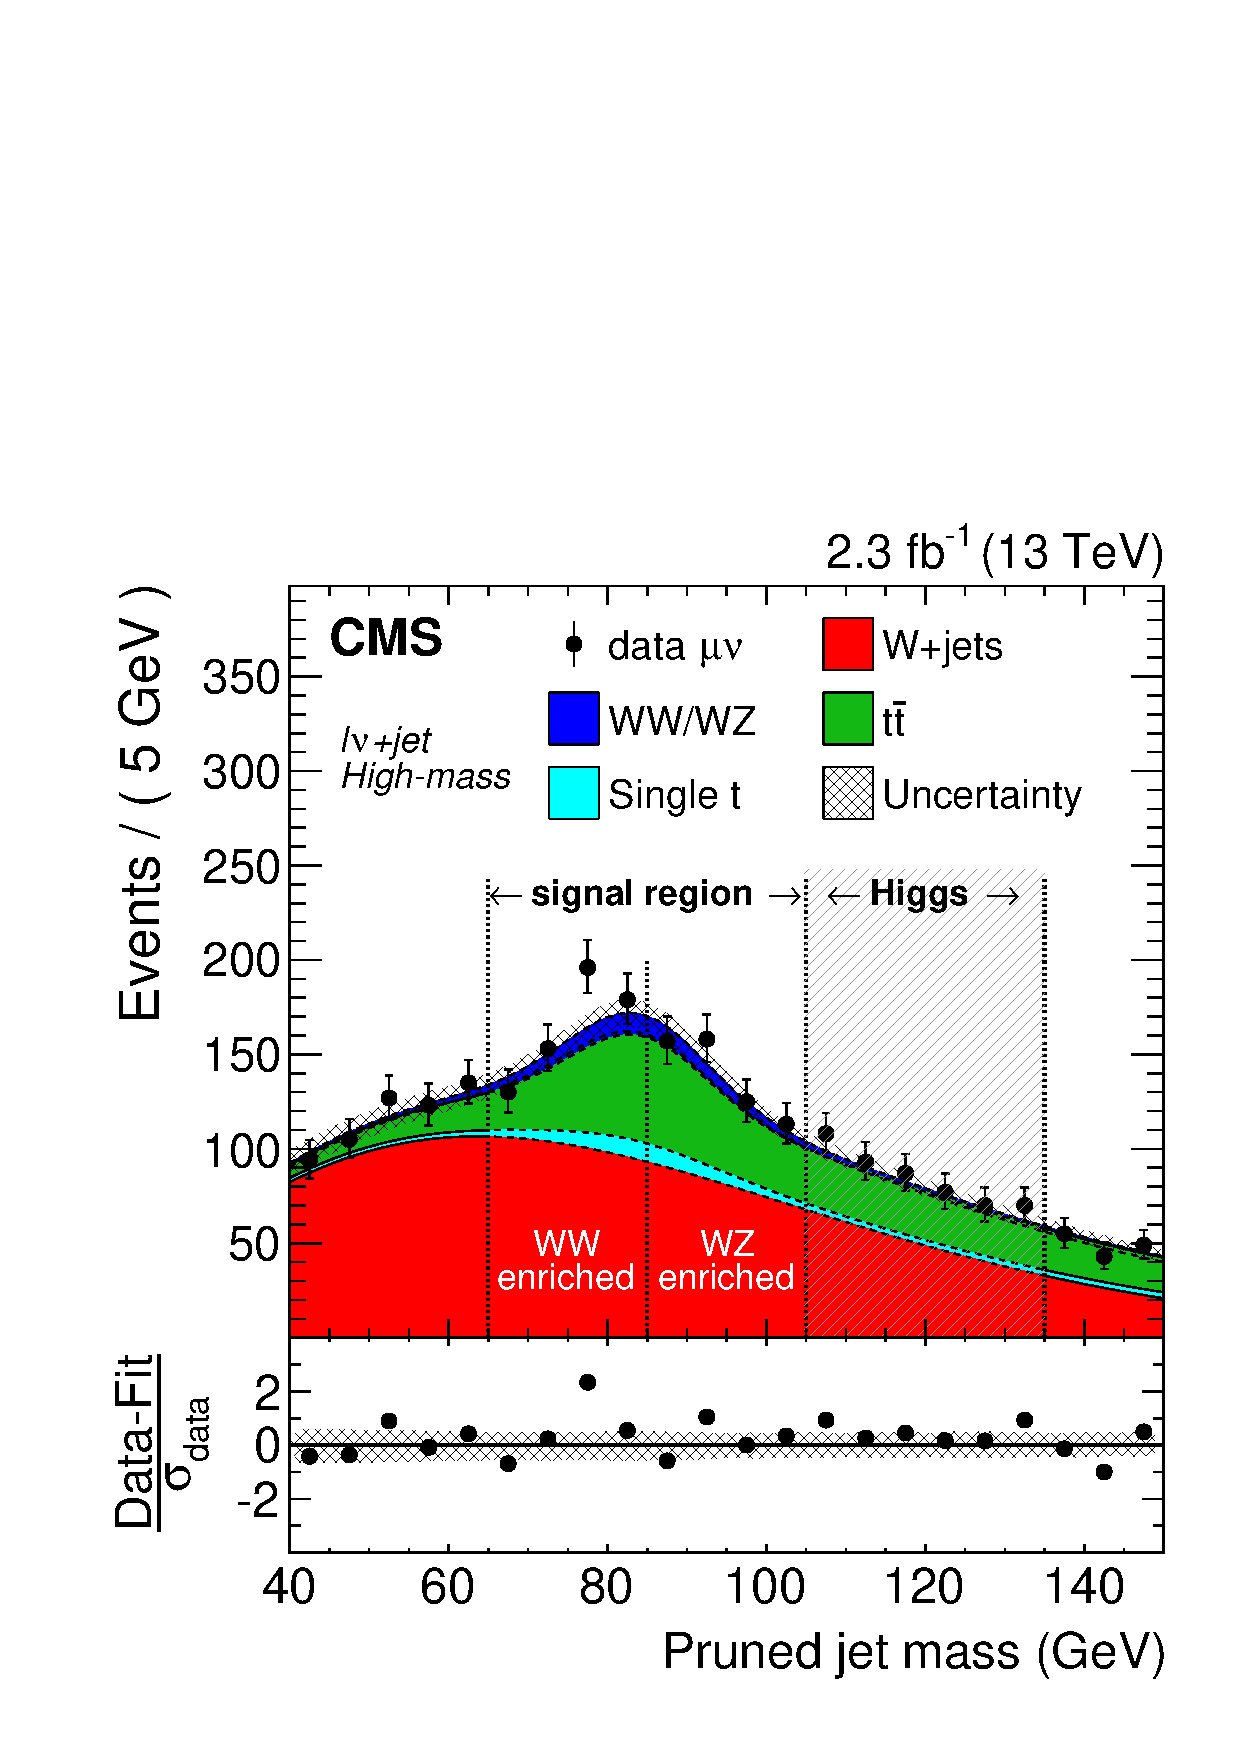
\includegraphics[width=0.45\textwidth]{\cheight/HP_mj_fitting-mu-m_j_sideband_WJets0_xww__with_pull.pdf}}
\subfigure[]{\label{fig:mjfit13TeV_b}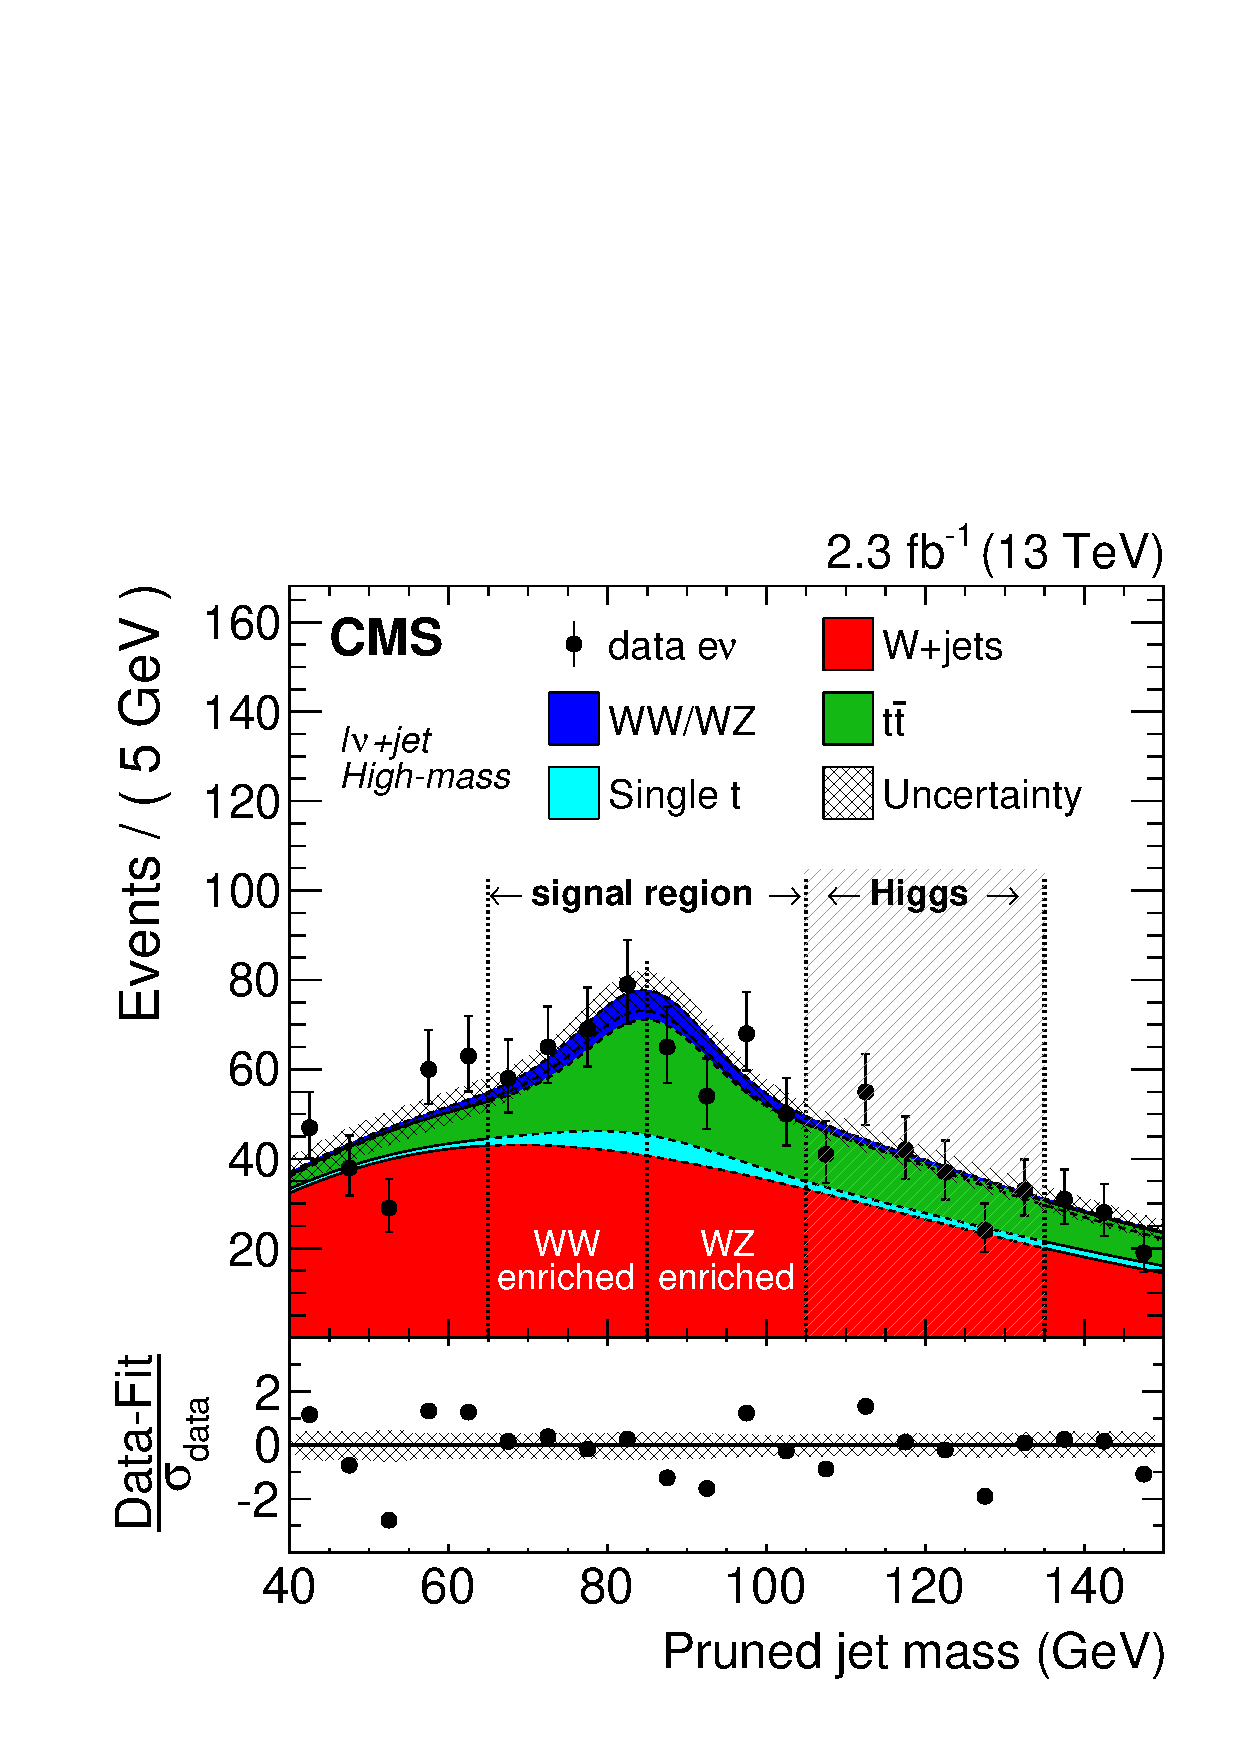
\includegraphics[width=0.45\textwidth]{\cheight/HP_mj_fitting-el-m_j_sideband_WJets0_xww__with_pull.pdf}}
\caption{Distributions in pruned jet mass in the muon (a) and electron (b) channels for the $\ell\Pgn\qqbar$ analysis at 13\TeV. All selections are applied except the requirement on the \mJ signal window. The signal regions and \mJ categories of the analysis are indicated by the vertical dotted lines. The shaded \mJ region 105--135\GeV is not used in the analysis. At the bottom of each plot, the bin-by-bin fit residuals, ($N_{\rm data}$ - $N_{\rm fit}$)/$\sigma_{\rm data}$, are shown together with the uncertainty band of the fit normalized by the statistical uncertainty of data, $\sigma_{\rm data}$.}
\label{fig:mjfit13TeV}
\end{figure}

%%%%%%%%%%%
\subsection{Extraction of the W+jets shape}~\label{subsec:wjetshape}
%%%%%%%%%%%

The form of the $\mlvj$ distribution for the W+jets background in the signal region (SR) is determined from the lower \mJ sideband, through the transfer function $\alpha_\mathrm{MC}(\mlvj)$ obtained from the W+jets simulation, and defined as:

\begin{equation}
\alpha_\mathrm{MC}(\mlvj) = \frac{F_\mathrm{MC, SR}^{\mathrm{W+jets}}(\mlvj)}{F_\mathrm{MC, SB}^{\mathrm{W+jets}}(\mlvj)},
\end{equation}

where $F_\mathrm{MC, SB}^{\mathrm{W+jets}}$ and $F_\mathrm{MC, SR}^{\mathrm{W+jets}}$ are the probability density functions used to describe the simulated \mlvj spectrum in the lower \mJ sideband and signal region, respectively.
The upper \mJ sideband is not considered since the W+jets shape is different here compared to what expected in the lower sideband. Furthermore, the upper sideband suffers from a larger \ttbar background contamination.

Since the lower sideband region does not represent a perfectly pure sample of W+jets events in data, the presence of minor backgrounds is subtracted from the observed diboson invariant mass distribution
to obtain an estimation of the W+jets contribution in the sideband control region of the data, $F_\mathrm{data, SB}^{\mathrm{W+jets}}(\mlvj)$.

The \mlvj range used in the estimate of the background distribution determines the region of masses probed by these searches.
This range is chosen to ensure a smoothly falling background spectrum, and therefore far enough from the kinematic turn-on at low masses generated by the acceptance selections,
allowing for a good stability and a robust control of the background estimation.
For this reason the low edge of the range is chosen at 0.7\TeV while the high edge is chosen such that it is not too far from the last value where data are still present.
Therefore, the fits are performed in the range $0.7 < \mlvj < 4\TeV$ for the 13\TeV analysis, while at 8\TeV no data are present above $\mlvj \approx 3\TeV$ and the chosen range is therefore $0.7 < \mlvj < 3\TeV$.

To describe the smoothly falling W+jets background distribution, a parametrization of the form of a leveled exponential is adopted, defined as

\begin{equation}\label{eqn:mVVfunct}
   F_{\rm ExpTail}(x) = e^{-\frac{x}{a+bx}}.
\end{equation}

This functional form is found to adequately describe the simulation in both the signal region and the low sideband as demonstrated in Fig.~\ref{fig:mcfits_mlvj}. Tests are performed with alternative functional forms, and the background prediction is found to agree with the one of the default function within the uncertainties.
The minor background contributions are parametrized with a simple exponential functional form, except for the diboson contribution for which the $F_{\rm ExpTail}(x)$ defined above is used.

\begin{figure}[!htb]
\centering
\subfigure[]{\label{fig:mcfits_mlvj_a}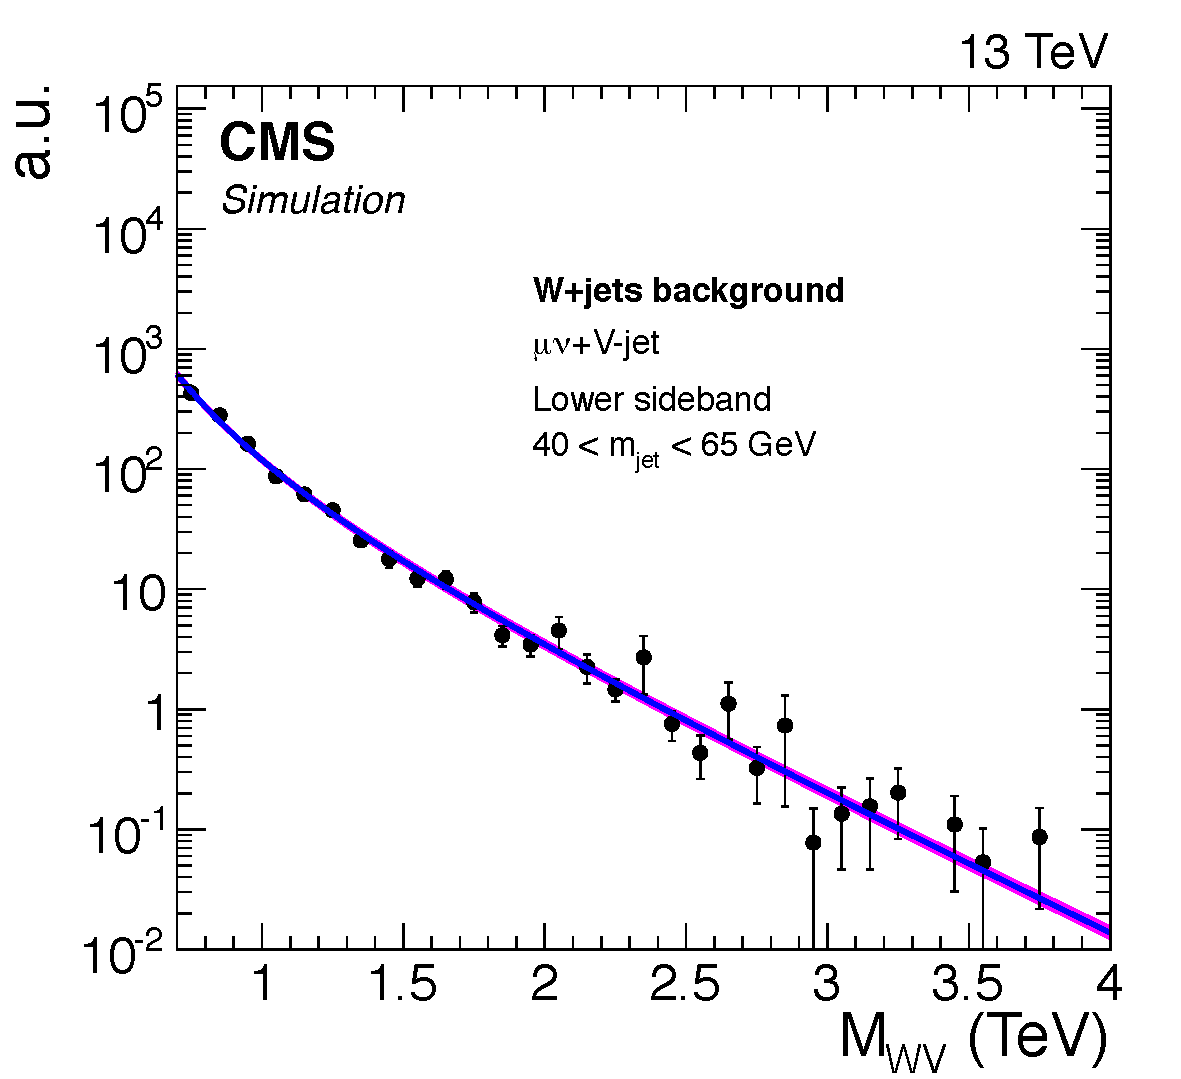
\includegraphics[width=0.32\textwidth]{\cheight/HP_mlvj_fitting_sb_lo-mu-WJets.pdf}}
\subfigure[]{\label{fig:mcfits_mlvj_b}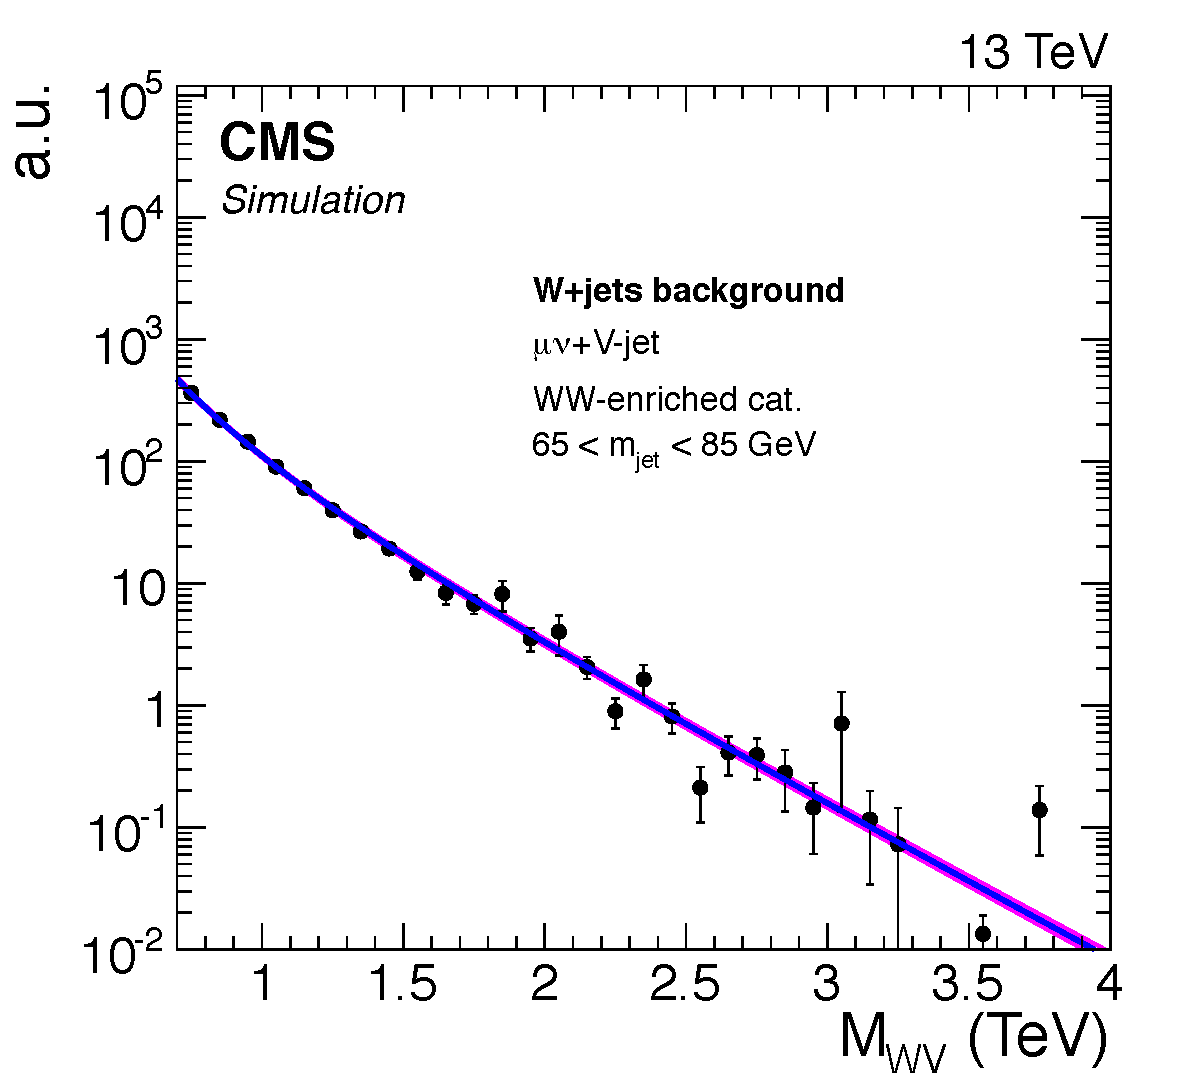
\includegraphics[width=0.32\textwidth]{\cheight/HPW_mlvj_fitting_signal_region-mu-WJets.pdf}}
\subfigure[]{\label{fig:mcfits_mlvj_c}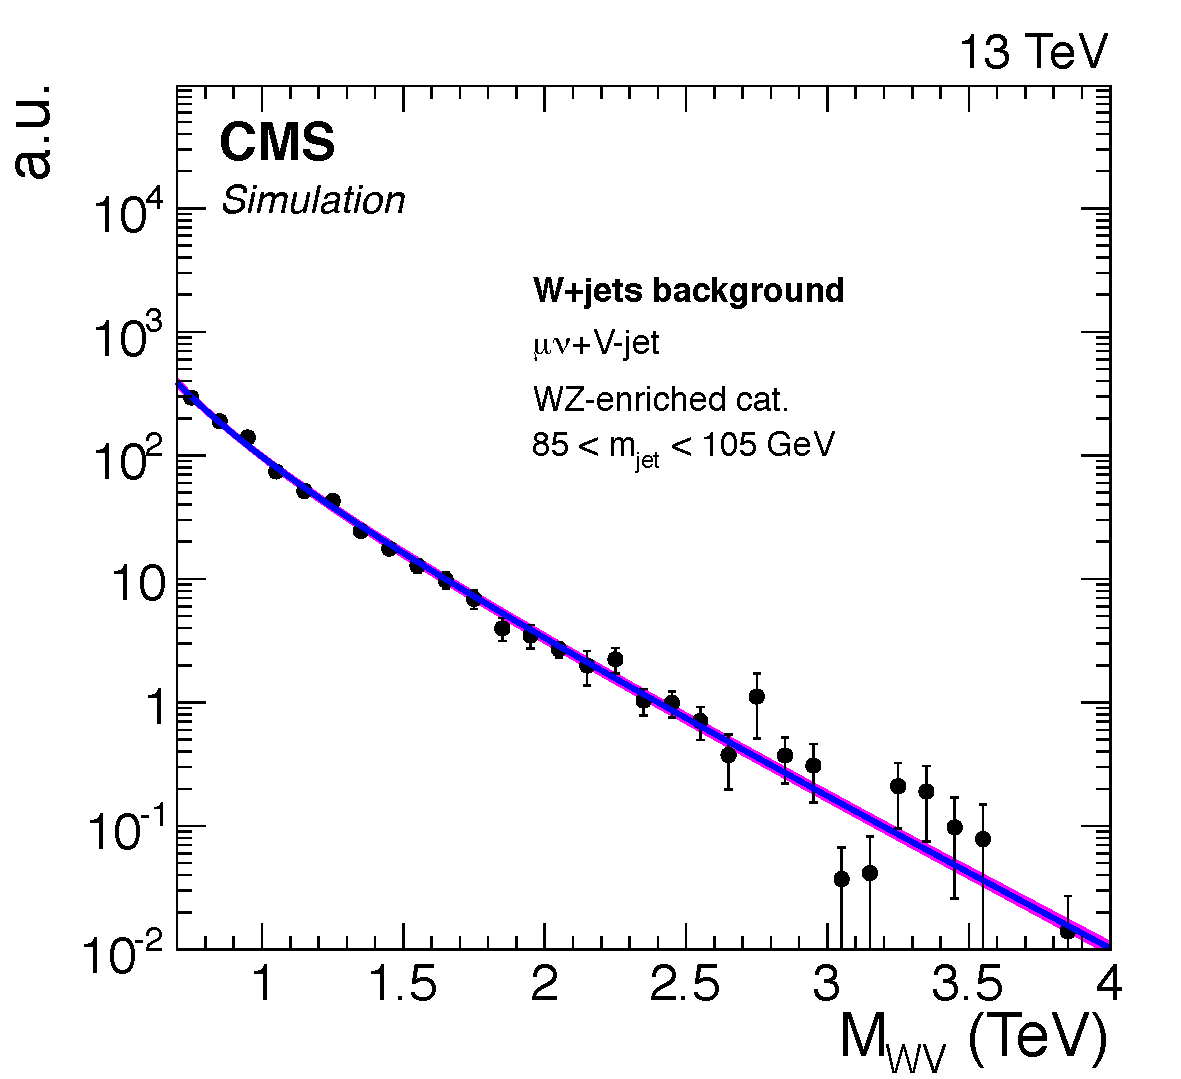
\includegraphics[width=0.32\textwidth]{\cheight/HPZ_mlvj_fitting_signal_region-mu-WJets.pdf}}
\caption{Functional form describing the diboson invariant mass spectrum of the W+jets background after fitting the simulation data. The distributions for the lower \mJ sideband (a), and the WW-enriched (b) and WZ-enriched (c) signal regions of the $\ell\nu\qqbar$ analysis are shown.}
\label{fig:mcfits_mlvj}
\end{figure}

For the $\ell\nu\qqbar$ analysis, the $\alpha_\mathrm{MC}$ is computed independently for the two WW- and WZ-enriched categories, which are therefore treated as two different signal regions.
Figure~\ref{fig:alphasWV_13TeV} shows the $\alpha_\mathrm{MC}$ for the two categories, obtained from a simultaneous fit of W+jets simulated data in the lower sideband and in the signal region defined by the category using the parametrization in Eq.~\ref{eqn:mVVfunct}.
The blue and the red lines represent the probability density functions describing the W+jets background with \mJ in the lower sideband and signal region, respectively, and given by the leveled-exponential function of Eq.~\ref{eqn:mVVfunct}. A simultaneous fit is performed of the two distributions, where the parameters used to model the distribution in the signal region are correlated with the ones used to model the distribution in the sideband.
The transfer function $\alpha_\mathrm{MC}$  is shown as a solide black line, while the dark (light) shaded region corresponds to the 1$\sigma$ (2$\sigma$) statistical uncertainty of the fit.
These uncertainties only represent the uncertainty in the modelling of the W+jets distribution. The bands have a size of approximately zero around 2\TeV as the $\alpha_\mathrm{MC}$ is the ratio of two probability density functions which have to cross in order to conserve the total probability. Similar results are obtained for the $\ell\Pgn\bbbar$ analysis.

\begin{figure}[!htb]
\centering
\subfigure[]{\label{fig:alphasWV_13TeV_a}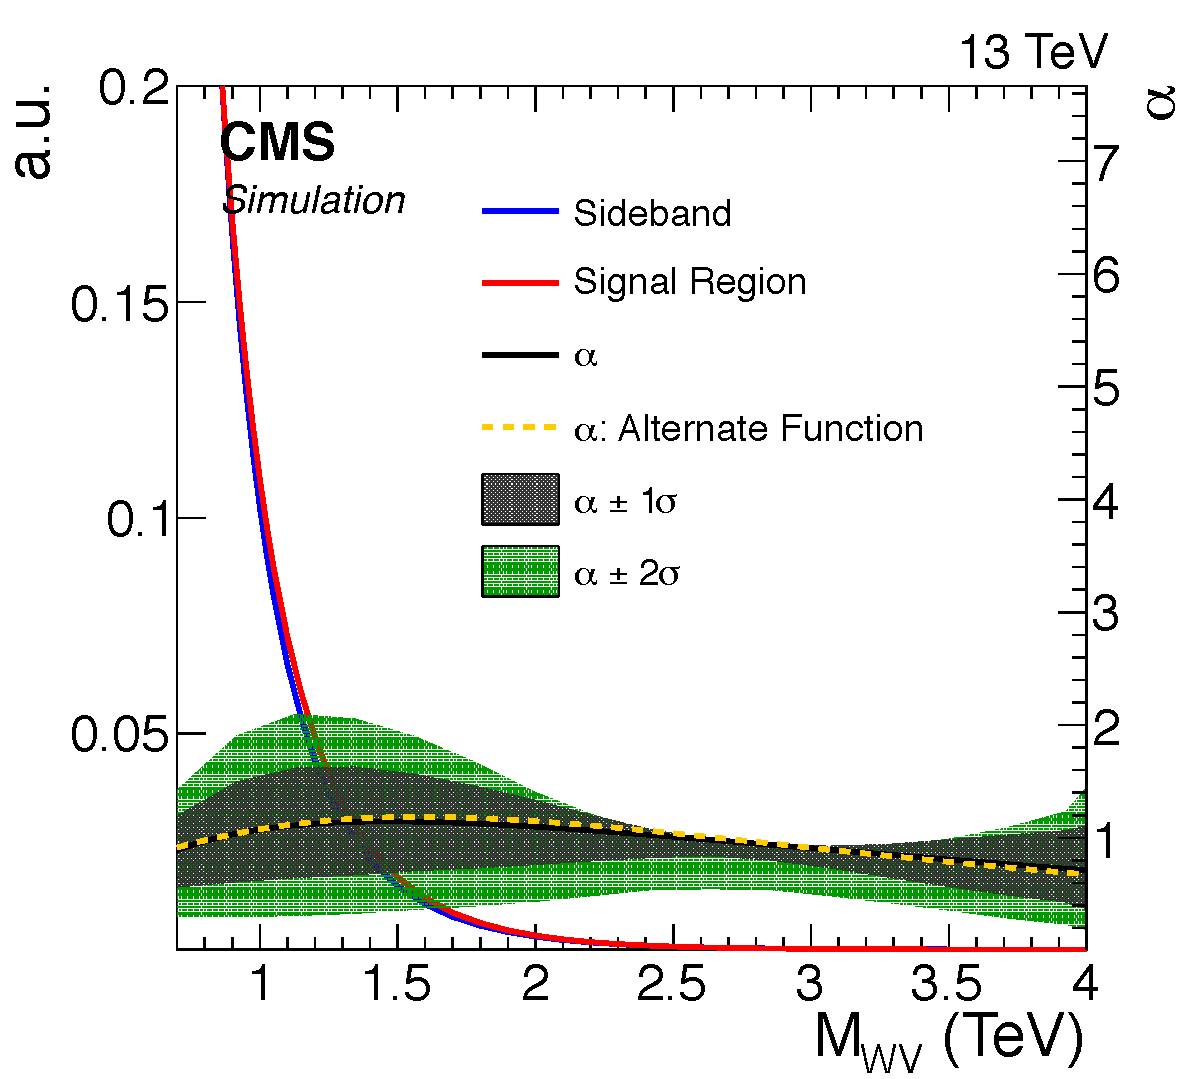
\includegraphics[width=0.45\textwidth]{\cheight/alpha_HPW-mu.pdf}}
\subfigure[]{\label{fig:alphasWV_13TeV_b}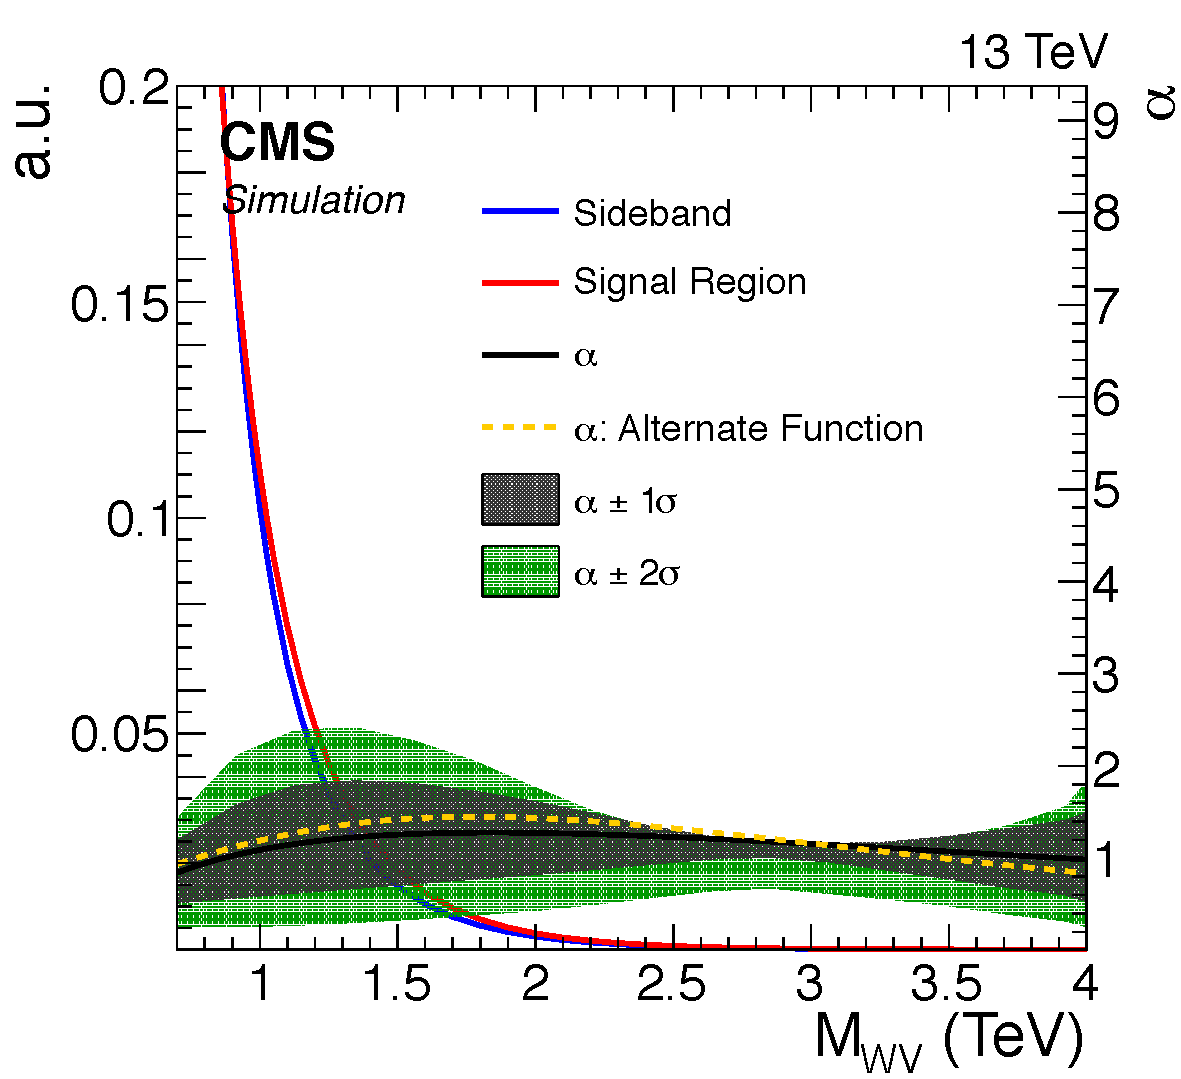
\includegraphics[width=0.45\textwidth]{\cheight/alpha_HPZ-mu.pdf}}
\caption{The transfer functions $\alpha_\mathrm{MC}$ from the lower \mJ sideband to the signal region defined by the WW-enriched (a) and WZ-enriched (b) category of the $\ell\nu\qqbar$ analysis. The dark and light shaded areas represent the statistical uncertainty of the fit. The blue and the red lines represents the probability density functions describing the W+jets background with \mJ in the lower sideband and signal region, respectively. The $\alpha_\mathrm{MC}$ obtained fitting the W+jets with and alternative function is shown as yellow line.}
\label{fig:alphasWV_13TeV}
\end{figure}

In Fig.~\ref{fig:sbfitmlvj13TeV}, the result of the fit to the \mlvj distribution of the data with \mJ in the lower sideband is shown for the electron and muon channels of the $\ell\Pgn\qqbar$ analysis.
From this fit, an estimation of $F_\mathrm{data, SB}^{\mathrm{W+jets}}(\mlvj)$ is obtained.
Finally, the W+jets background distribution in the signal region is then extrapolated by rescaling $F_\mathrm{data, SB}^{\mathrm{W+jets}}$ by $\alpha_\mathrm{MC}$.
The minor backgrounds are then added to the W+jets background to obtain the total SM prediction in the signal region, which is given by

\begin{equation}\label{eqn:alpha_totalBkg}
\footnotesize
N_\mathrm{SR}^\mathrm{bkg}(\mlvj) = N_\mathrm{SR}^\mathrm{W+jets} \times \alpha_\mathrm{MC}(\mlvj) \times F_\mathrm{data, SB}^{\mathrm{W+jets}}(\mlvj) + \sum_{k} N_\mathrm{SR}^k \times F_\mathrm{MC,SR}^k(\mlvj).
\end{equation}

In the above equation, the sum runs over the products of the normalization $N_\mathrm{MC,SR}^k$ and probability density function $F_\mathrm{MC,SR}^k$ of each minor background contribution $k$, while $N_\mathrm{SR}^\mathrm{W+jets}$ and $F_\mathrm{data, SB}^{\mathrm{W+jets}}$ represent the normalization and probability density function of the W+jets background derived from data as described previously in this chapter. The transfer function $\alpha_\mathrm{MC}$ accounts for small kinematic differences between the signal and the sideband regions.

Results of the final background extraction in the signal region will be presented in Chapters~\ref{ch:results8} and~\ref{ch:results13} or the $\ell\Pgn\bbbar$ and $\ell\Pgn\qqbar$ analysis, respectively.

\begin{figure}[!htb]
\centering
\subfigure[]{\label{fig:sbfitmlvj13TeV_a}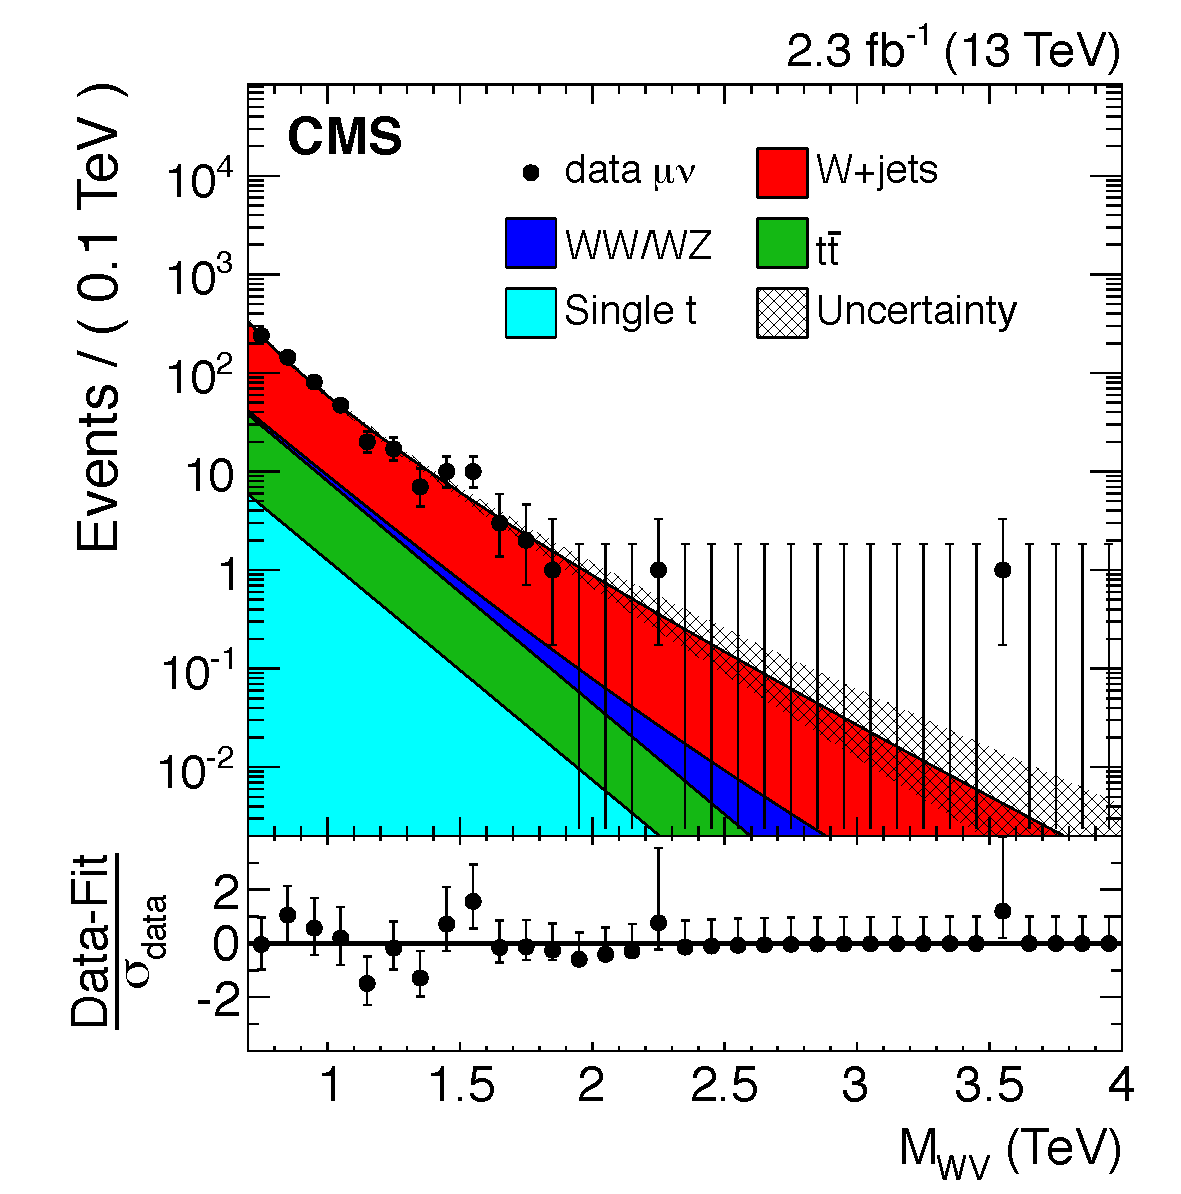
\includegraphics[width=0.45\textwidth]{\cheight/HP_m_lvj_sb_lo-mu.pdf}}
\subfigure[]{\label{fig:sbfitmlvj13TeV_b}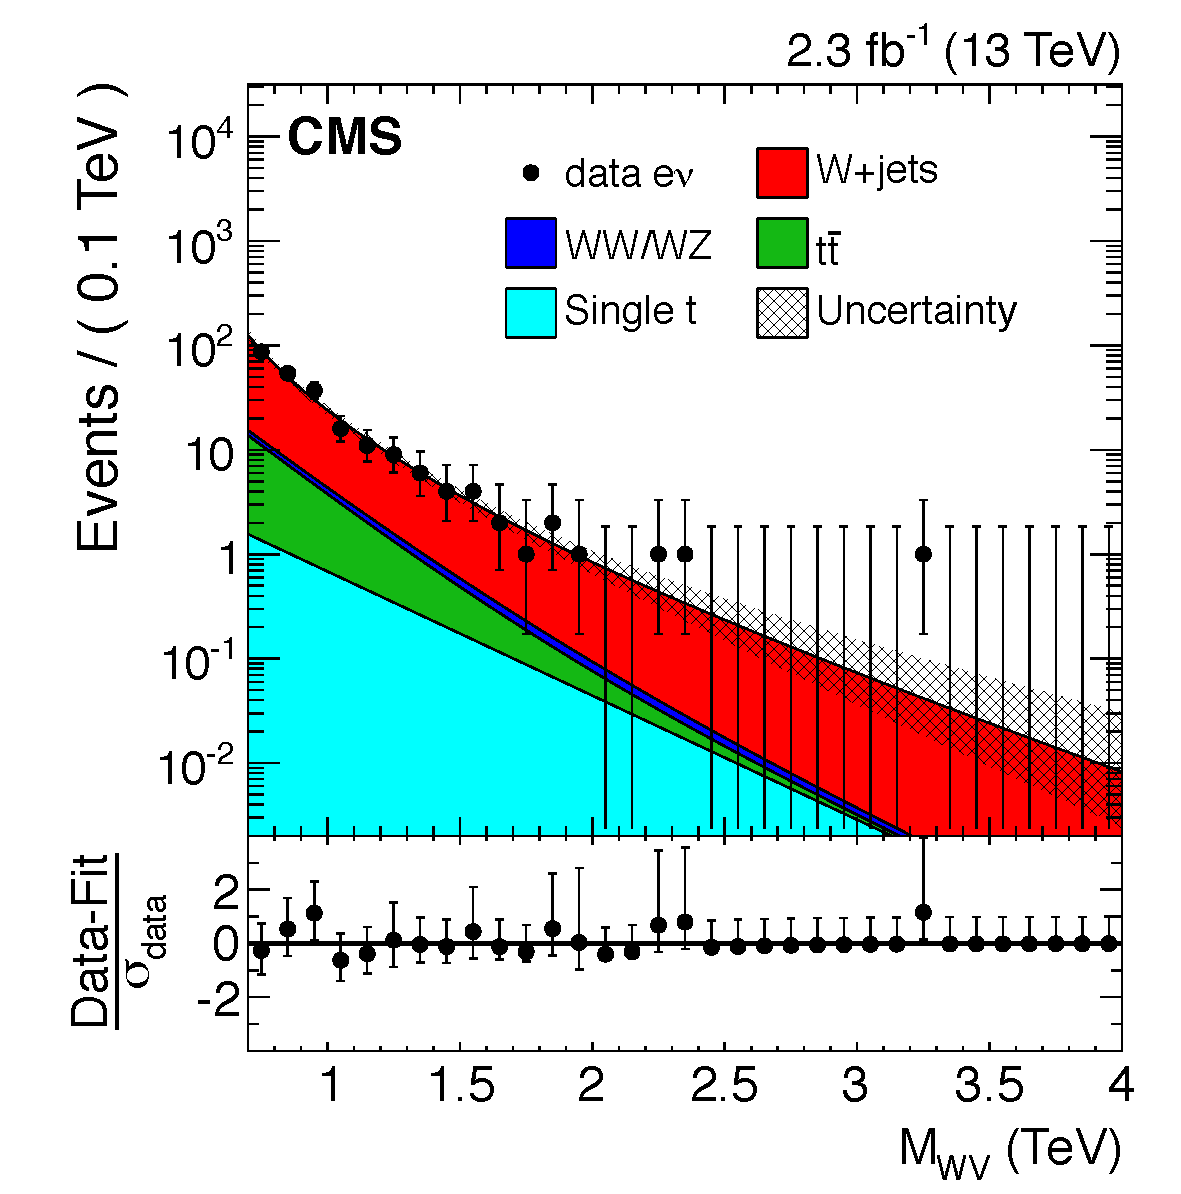
\includegraphics[width=0.45\textwidth]{\cheight/HP_m_lvj_sb_lo-el.pdf}}
\caption{Results of the fit to the \mWV distribution of the data with \mJ in the lower sideband to estimate $F_\mathrm{data, SB}^{\mathrm{W+jets}}$ for both muon (a) and electron (b) channels of the $\ell\Pgn\qqbar$ analysis. Minor backgrounds are estimated from simulation, while the W+jets contribution is the result of the fit to the data.}
\label{fig:sbfitmlvj13TeV}
\end{figure}

%%%%%%%%%%%
\subsection{Validation of the $\alpha$ method}
%%%%%%%%%%%

To test the validity and the robustness of the data driven method used to estimate the W+jets contribution and described previously in this section, a closure test is performed.
In this test, the background is extracted to a signal free control region that allows to check the compatibility with data for both the distribution and normalization.
In order to achieve this, the low mass sideband defined in Table~\ref{tab:sidebands} is divided into two regions:
$40 < \mJ < 55\GeV$, referred to as ``region A'', is used as sideband, while $55 < \mJ < 65\GeV$, referred to as ``region B'', is used as signal region.
The W+jets background normalization is then predicted in region B by performing a fit to the \mJ distribution of the data in region A and in the upper sideband (Table~\ref{tab:sidebands}),
while its distribution in \mlvj is extrapolated in region B with a fit of the data in region A and a suitable transfer function $\alpha_\mathrm{MC}$.
In this test, the $\alpha_\mathrm{MC}$ is defined as the ratio between the simulated W+jets background distributions in \mlvj in region B and A.
%The W+jets background normalization and \mlvj distribution is predicted in region B by performing a fit of the data in region A, following the procedure described previously in this section.

An example of the result of this test is presented in the following for the muon channel in the $\ell\nu\qqbar$ analysis.
%Figure~\ref{fig:mj_closureTest} shows the results of the fit to the \mJ distribution of the data inside the region A and the HSB, performed to extract the expected W+jets normalization inside the region B.
%
%\begin{figure}[!htb]
%\centering
%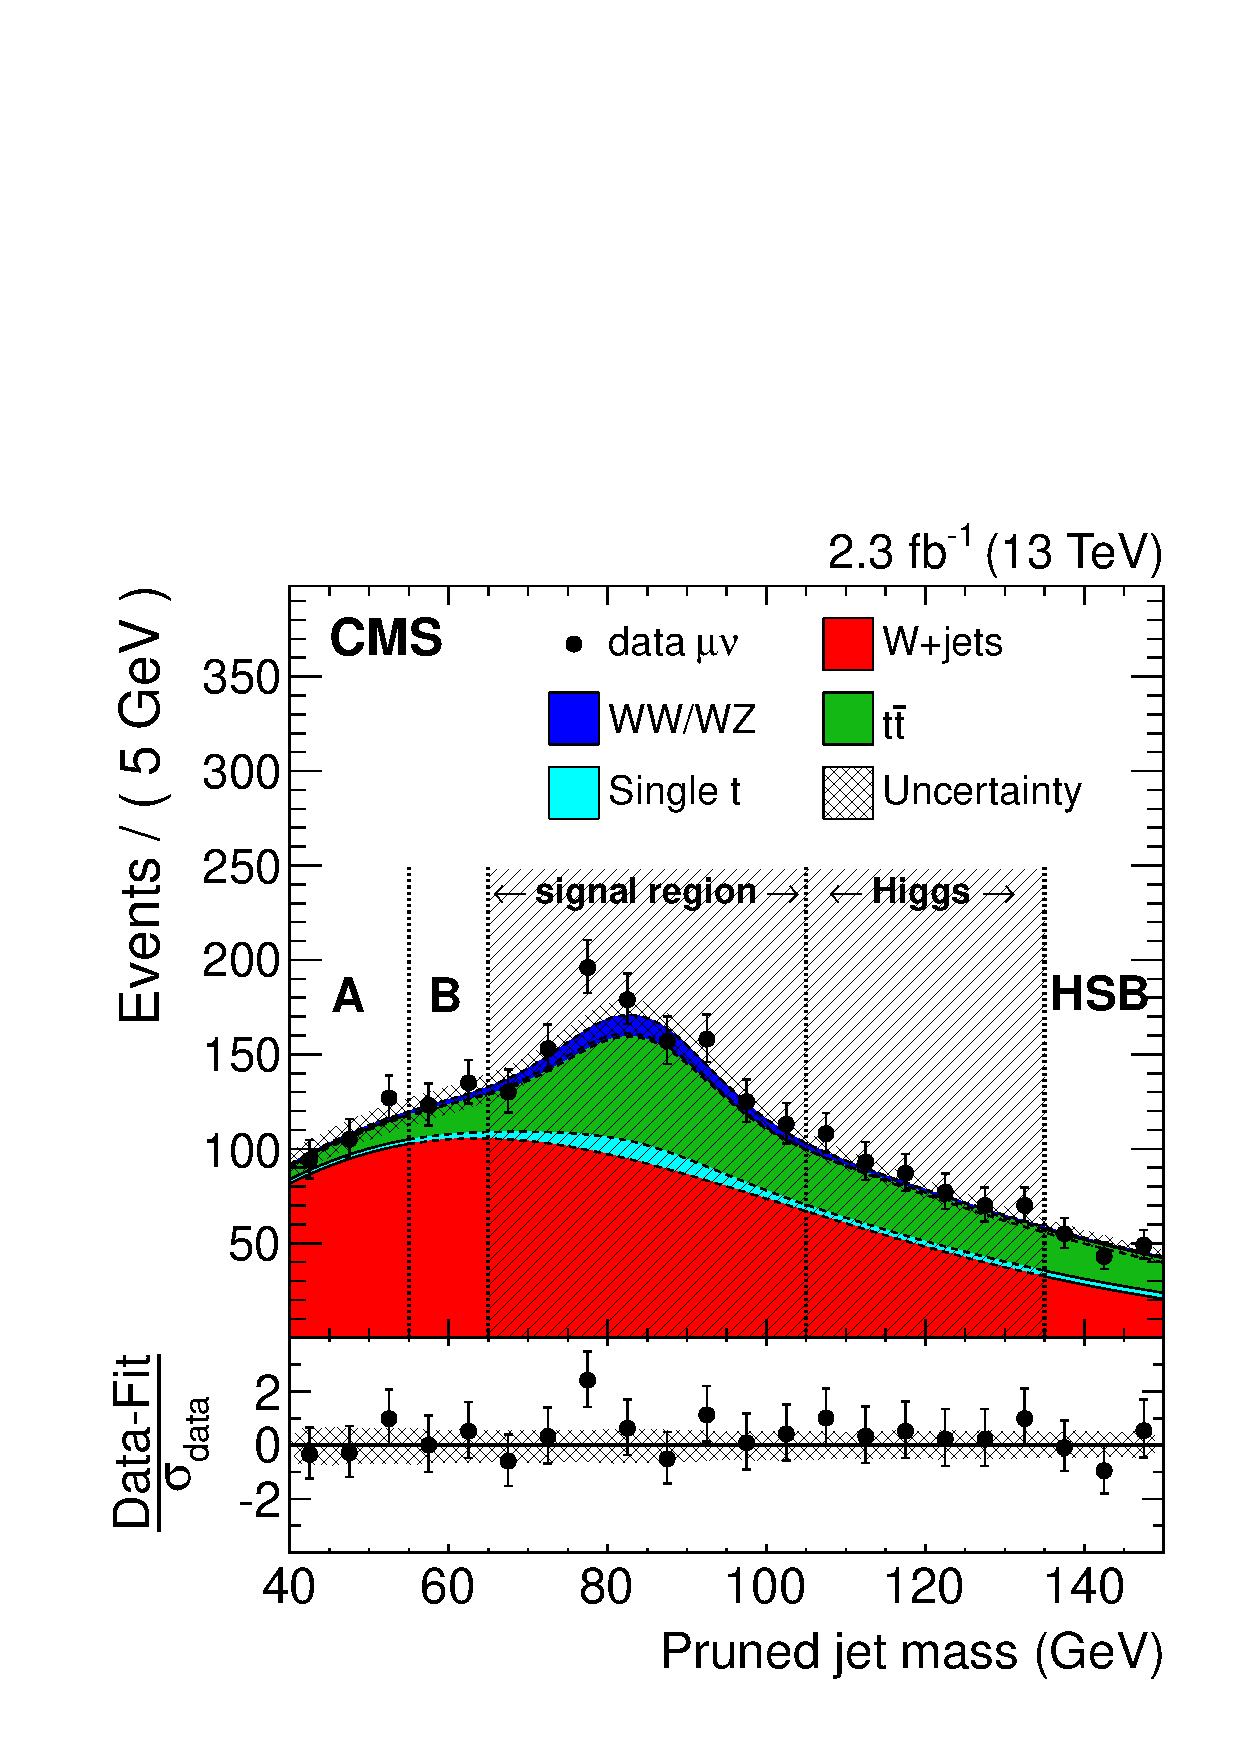
\includegraphics[width=0.5\textwidth]{\cheight/closureTest_HP_mu_mjetpruned.pdf}
%\caption{Result of the closure test for the muon channel in the $\ell\nu\qqbar$ analysis. The plot shows the fit to the pruned jet mass distribution considering only events in data with \mJ in the ranges 40--55\GeV (A) and 135--150\GeV (HSB) performed to extract the W+jets normalization inside region B.}
%\label{fig:mj_closureTest}
%\end{figure}

Figure~\ref{fig:mlvjSBandAlpha_closureTest_a} shows the transfer function $\alpha_\mathrm{MC}$ obtained from a simultaneous fit of W+jets simulated events in the region A and in the region B, using the leveled-exponential parametrization defined in Eq.~\ref{eqn:mVVfunct}. In Fig.~\ref{fig:mlvjSBandAlpha_closureTest_b}, the result of the fit to the \mlvj distribution of the data with \mJ in the lower sideband is shown, where the W+jets shape is modelled through the same leveled-exponential function.

\begin{figure}[!htb]
\centering
\subfigure[]{\label{fig:mlvjSBandAlpha_closureTest_a}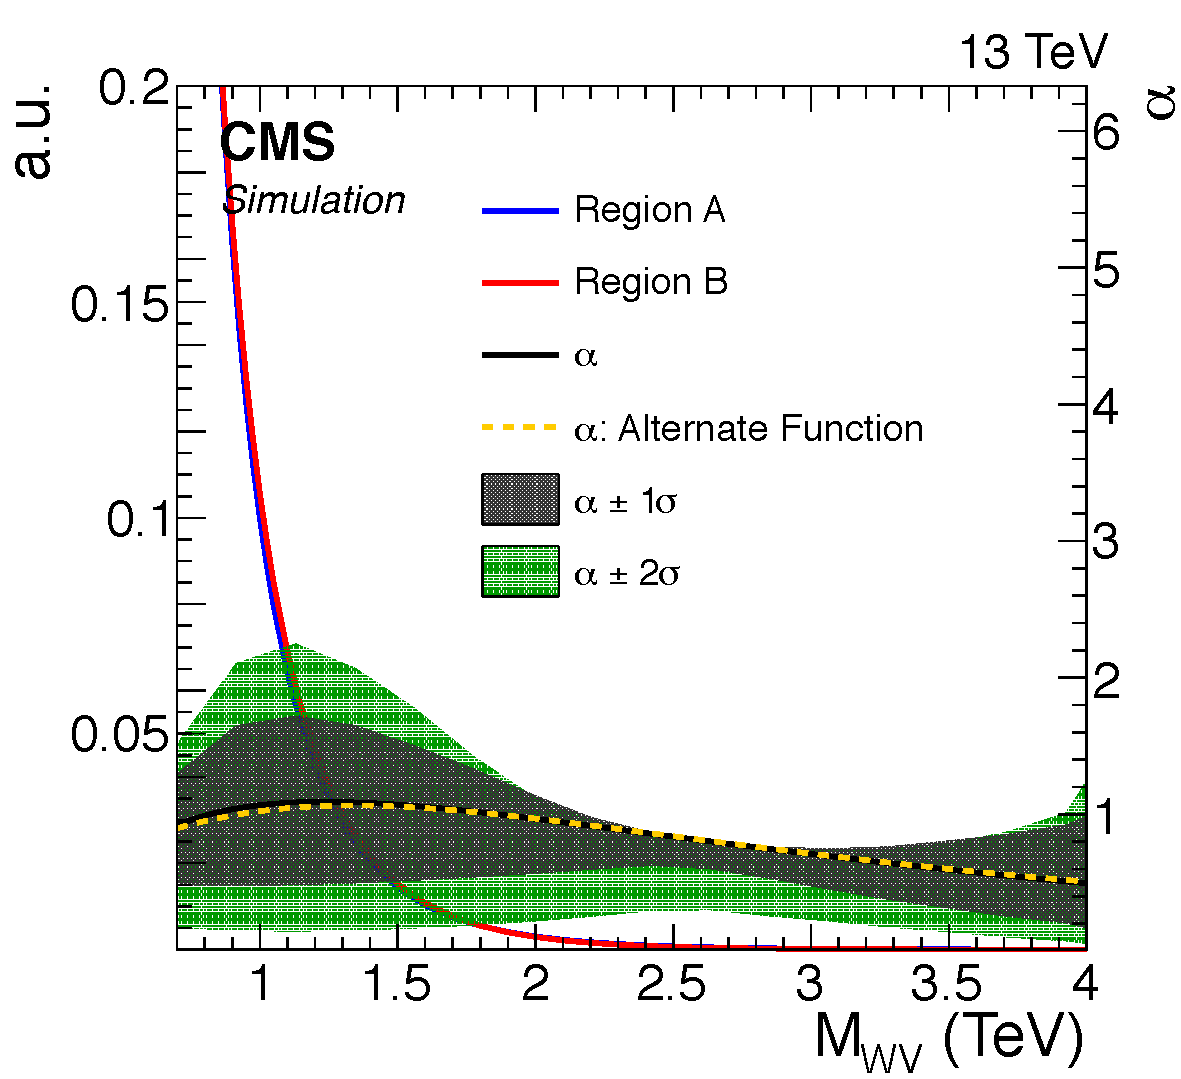
\includegraphics[width=0.47\textwidth]{\cheight/closureTest_HP_mu_alpha.pdf}}
\subfigure[]{\label{fig:mlvjSBandAlpha_closureTest_b}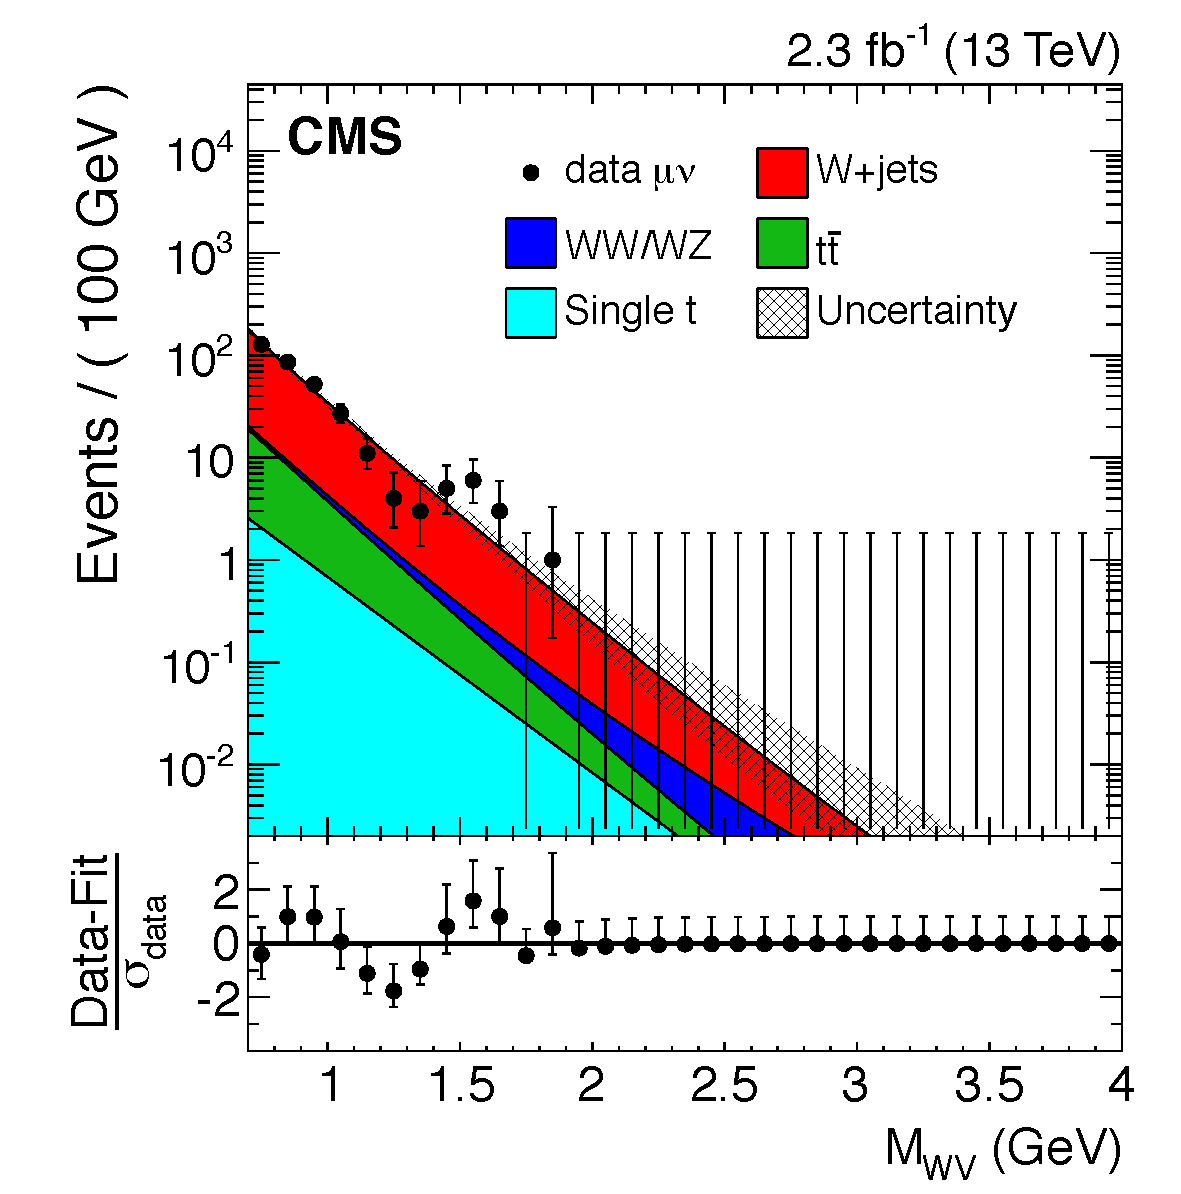
\includegraphics[width=0.43\textwidth]{\cheight/closureTest_HP_mu_regionA_mlvj.pdf}}
\caption{(a) The transfer function $\alpha_\mathrm{MC}$ obtained by simultaneously fitting the diboson invariant mass distributions of simulation data inside the sideband (A) and signal region (B). (b) Diboson invariant mass distribution for events with $40 < \mJ < 55\GeV$ (A). The W+jets shape is fitted, after subtracting contaminations from minor backgrounds, by means of a leveled-exponential function.}
\label{fig:mlvjSBandAlpha_closureTest}
\end{figure}

Finally, Fig.~\ref{fig:mlvjSR_closureTest} shows a comparison between the total predicted background, obtained through Eq.~\ref{eqn:alpha_totalBkg}, and the data inside the signal free region B.
A good agreement is found over the whole \mlvj range.
The test has been performed for both lepton flavours for the $\ell\nu\qqbar$ analysis, as well as for the $\ell\nu\bbbar$ analysis where slightly different definitions for region A and B are used.
In all the cases, consistency between the predicted background and the data is observed, thus validating the proposed strategy for the W+jets background estimation.

\begin{figure}[!htb]
\centering
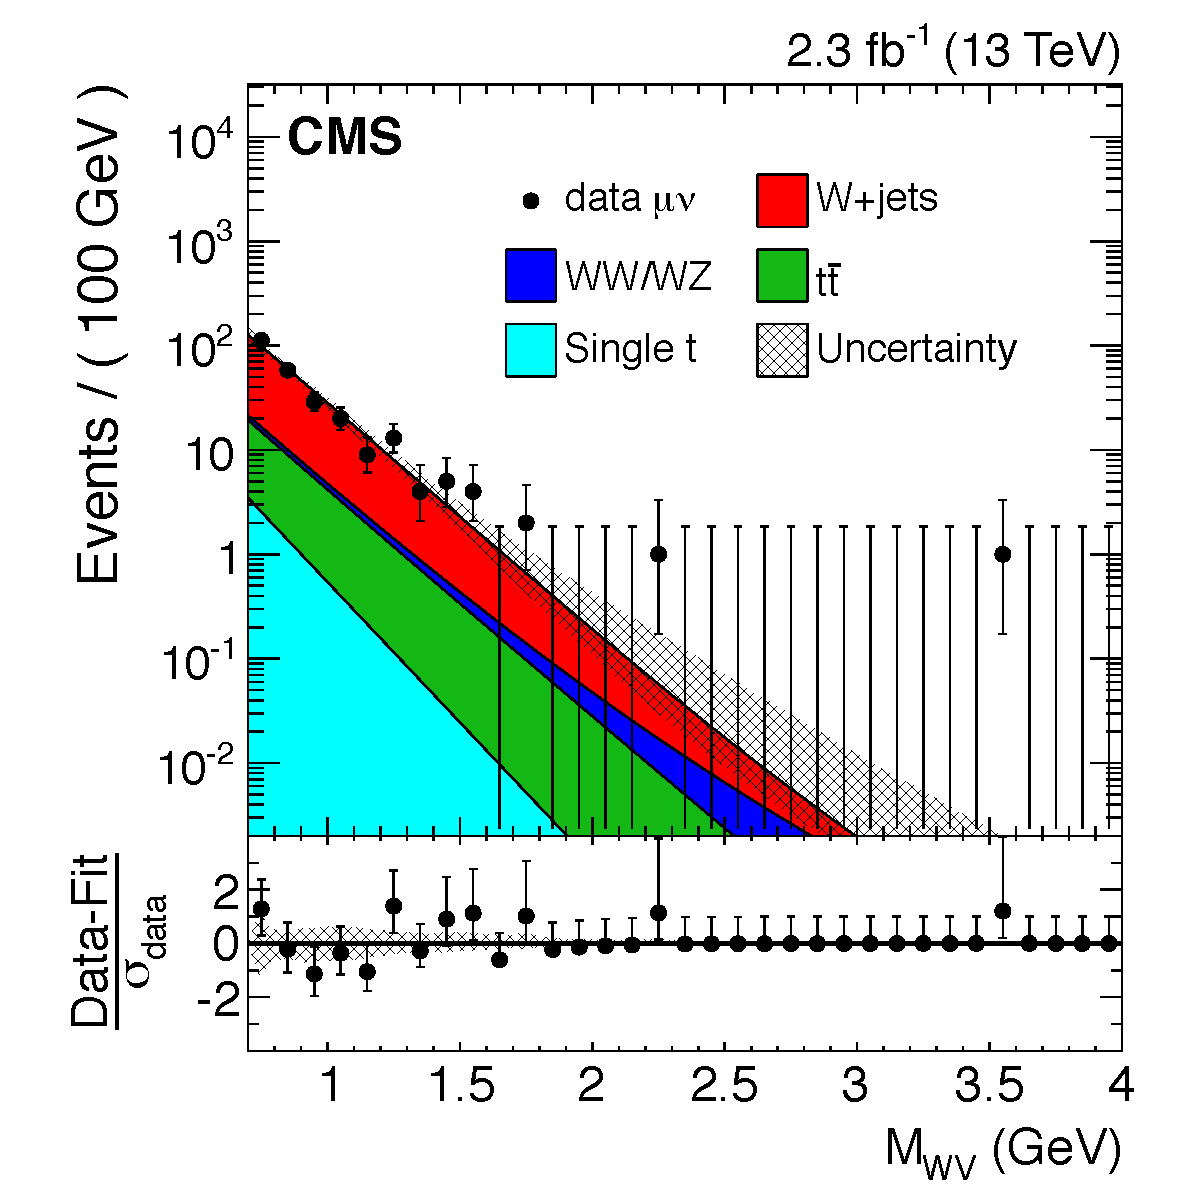
\includegraphics[width=0.5\textwidth]{\cheight/closureTest_HP_mu_regionB_mlvj.pdf}
\caption{Distributions in diboson invariant mass for data and the expected backgrounds for events inside the pruned mass region defined by $55 < \mJ < 65\GeV$ (B). The W+jets background distribution is extracted using events within $40 < \mJ < 55\GeV$ (A).}
\label{fig:mlvjSR_closureTest}
\end{figure}

%\FIXME{consider adding results with dijet function here or in the appendix}
 
 %\section{Modelling of top quark production}\label{sec:ttbar}
 %%%%%%%%%
\section{Modelling of top quark production}\label{sec:ttbar}
%%%%%%%%%

The backgrounds from \ttbar and single top quark production in both analysis channels are estimated from data-based correction factors in the normalization of the simulation.
A top quark enriched control sample is selected by applying all the analysis requirements except that the b-jet veto is inverted by requiring, instead, at least one b-tagged AK4 (or AK5) jet in the event.\\

For the $\ell\Pgn\qqbar$ channel, the comparison between data and simulation yields normalization correction factors for \ttbar and single top quark background processes evaluated in the pruned jet mass signal region
$65 < \mJ < 105\GeV$. The measured correction factors are 0.87 $\pm$ 0.04 and 0.83 $\pm$ 0.07 for the muon and electron channel, respectively, where the quoted uncertainty is only statistical.
The disagreement is consistent with the difference between NLO and NNLO shape prediction for large top quark \pt~\cite{Czakon:2015owf}.\\

For the $\ell\Pgn\bbbar$ channel, a unique correction factor is calculated with a simultaneous fit to number of data events in the muon and electron channels in the pruned jet mass region $40 < \mJ < 150\GeV$.
The difference in normalization between data and simulation is found to be 4.6 $\pm$ 5.6\%, where the quoted uncertainty is only statistical. \\

These scale factors include both the W boson signal and the combinatorial components mainly due to events where the extra b jet from the top quark decay is in the proximity of the W, and are used to correct the normalization
of the \ttbar and single top quark simulated background predictions in the signal regions. The relative uncertainties are used to quantify the uncertainty in the \ttbar and single top quark background normalization.

The \mJ distribution in the top quark enriched sample for the 13\TeV data $\ell\nu\qqbar$ analysis and for simulation is shown in Fig.~\ref{fig:tt-controlPlots13TeV_a}, while Fig.~\ref{fig:tt-controlPlots13TeV_b} shows the \nsubj distribution.
The same distribution is also shown for the $\ell\Pgn\bbbar$ analysis channel in Fig.~\ref{fig:tt-controlPlots8TeV}, where 8\TeV data and simulation are compared.
In all cases, the \mJ spectrum shows a clear peak for events with a W boson decaying to hadrons, including the combinatorial background, while a reasonable agreement between the shapes in data and simulation is observed.
Comparisons of data and simulation are also shown in Fig.~\ref{fig:tt-mtop8TeV} for other distributions such as the reconstructed \mlvj, as well as $m_\mathrm{top}^\mathrm{l}$ and $m_\mathrm{top}^\mathrm{h}$.
In the latter a clear peak at the top quark mass is visible.
%The distributions of the reconstructed $m_\mathrm{top}^\mathrm{l}$ and $m_\mathrm{top}^\mathrm{h}$ for the $\mu\Pgn$+H-jet channel are also shown in Fig.~\ref{fig:tt-mtop8TeV}, where the peak at the top quark mass is clearly visible.

\begin{figure}[!htb]
\centering
\subfigure[]{\label{fig:tt-controlPlots13TeV_a}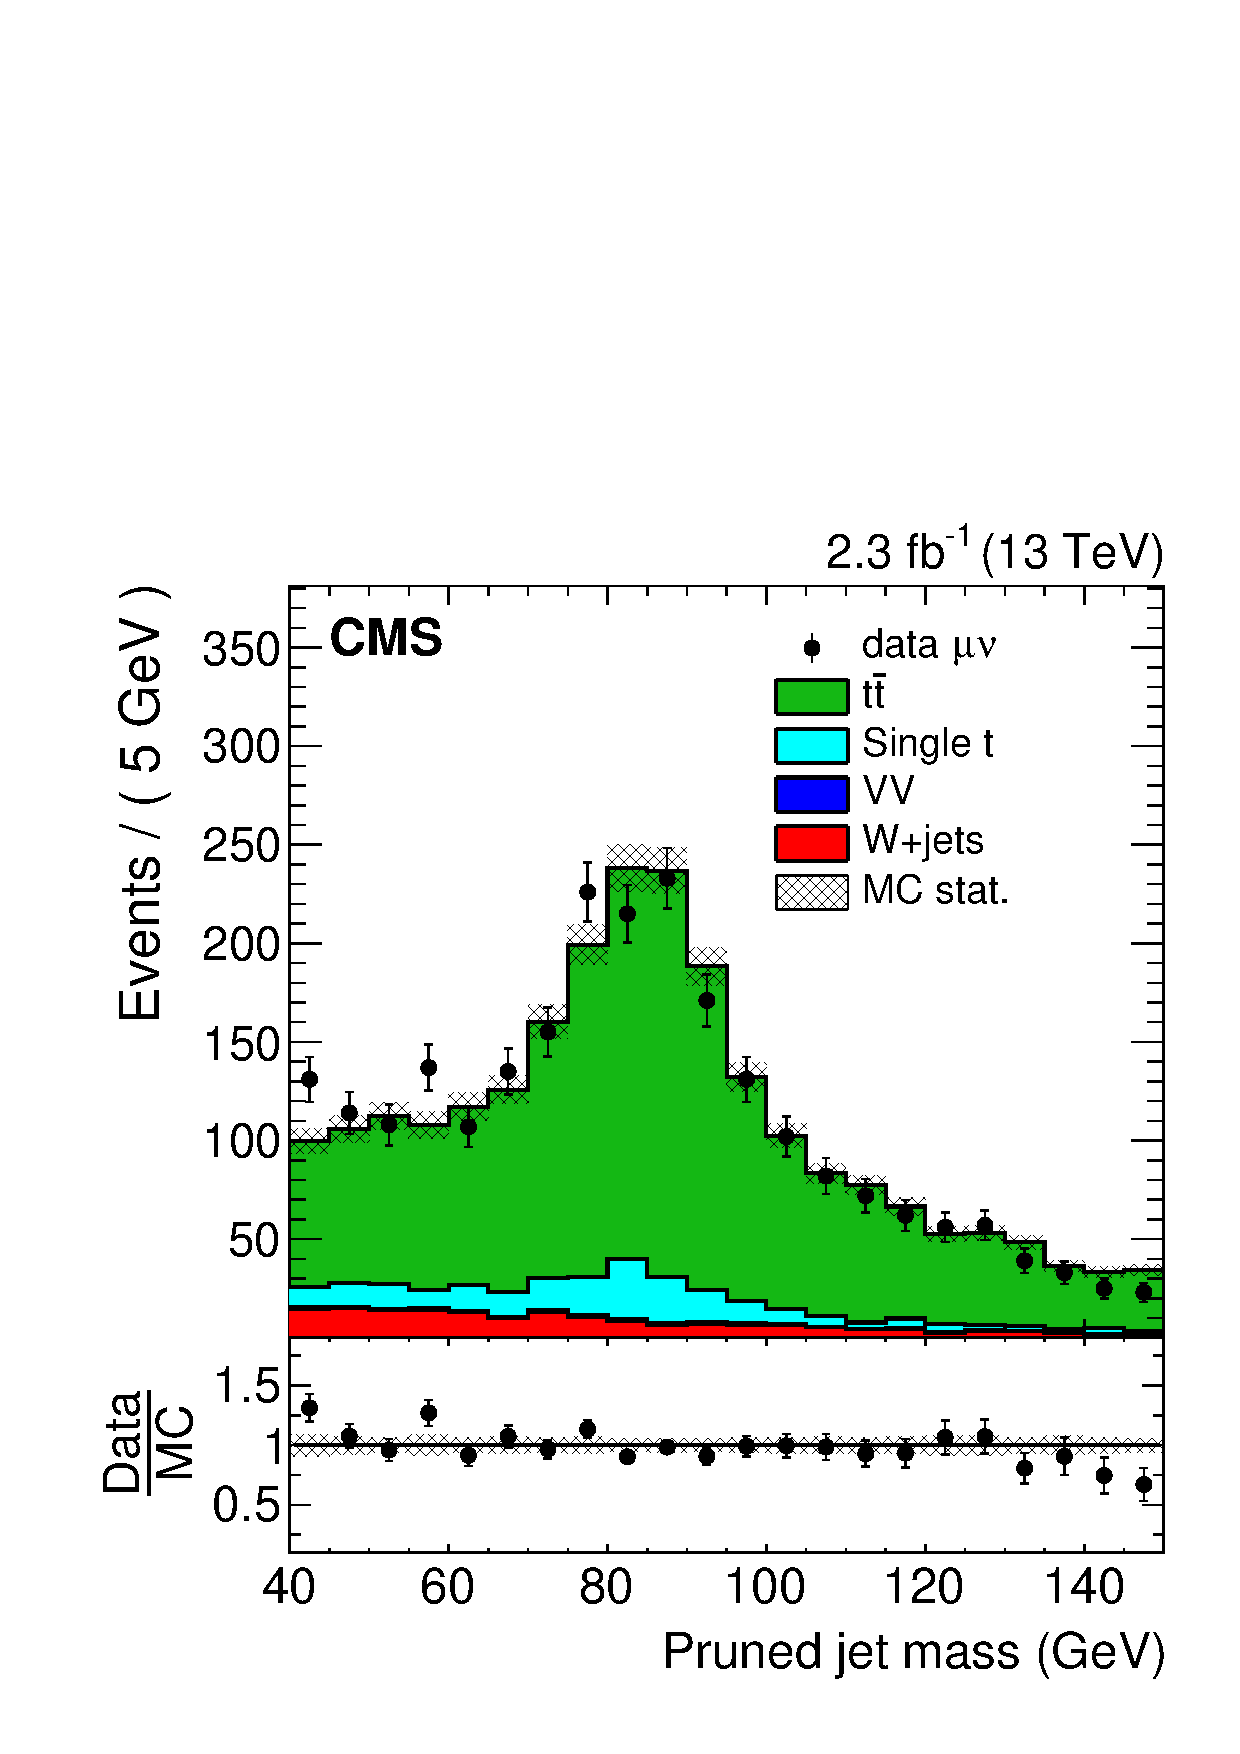
\includegraphics[width=0.45\textwidth]{\cheight/ttbar-pruned-jet-mass-mu-13TeV.pdf}}
\subfigure[]{\label{fig:tt-controlPlots13TeV_b}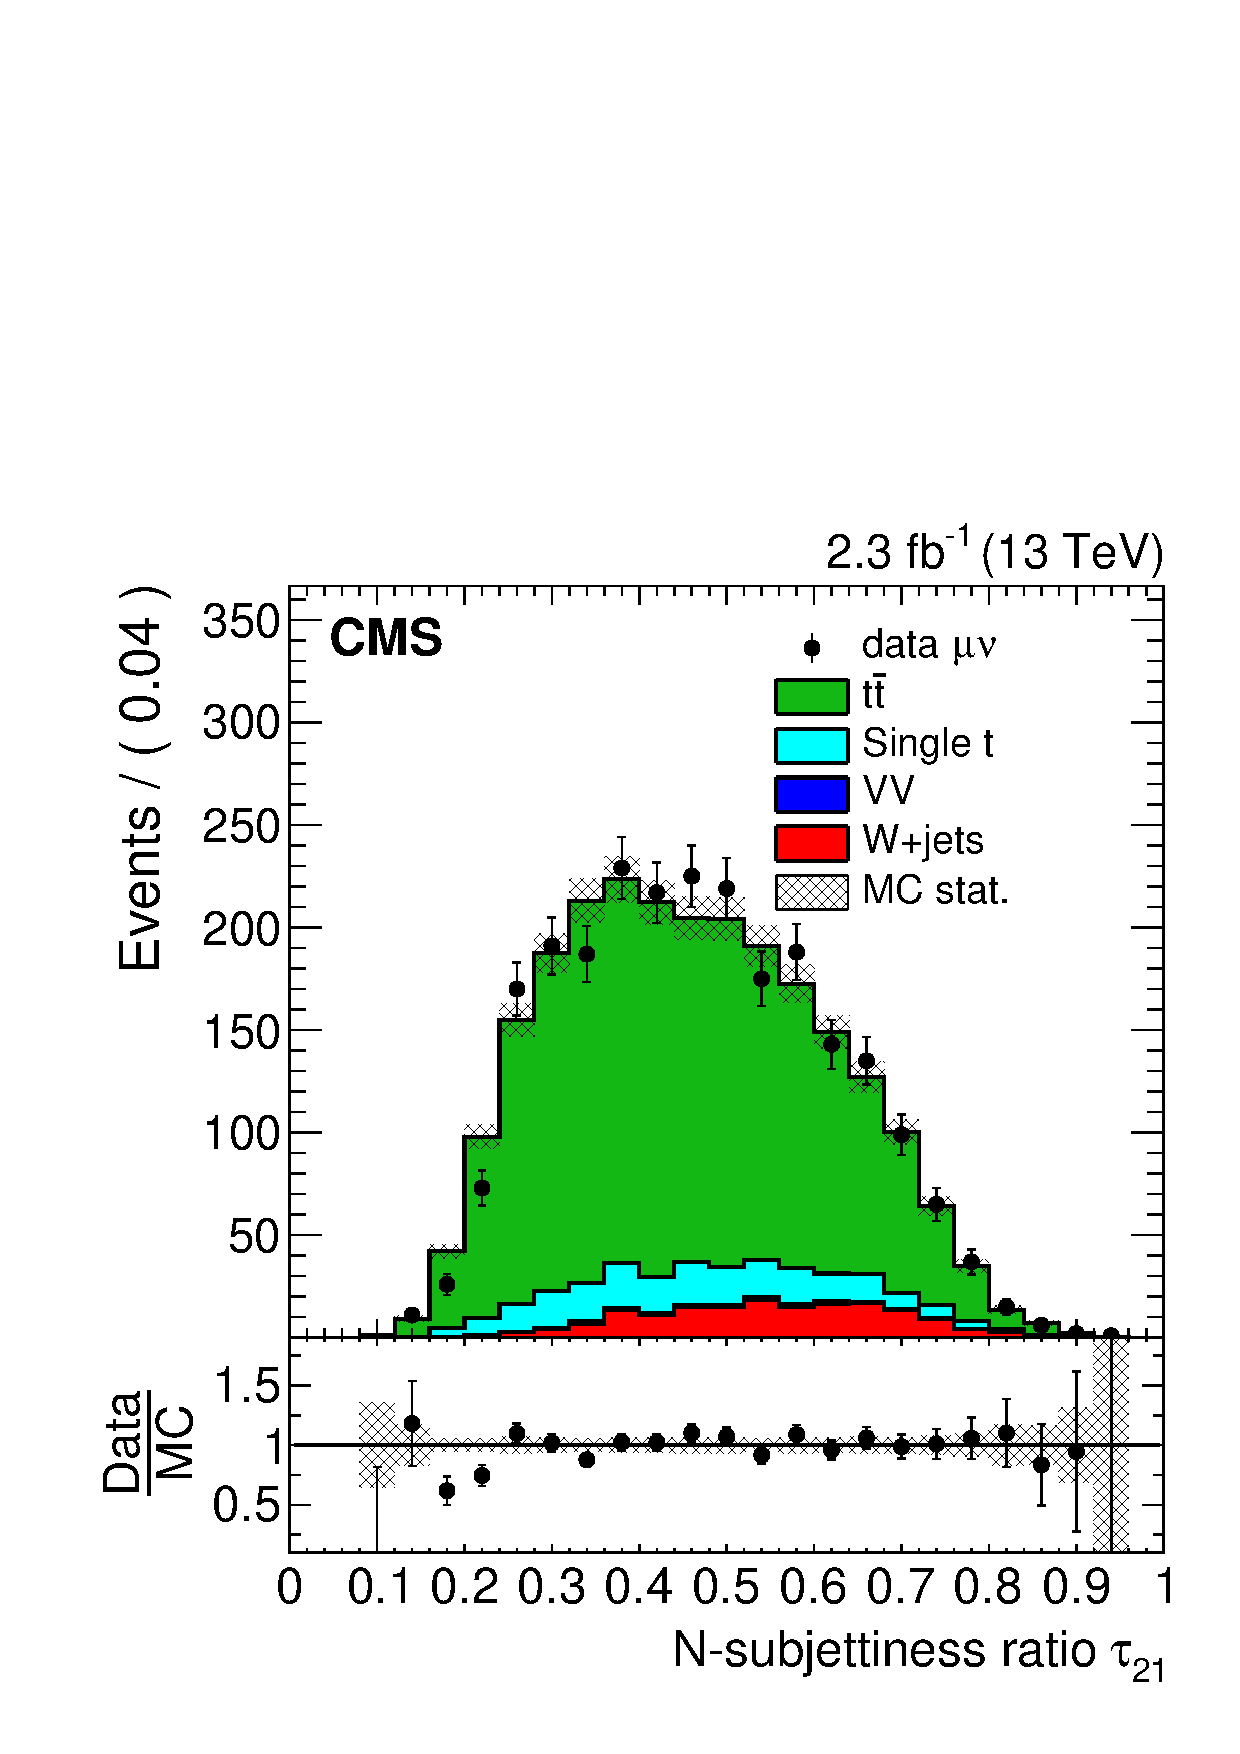
\includegraphics[width=0.45\textwidth]{\cheight/ttbar-tau21-mu-13TeV.pdf}}
\caption{Distributions in the N-subjettiness ratio \nsubj (a) and pruned jet mass \mJ (b) from the top quark enriched control sample in the muon channel of the $\ell\nu\qqbar$ analysis. The \ttbar background is rescaled such that the total number of background events matches the number of events in 13\TeV data.}
\label{fig:tt-controlPlots13TeV}
\end{figure}

\begin{figure}[!htb]
\centering
\subfigure[]{\label{fig:tt-controlPlots8TeV_a}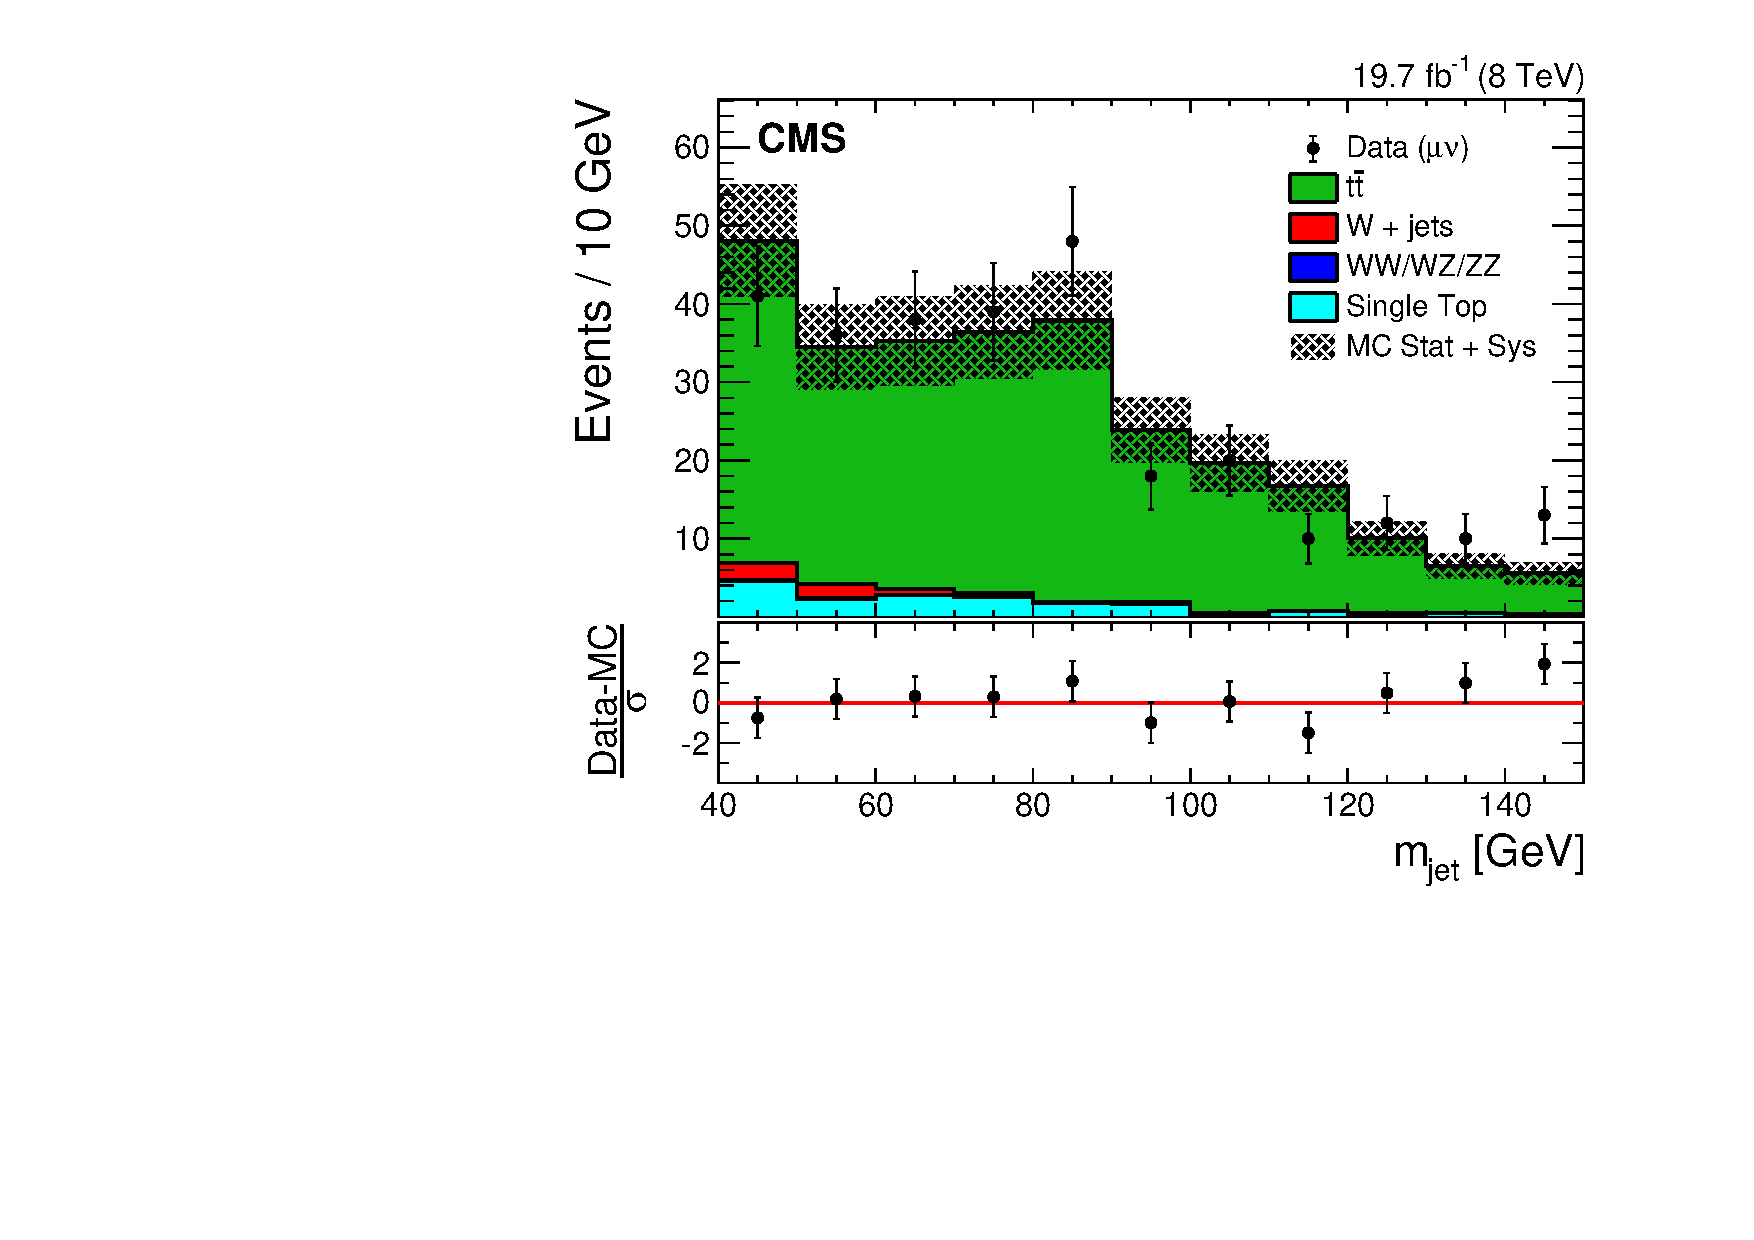
\includegraphics[width=0.45\textwidth]{\cheight/ttbar-pruned-jet-mass-mu-8TeV.pdf}}
\subfigure[]{\label{fig:tt-controlPlots8TeV_b}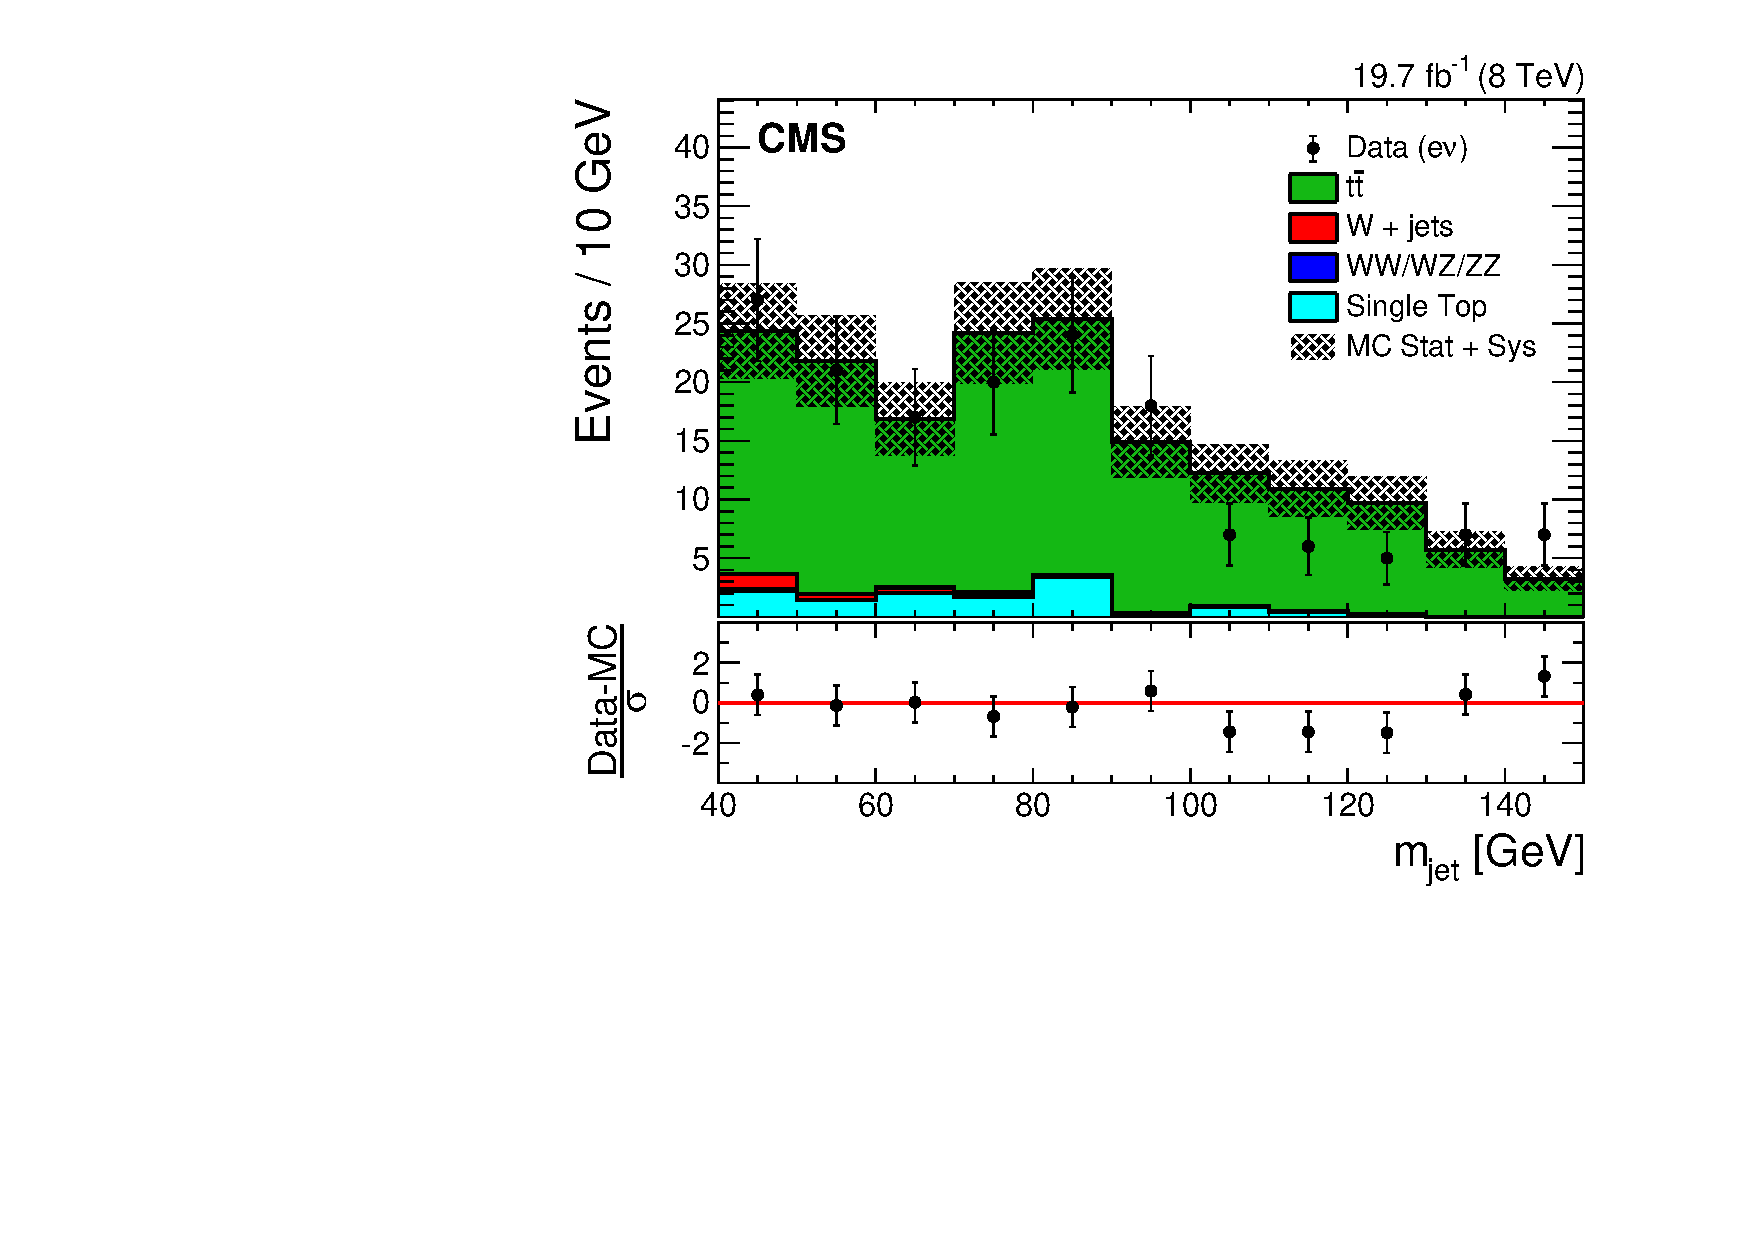
\includegraphics[width=0.45\textwidth]{\cheight/ttbar-pruned-jet-mass-e-8TeV.pdf}}
\caption{Distributions in pruned jet mass \mJ in the top quark enriched control sample in the electron (a) and muon (b) channels of the $\ell\Pgn\bbbar$ analysis. The hatched region indicates the overall uncertainty in the background. In the lower panels, the bin-by-bin residuals, (Data - MC)/$\sigma$ are shown, where $\sigma$ is the sum in quadrature of the statistical uncertainty of the 8\TeV data, the simulation, and the systematic uncertainty in the \ttbar background.}
\label{fig:tt-controlPlots8TeV}
\end{figure}

\begin{figure}[!htb]
\centering
\subfigure[]{\label{fig:tt-mtop8TeV_a}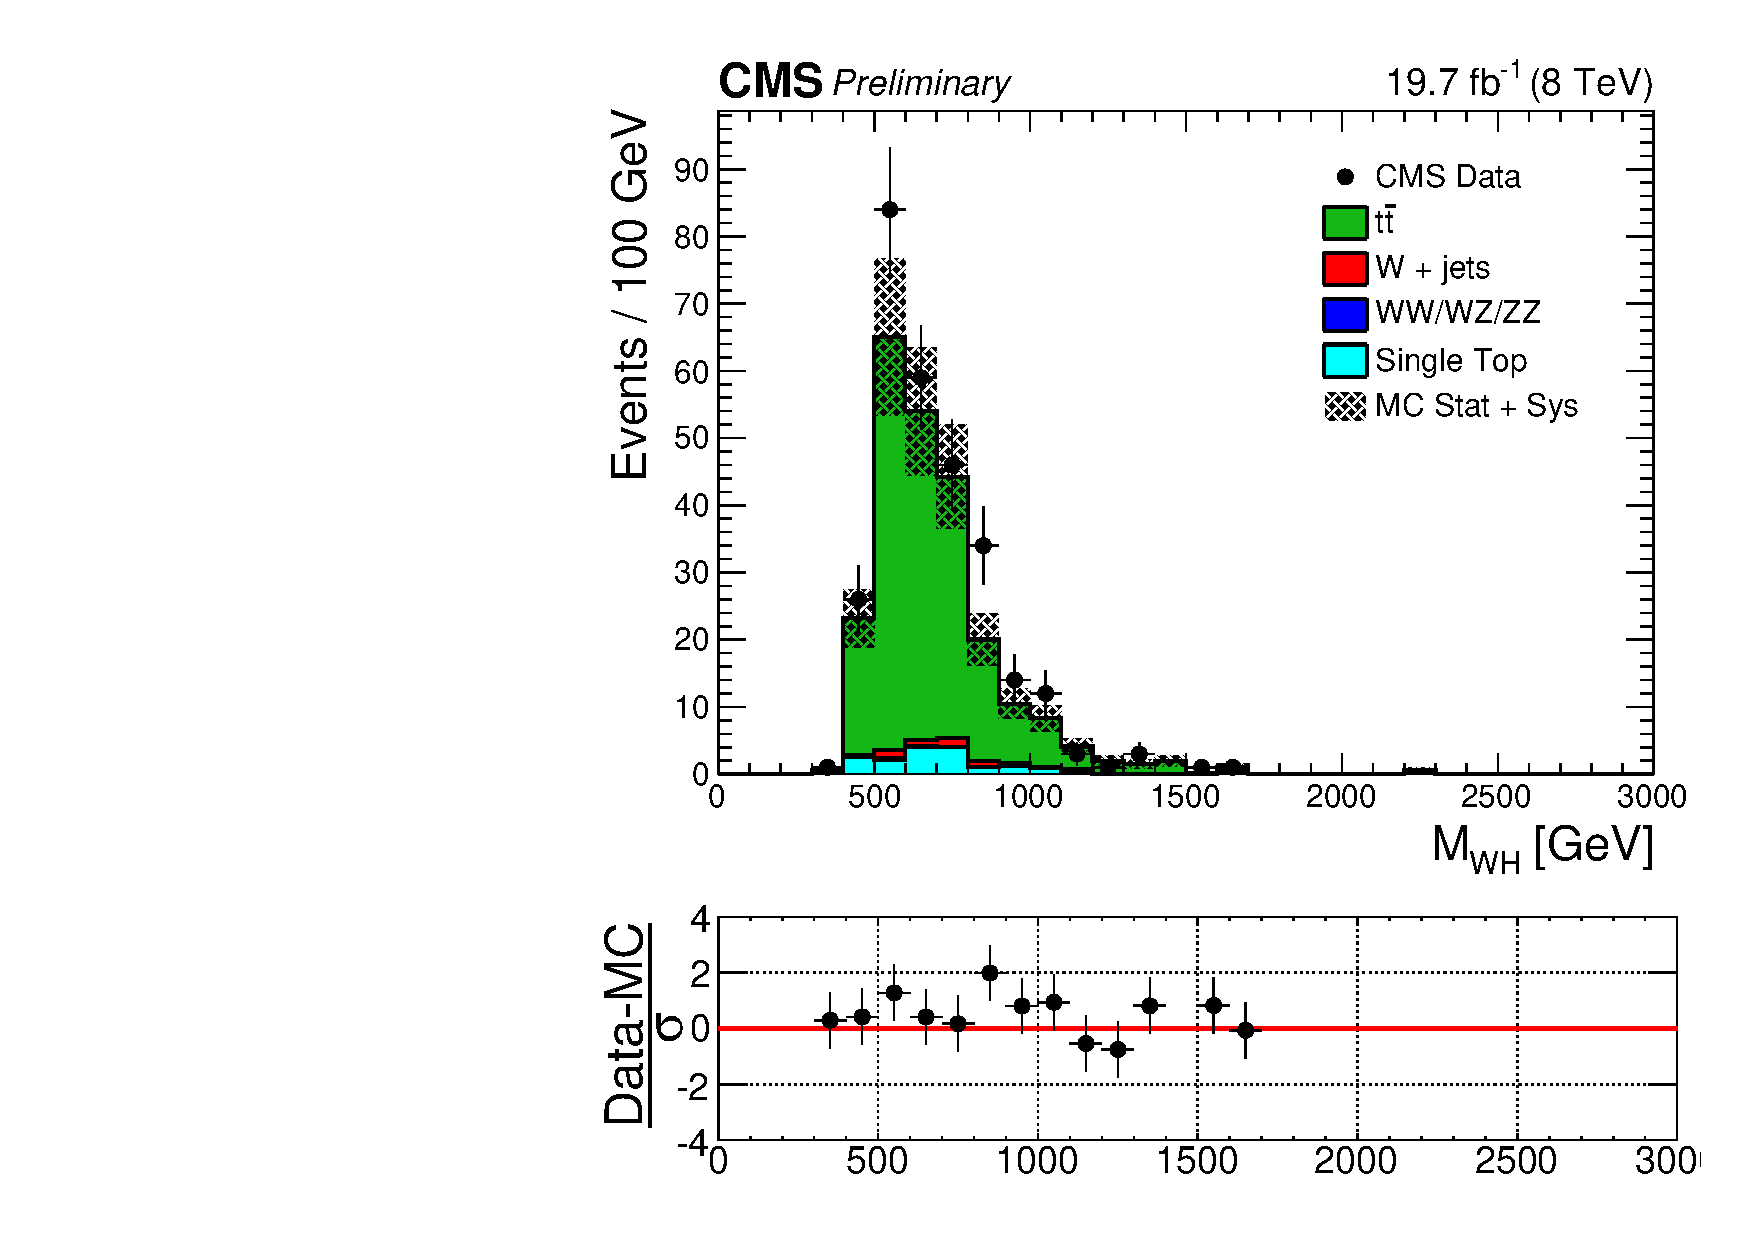
\includegraphics[width=0.45\textwidth]{\cheight/ttbar-dibosons-invmass-8TeV.pdf}}\\
\subfigure[]{\label{fig:tt-mtop8TeV_b}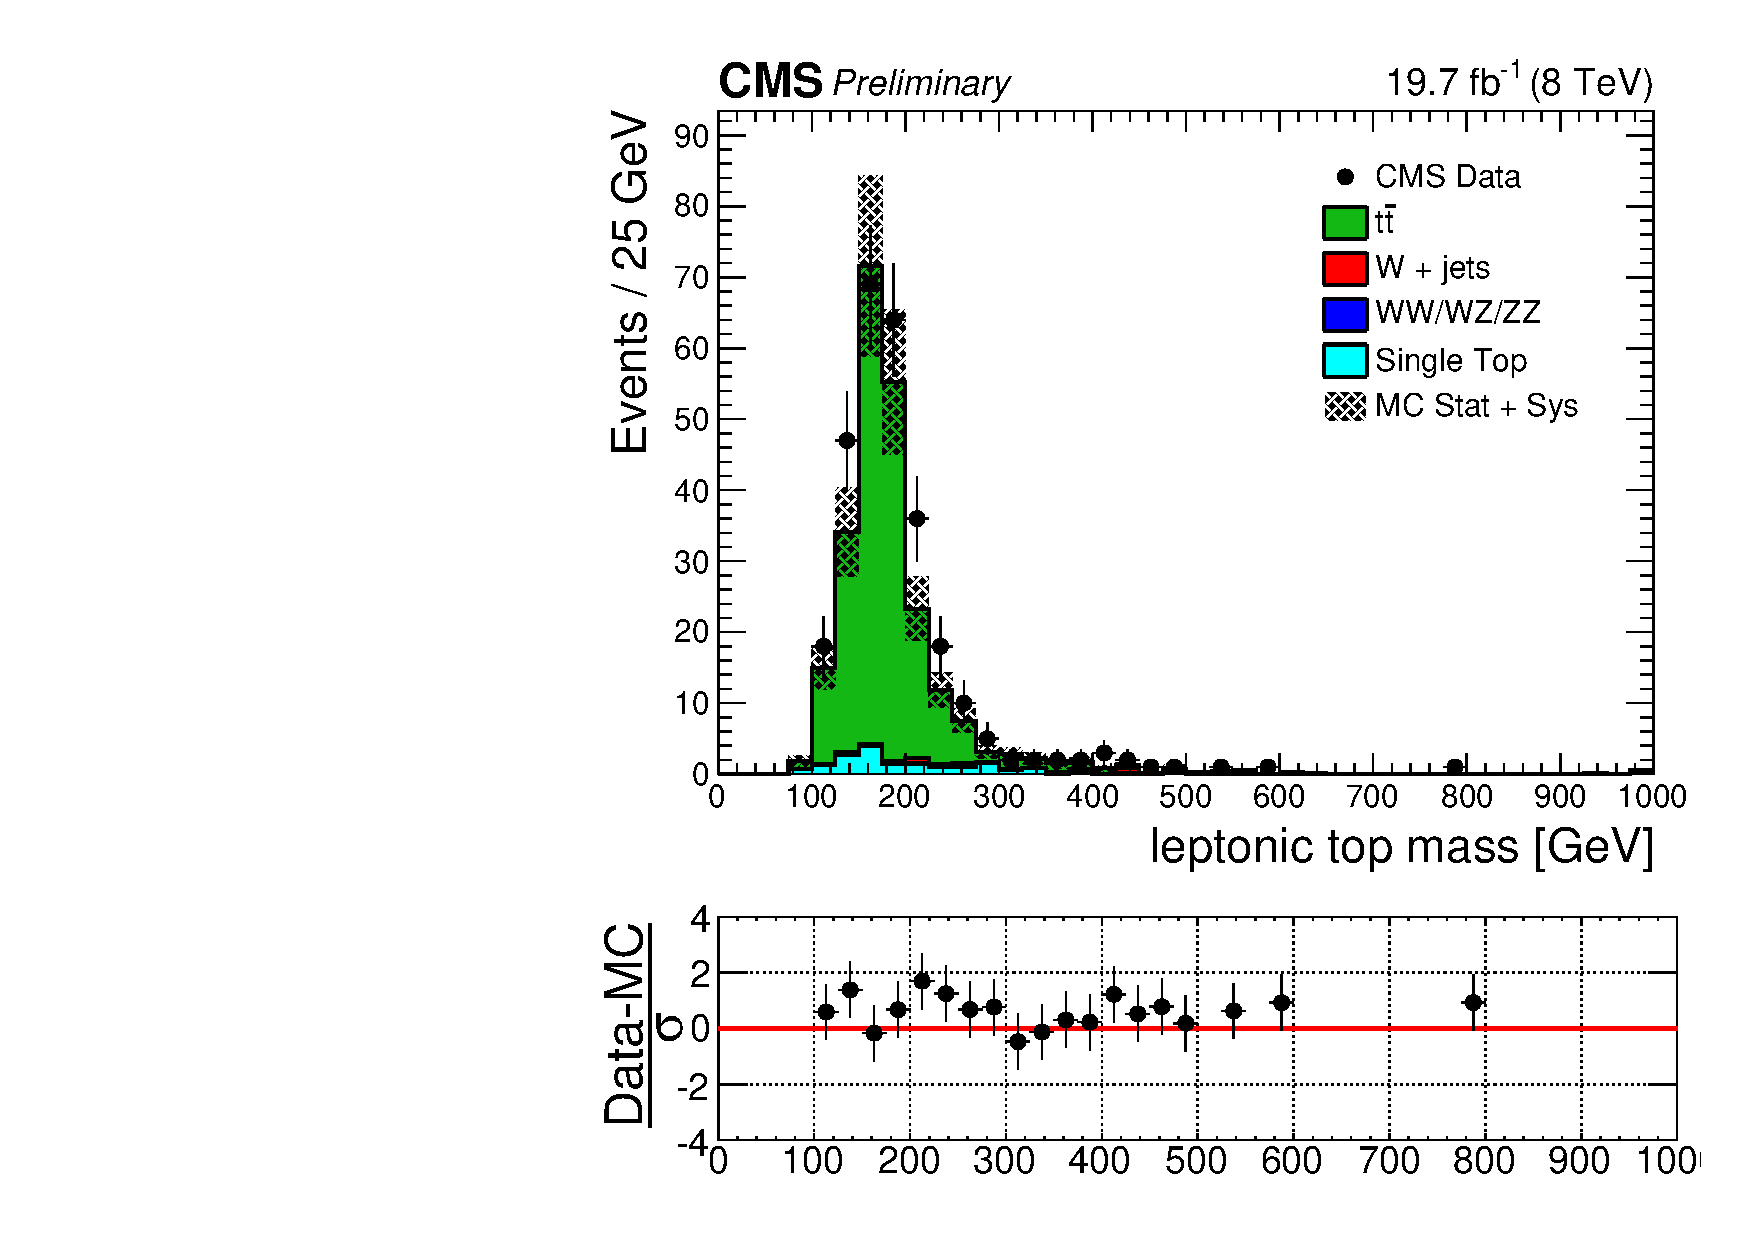
\includegraphics[width=0.45\textwidth]{\cheight/ttbar-mtoplept-mu-8TeV.pdf}}
\subfigure[]{\label{fig:tt-mtop8TeV_c}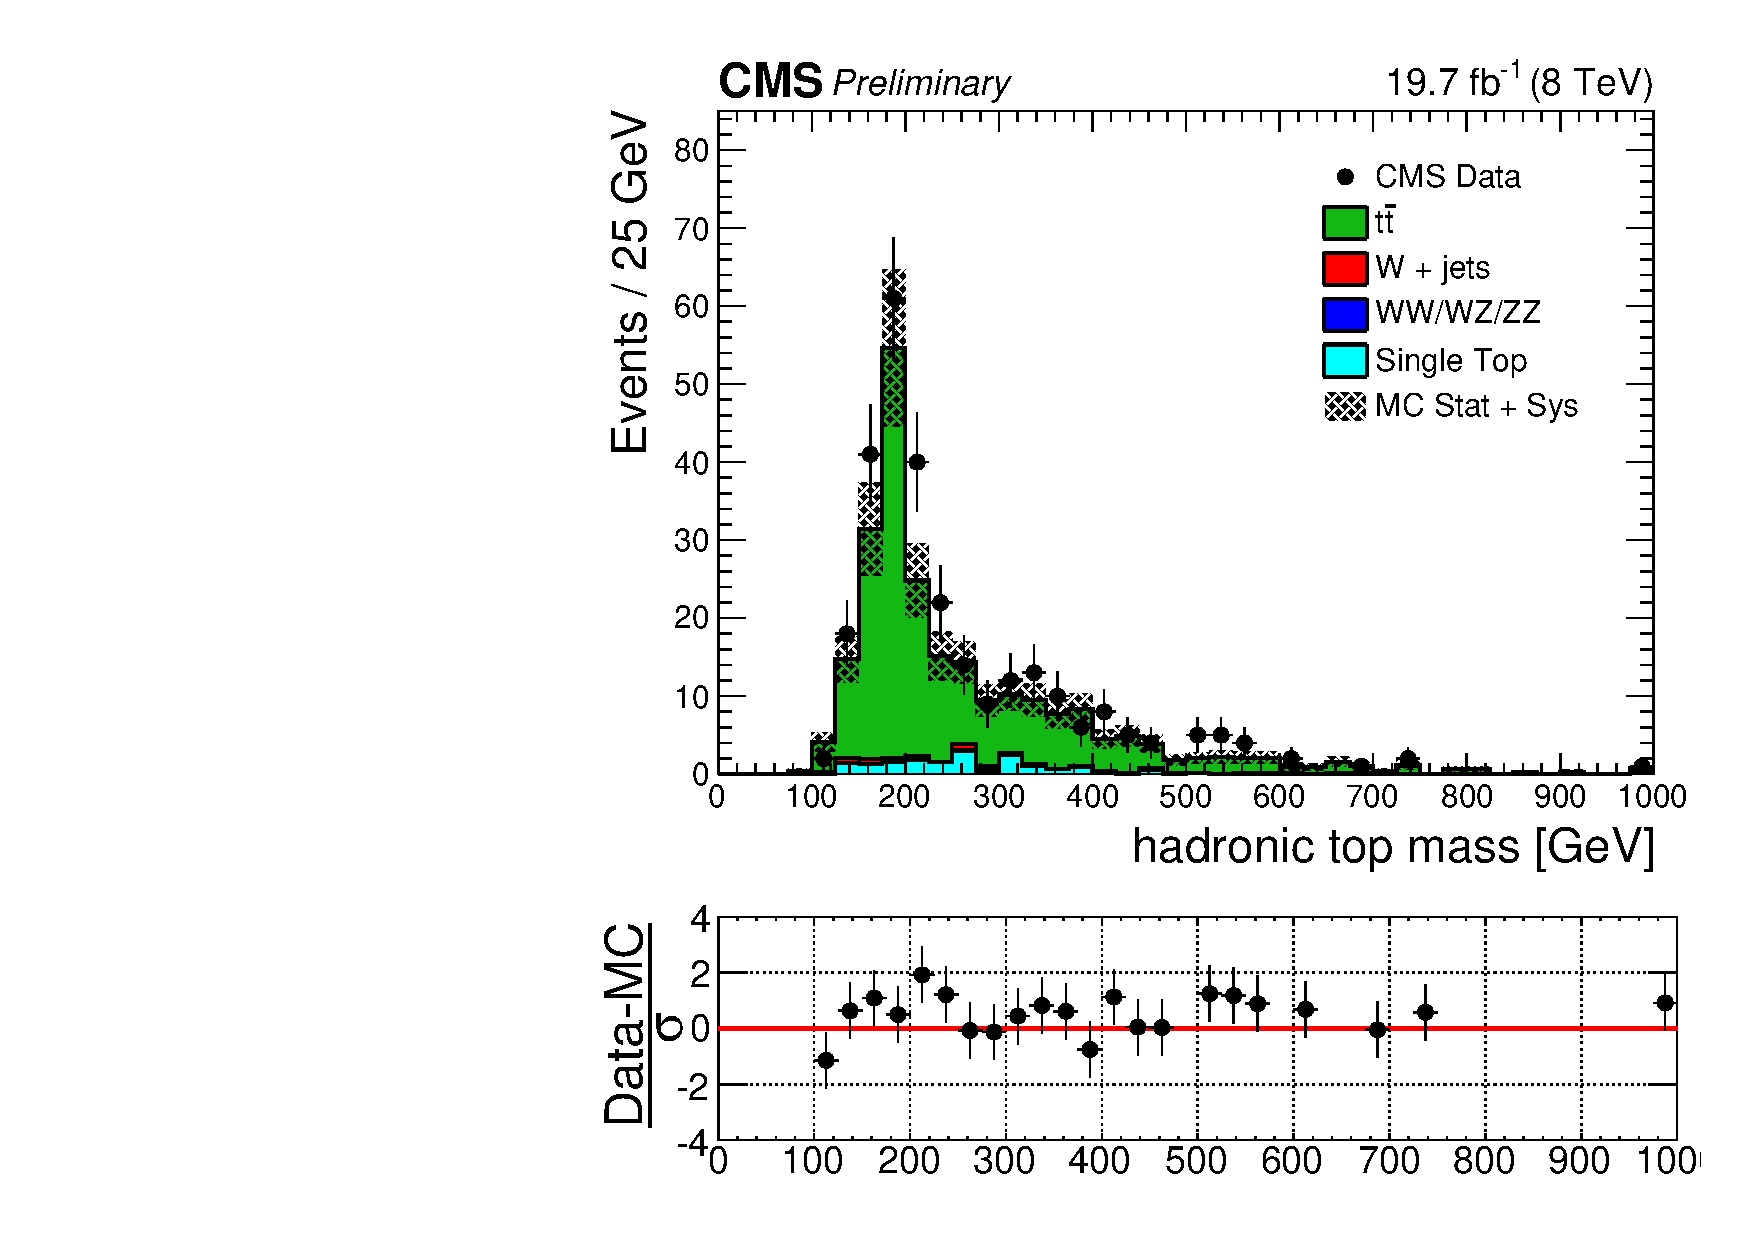
\includegraphics[width=0.45\textwidth]{\cheight/ttbar-mtophadr-mu-8TeV.pdf}}
\caption{Distributions for 8\TeV data and for simulation in \mWH (a), $m_\mathrm{top}^\mathrm{l}$ (b) and $m_\mathrm{top}^\mathrm{h}$ (c) in the top quark enriched control sample for the muon channel of the $\ell\Pgn\bbbar$ analysis.}
\label{fig:tt-mtop8TeV}
\end{figure}
 
%\section{Signal modeling}\label{sec:signalModel}
 %%%%%%%%%
\section{Signal modeling}\label{sec:signalModel}
%%%%%%%%%

The potential discovery and exclusion power of these analyses rely on the ability of finding a local enhancement on the top of a smoothly falling background. 
This is achieved through an unbinned likelihood fit of the signal + background model to the reconstructed diboson invariant mass, which depends on the accurate description of the signal shape.

An analytical parametrization of the signal shape is chosen such that it well reproduces the simulated resonance distributions.
As stated in Section~\ref{subsec:signalMC}, simulated signal events are generated with a resonance natural width sufficiently small compared to the detector resolution.
This makes the model used for generating the events dependent only on the detector effects on the signal shape, allowing a model independent search for narrow resonances
where only the detector resolution has to be described. A double-sided Crystal-Ball (CB) function~\cite{CrystalBallRef} (i.e. a Gaussian core with power law tails on both sides) is found to well serve this purpose.
To take into account differences between muon and electron momentum resolutions, the signal invariant mass distribution is parametrized separately in the two lepton flavor categories.

Figure~\ref{fig:mWVfit-signal-13TeV} shows examples of the fitted signal distribution through a CB function, for several signal benchmarks and in different \mJ categories of the $\ell\nu\qqbar$ analysis.
Similar results are obtained for the \Wpr signal used in the $\ell\nu\bbbar$ analysis.
%an example for the fitted signal distribution through a CB function for a \Wpr mass of 1.5\TeV in the muon channel of the $\ell\nu$+H-jet analysis.
%Other examples are shown in Fig.~\ref{fig:mWVfit-signal-13TeV}, for the $\ell\nu$+V-jet analysis in the muon channel, for several signal hypotheses and for both \mJ categories.

%\begin{figure}[!htb]
%\centering
%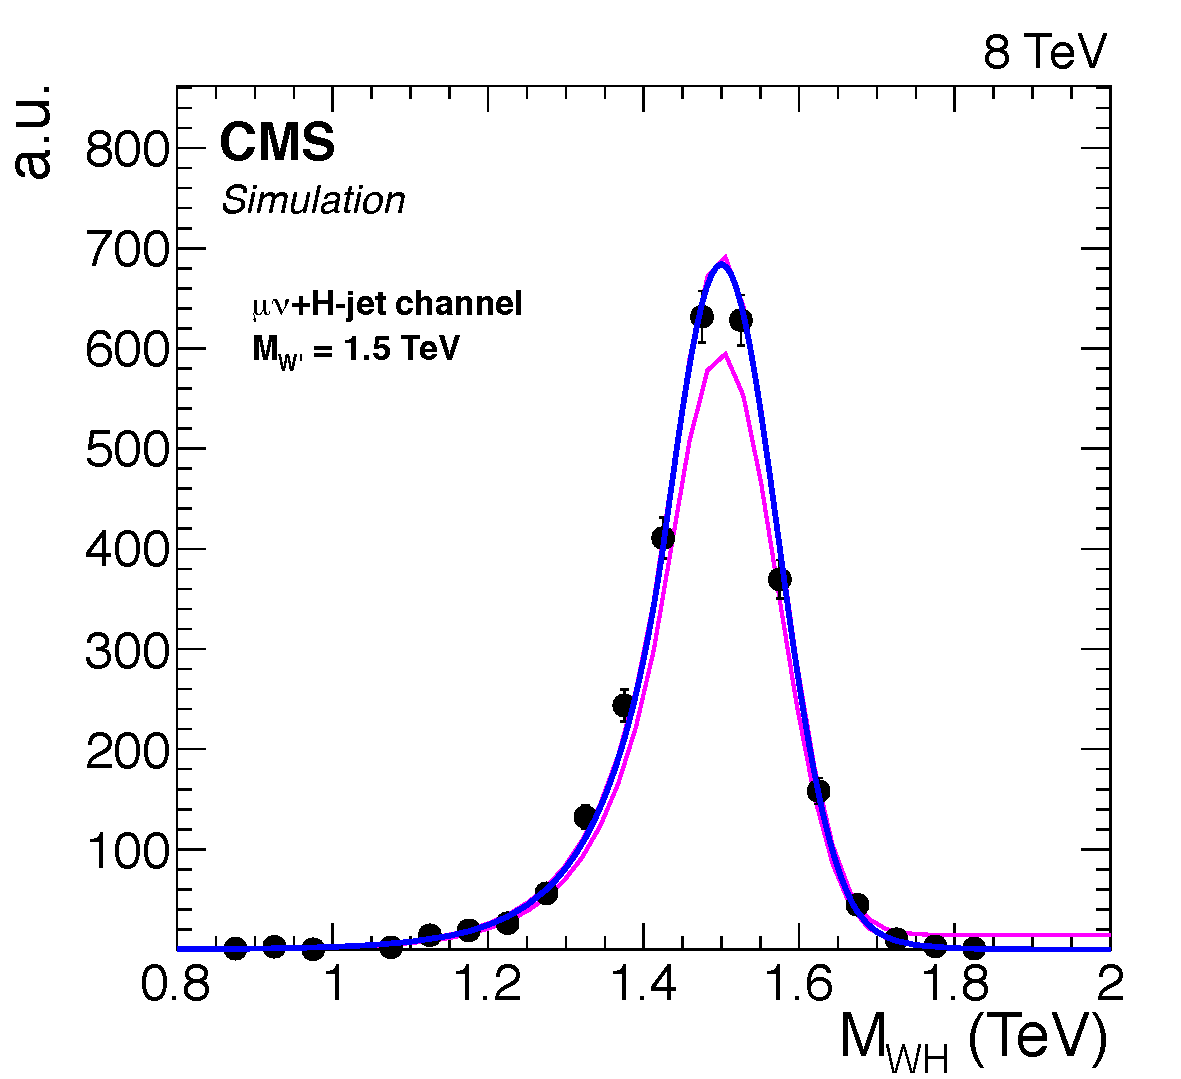
\includegraphics[width=0.5\textwidth]{\cheight/mWH-signal-mu-8TeV.pdf}
%\caption{blabla}
%\label{fig:mWHfit-signal-8TeV}
%\end{figure}

\begin{figure}[!htb]
\centering
\subfigure[]{\label{fig:mWVfit-signal-13TeV_a}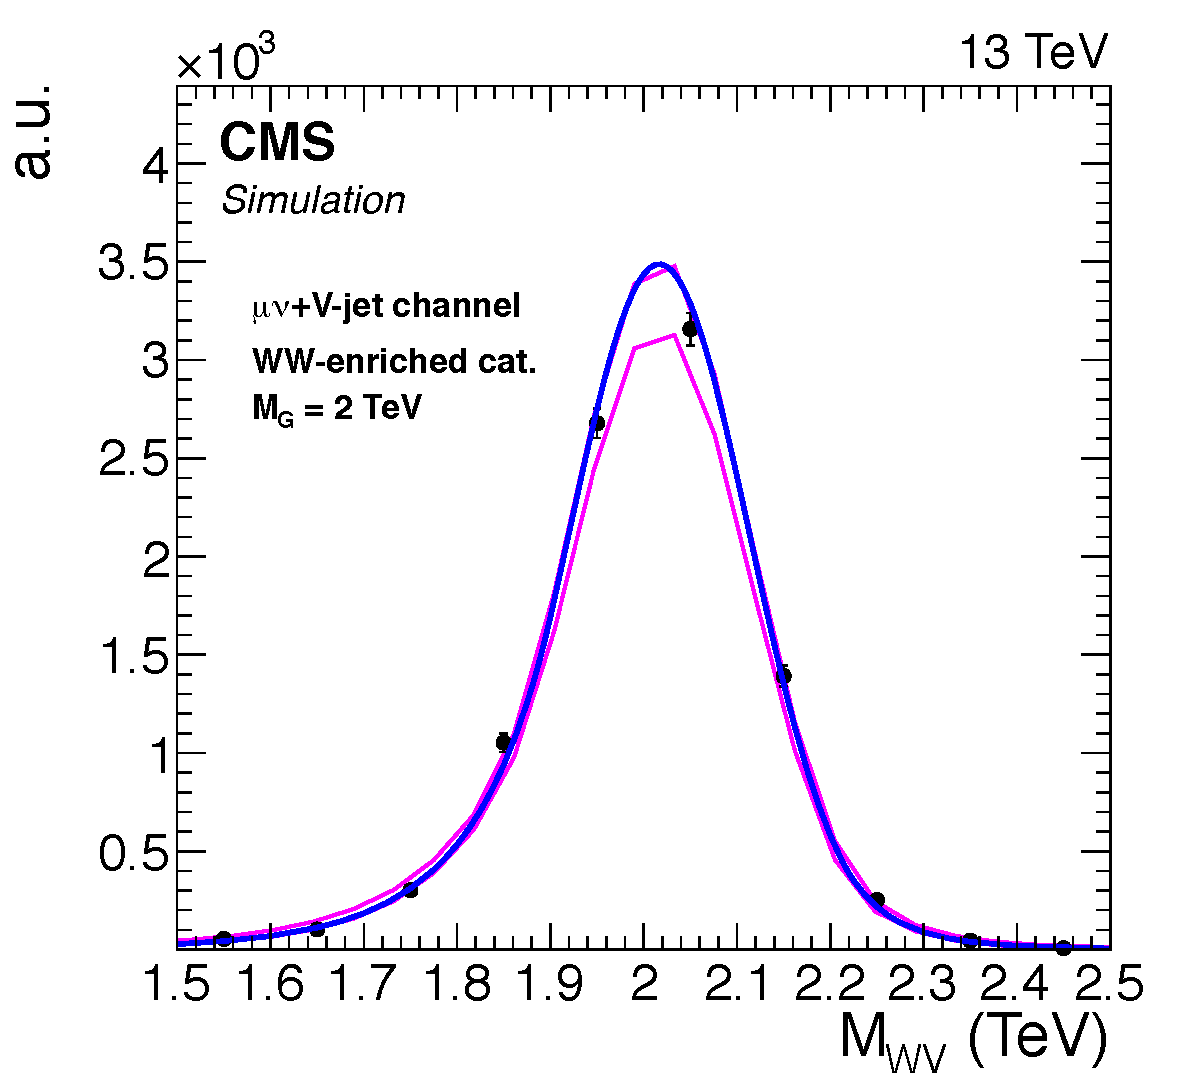
\includegraphics[width=0.3\textwidth]{\cheight/mWV-signal-bulkg-mu-HPW-13TeV.pdf}}
\subfigure[]{\label{fig:mWVfit-signal-13TeV_b}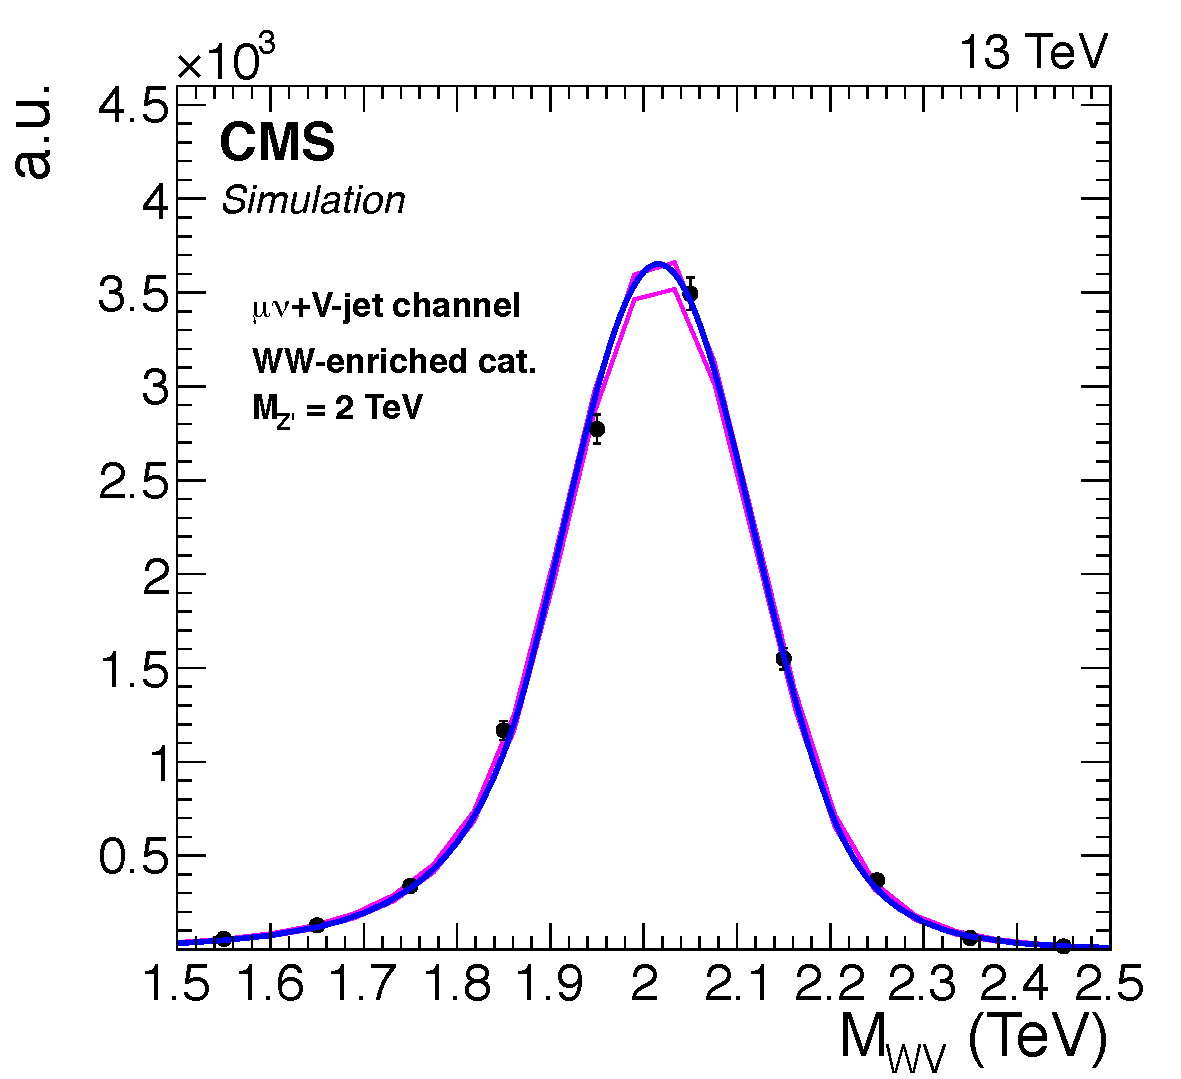
\includegraphics[width=0.3\textwidth]{\cheight/mWV-signal-zprime-mu-HPW-13TeV.pdf}}
\subfigure[]{\label{fig:mWVfit-signal-13TeV_c}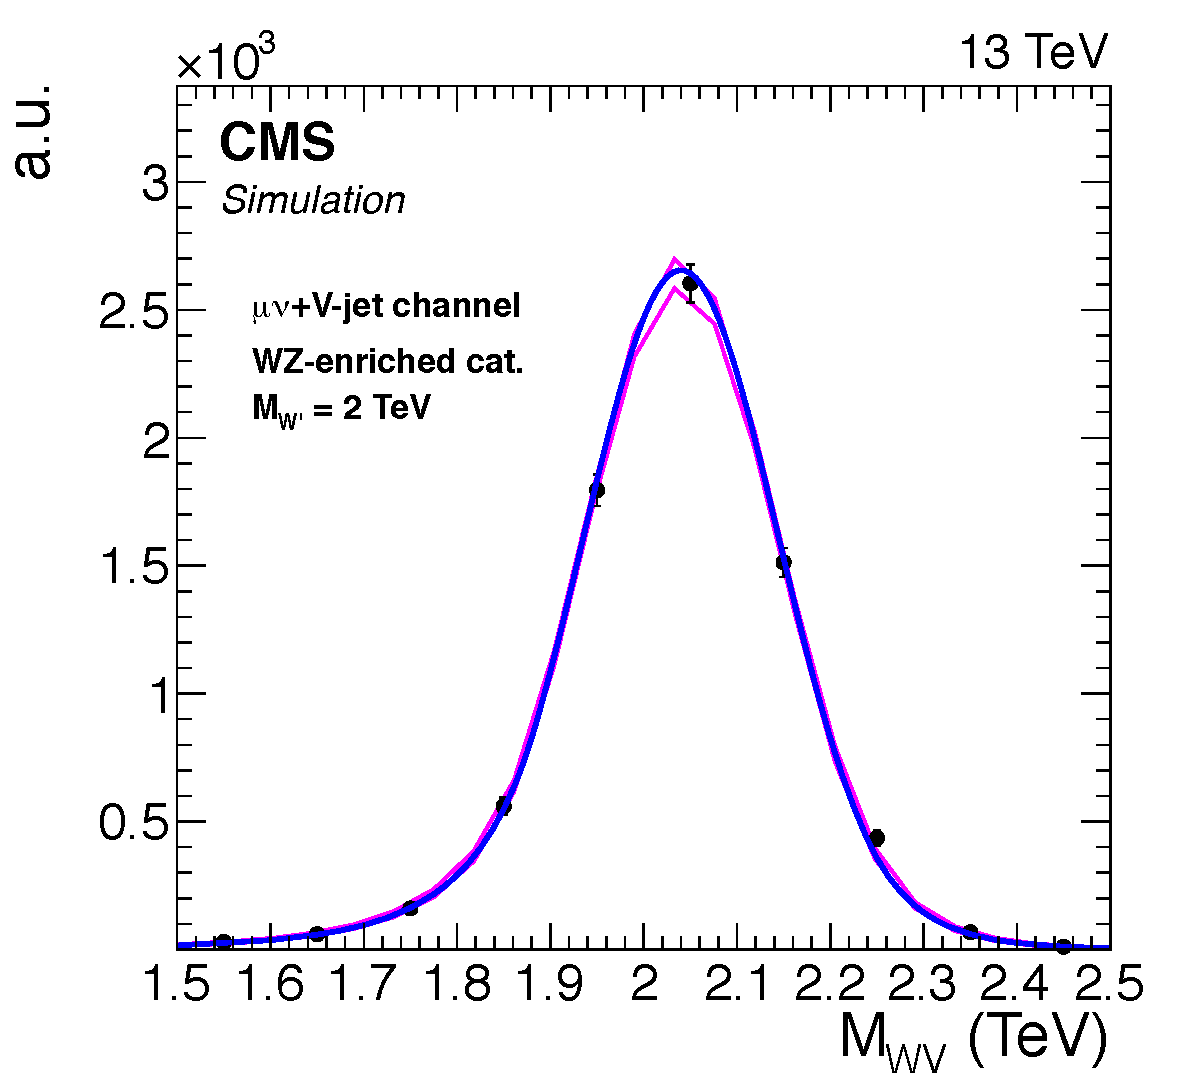
\includegraphics[width=0.3\textwidth]{\cheight/mWV-signal-wprime-mu-HPZ-13TeV.pdf}}
\caption{Modeling of the reconstructed signal distribution with a double-sided Crystal Ball function, for different signal benchmarks and in different \mJ categories of the $\ell\nu\qqbar$ analysis: 
bulk graviton (a) and \Zpr (b) signals in the WW-enriched category; (c) \Wpr signal in the WZ-enriched category. In all cases, a signal sample with a generated mass of 2\TeV is considered.}
\label{fig:mWVfit-signal-13TeV}
\end{figure}

Because of the limited number of available simulated samples, a linear interpolation is performed for each parameter of the CB function between
the shapes obtained for some reference mass points, in order to extrapolate the distribution for intermediate values of the resonance mass.
The resolution of the reconstructed diboson invariant mass is given by the width of the Gaussian core and it ranges between 7 and 4\% depending on the resonance mass, as summarized in Fig.~\ref{fig:relCB}.
The resolution is dominated by the jet and \ETmiss contributions.

\begin{figure}[!htb]
\centering
\subfigure[]{\label{fig:relCB_a}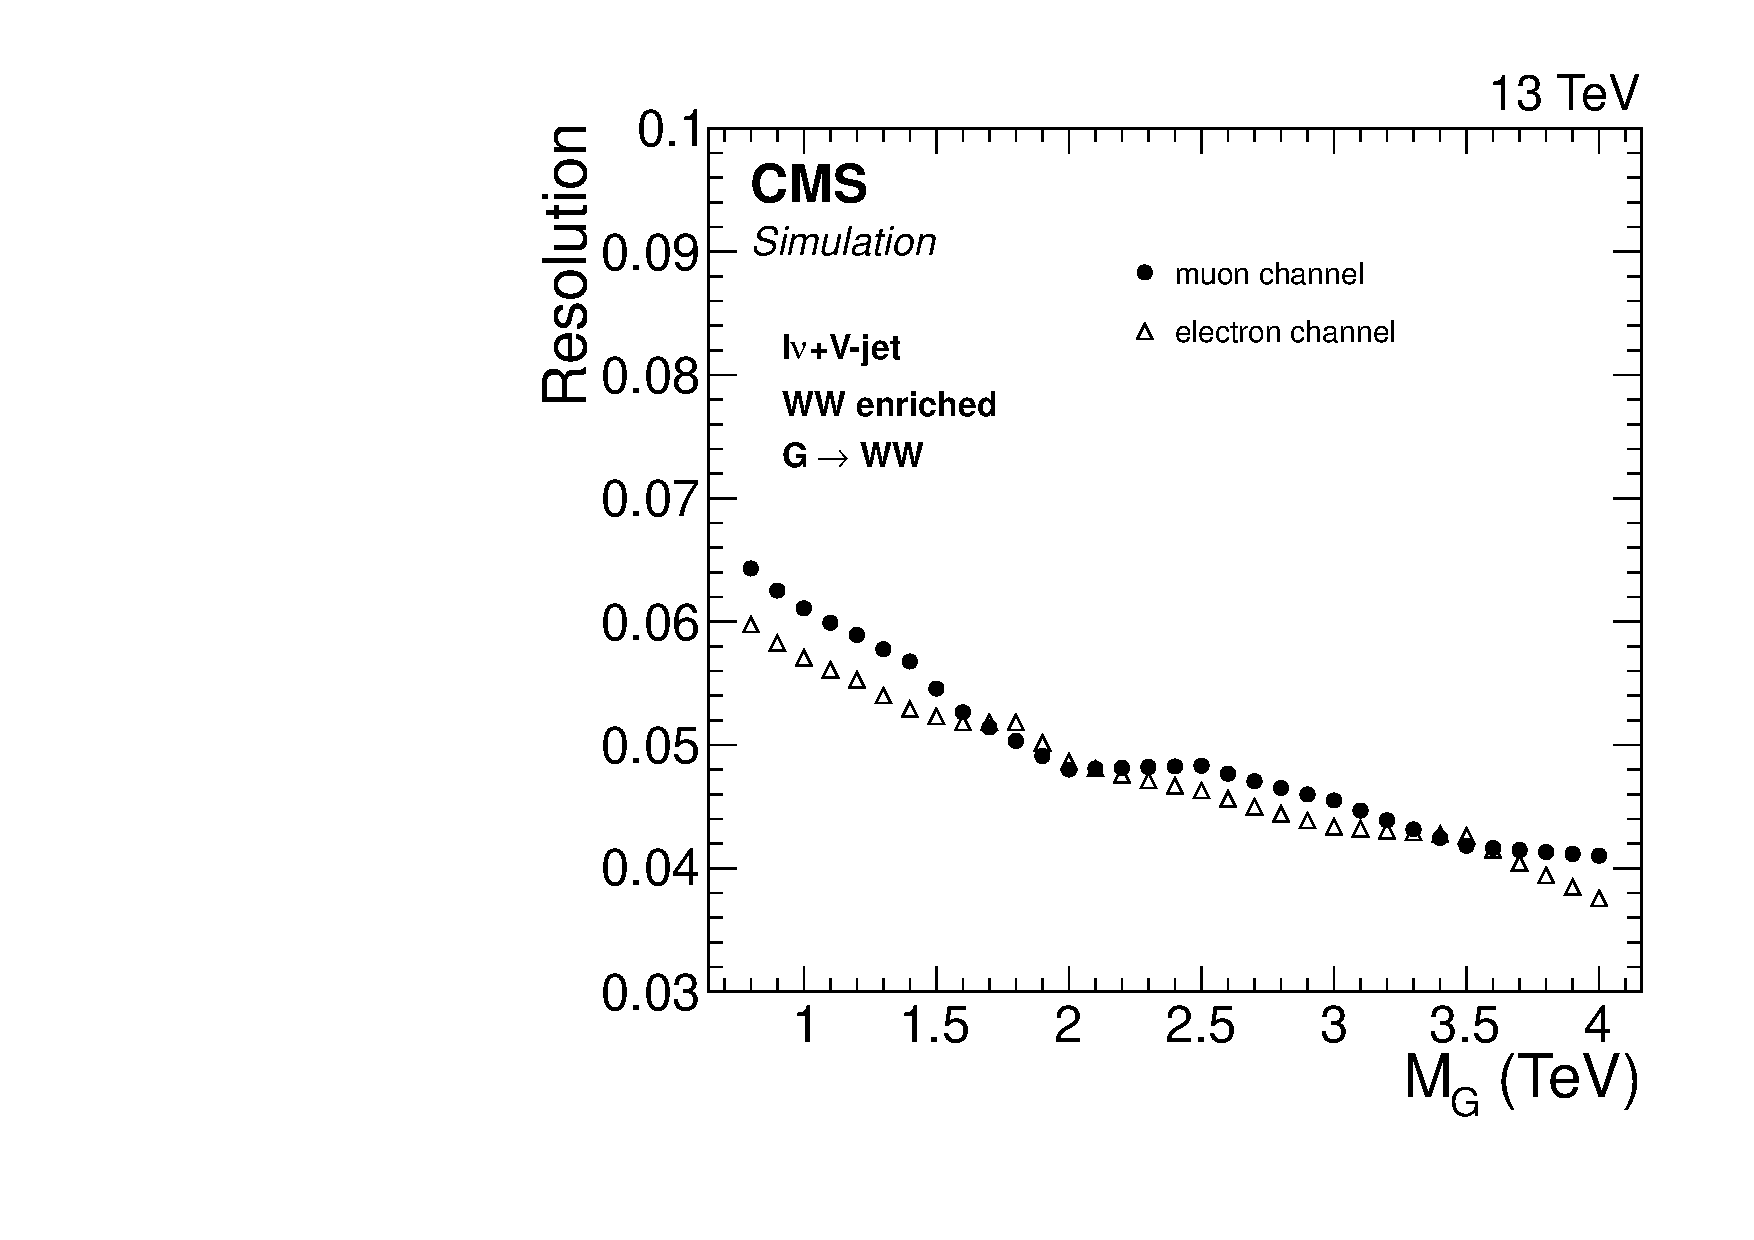
\includegraphics[width=0.3\textwidth]{\cheight/CBrel-bulkg-HPW-13TeV.pdf}}
\subfigure[]{\label{fig:relCB_b}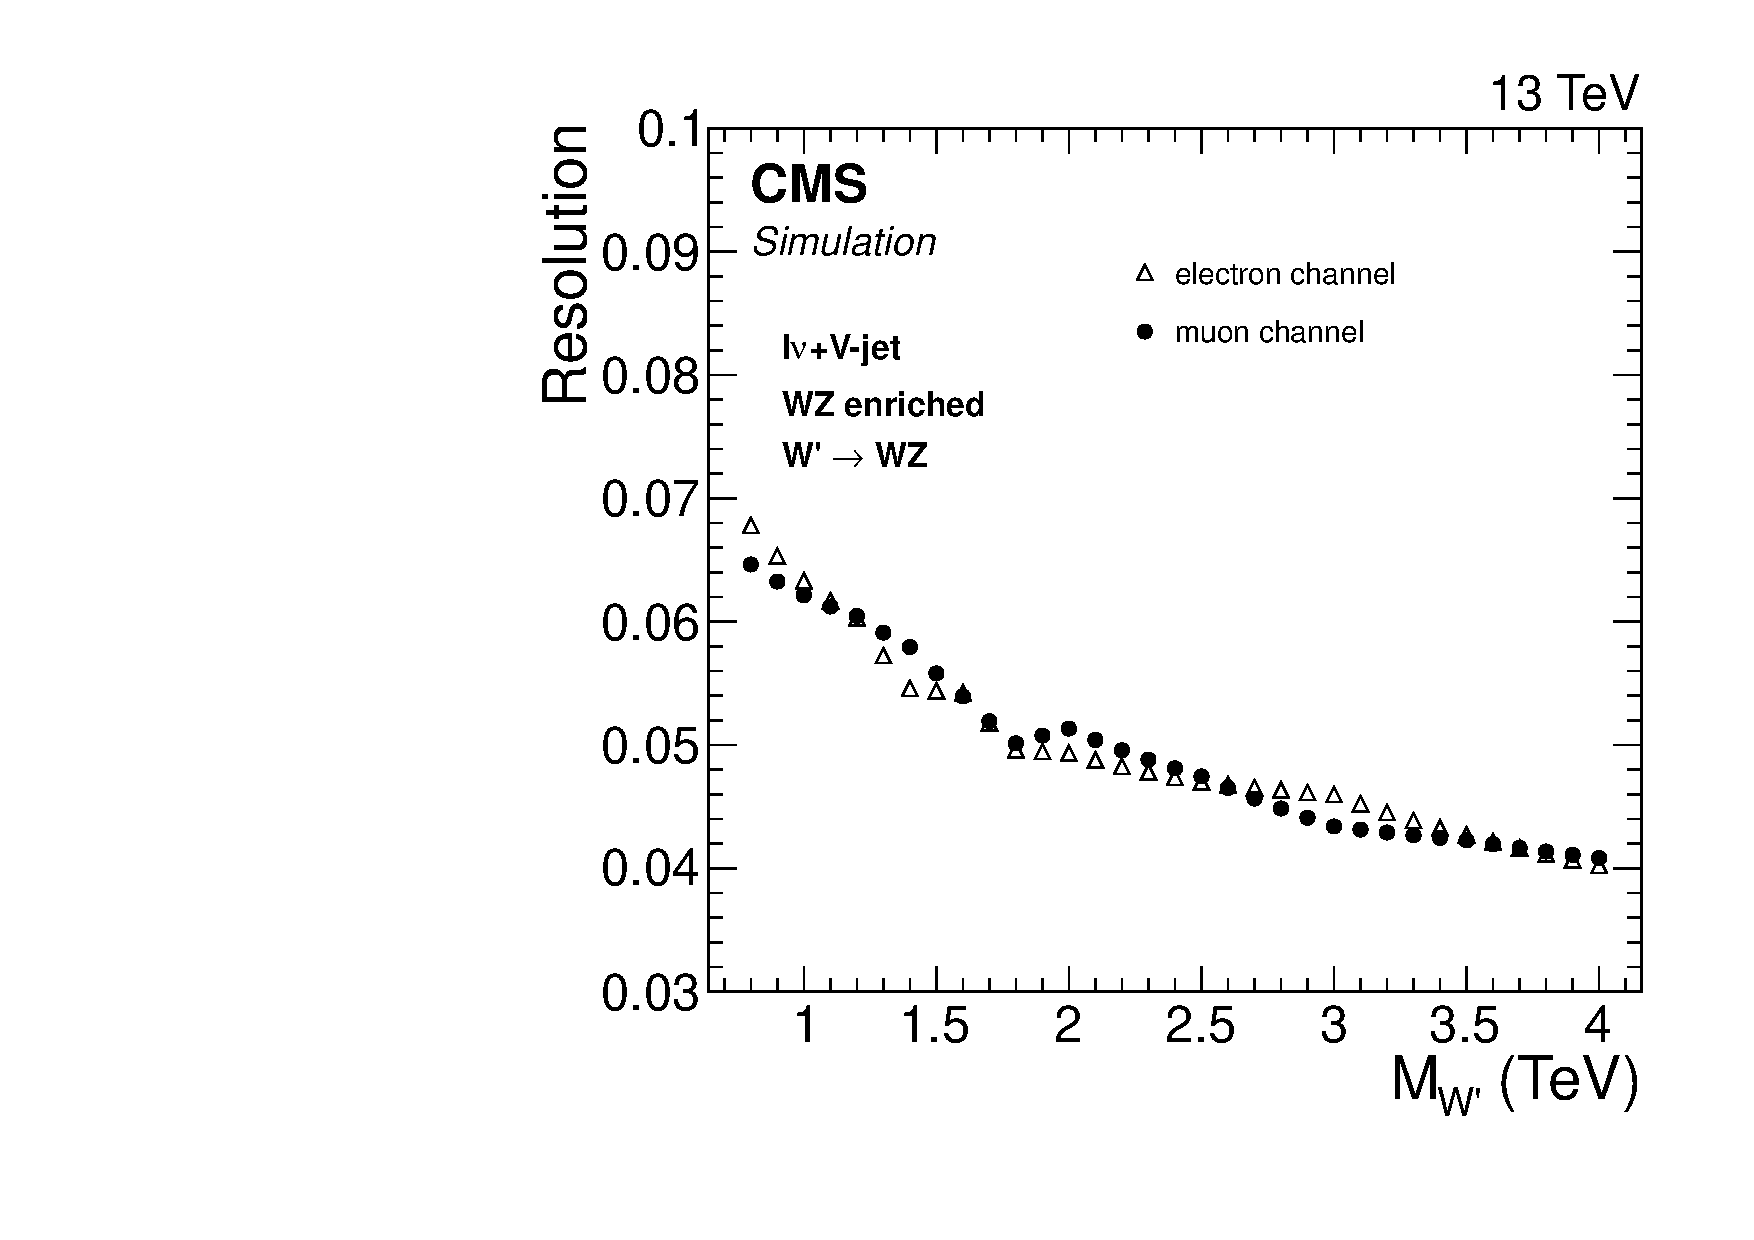
\includegraphics[width=0.3\textwidth]{\cheight/CBrel-wprime-HPZ-13TeV.pdf}}
\subfigure[]{\label{fig:relCB_c}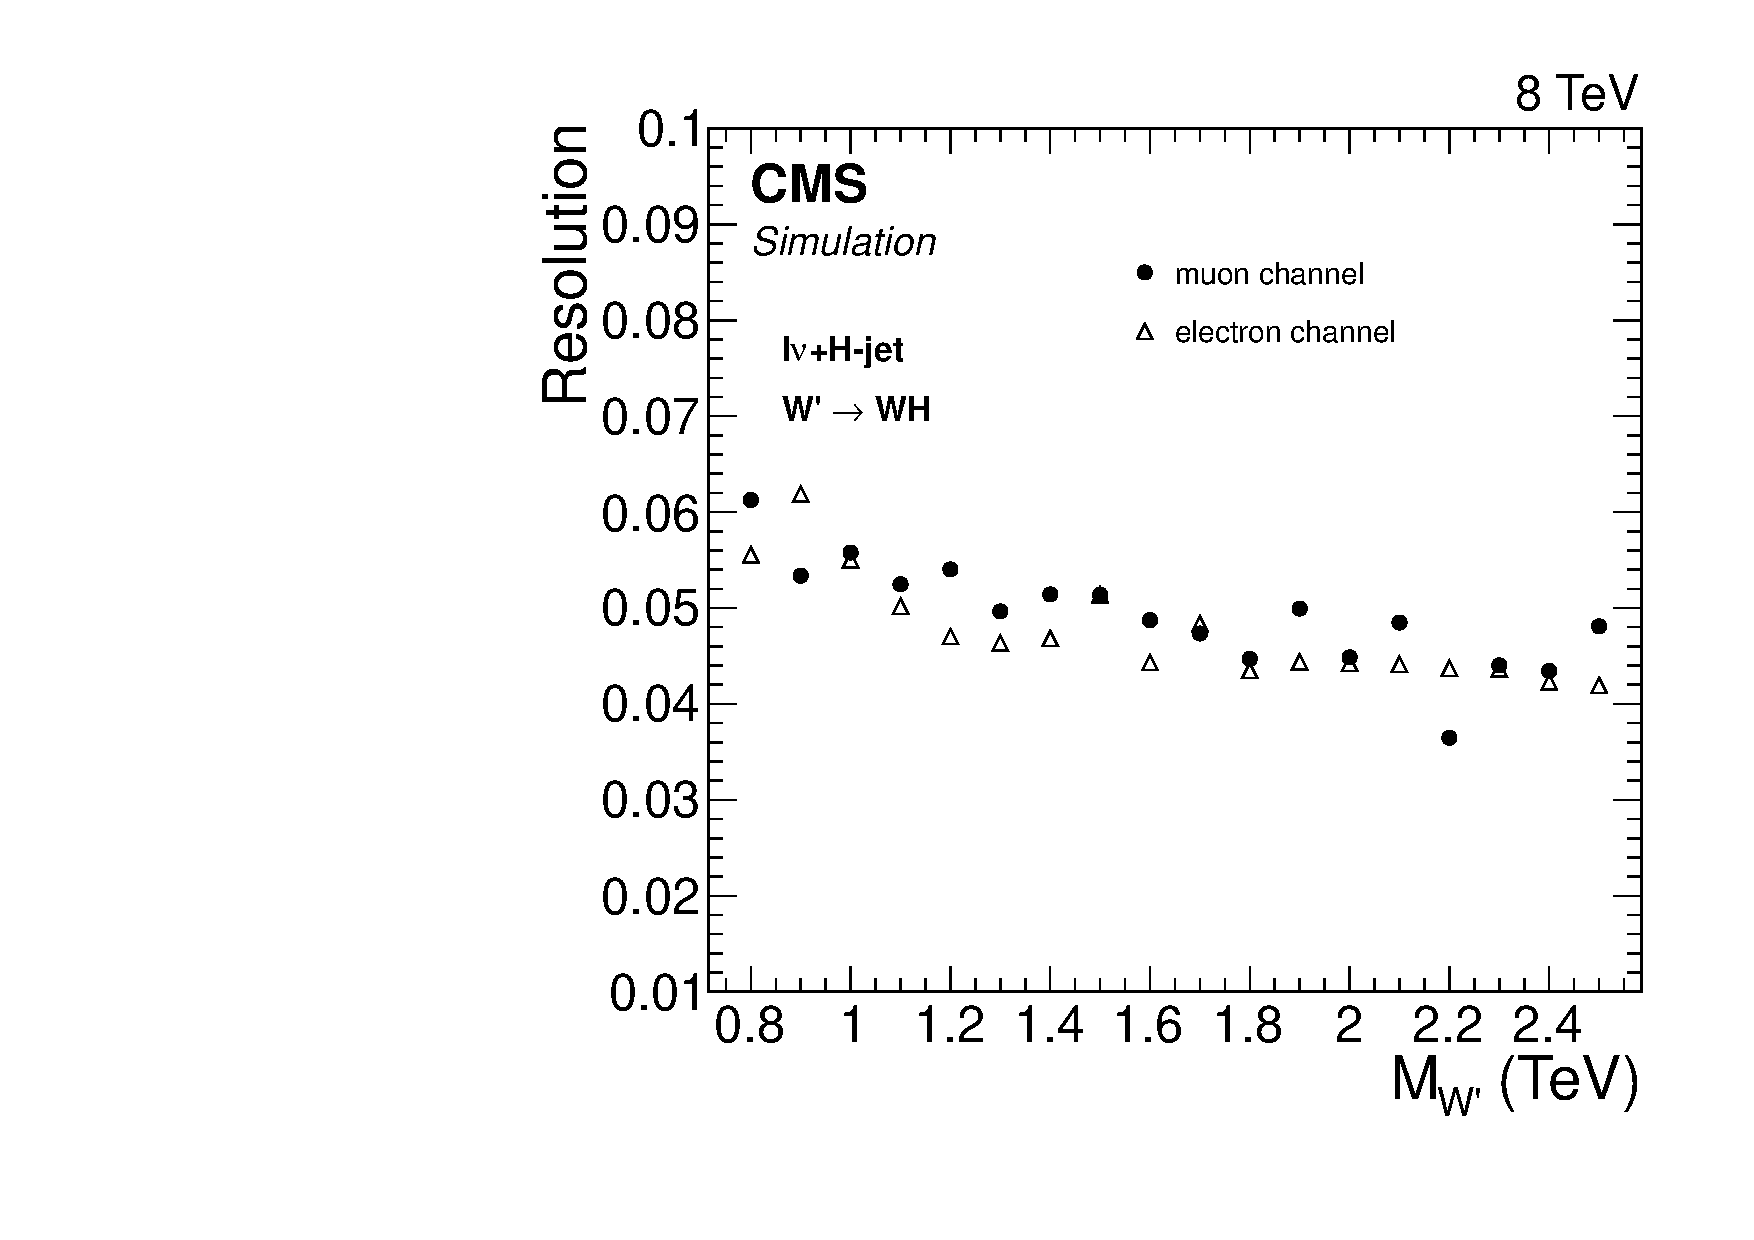
\includegraphics[width=0.3\textwidth]{\cheight/CBrel-wprime-WH-8TeV.pdf}}
\caption{Relative resolution of the fitted signal distribution as given by the width of the Gaussian core, as a function of the generated resonance mass for different signal benchmarks and for the two analysis:
bulk graviton (a) and \Wpr (b) signals in the WW-enriched and WZ-enriched category, respectively, of the $\ell\nu\qqbar$ analysis; (c) \Wpr signal for the $\ell\nu\bbbar$ analysis.}
\label{fig:relCB}
\end{figure}

The signal selection efficiency, evaluated for each category, is defined as the number of selected signal events over the number of generated ones, which include all the possible lepton flavours (e, $\mu$ and $\tau$).
As shown in Fig.~\ref{fig:effWV-13TeV} the efficiency for a $\Zpr$ or bulk graviton signal in the WW-enriched category is $\approx$ 2 times larger compared to a $\Wpr$ signal. On the other hand, the efficiency for a $\Wpr$ signal in the WZ-enriched category is $\approx$ 4 times larger compared to a $\Zpr$ or bulk graviton signal. For both categories and for each signal hypothesis the efficiency is smaller compared to the large \mJ window used for V tagging. However, the resulting loss in sensitivity in each of the category is recovered with a combination of the two \mJ categories which allows the use of all the available data. With this solution the discrimination between the two type of signals is maximized together with a gain in sensitivity of 10--20\% depending on the resonance mass.

A linear interpolation of the signal efficiency is performed between the values obtained for some reference mass points in order to extrapolate the efficiency for intermediate resonance masses for which a simulated sample is not available.
The efficiency for the electron channel is lower compared to the muon channel over most of the phase space due to the tighter requirements on the electron \pt and \ETmiss. This effect is less visible in the $\ell\Pgn\bbbar$ channel (Fig.~\ref{fig:effWH-8TeV}) where the electron selections are less strict. For all cases, at low masses the efficiency increases with the resonance mass because of the increase in the acceptance of the lepton, \ETmiss and $m_\mathrm{WV/WH}$ selections together with the inefficiency of the jet algorithms in reconstructing the merged jet for a low boosted V boson (Fig.~\ref{fig:ca8effVsPt}). At larger resonance masses the efficiency slightly decreases due to \nsubj selection inefficiency for very high \pt V jets, as described in Section~\ref{sec:vtagging}.
For the electron channel this effect is compensated by a larger increase in the lepton selection acceptance, resulting in a nearly flat efficiency at high resonance masses.
Similar considerations hold for the efficiency in the $\ell\Pgn\bbbar$ channel shown in Fig.~\ref{fig:effWH-8TeV}.

\begin{figure}[!htb]
\centering
\subfigure[]{\label{fig:effWV-13TeV_a}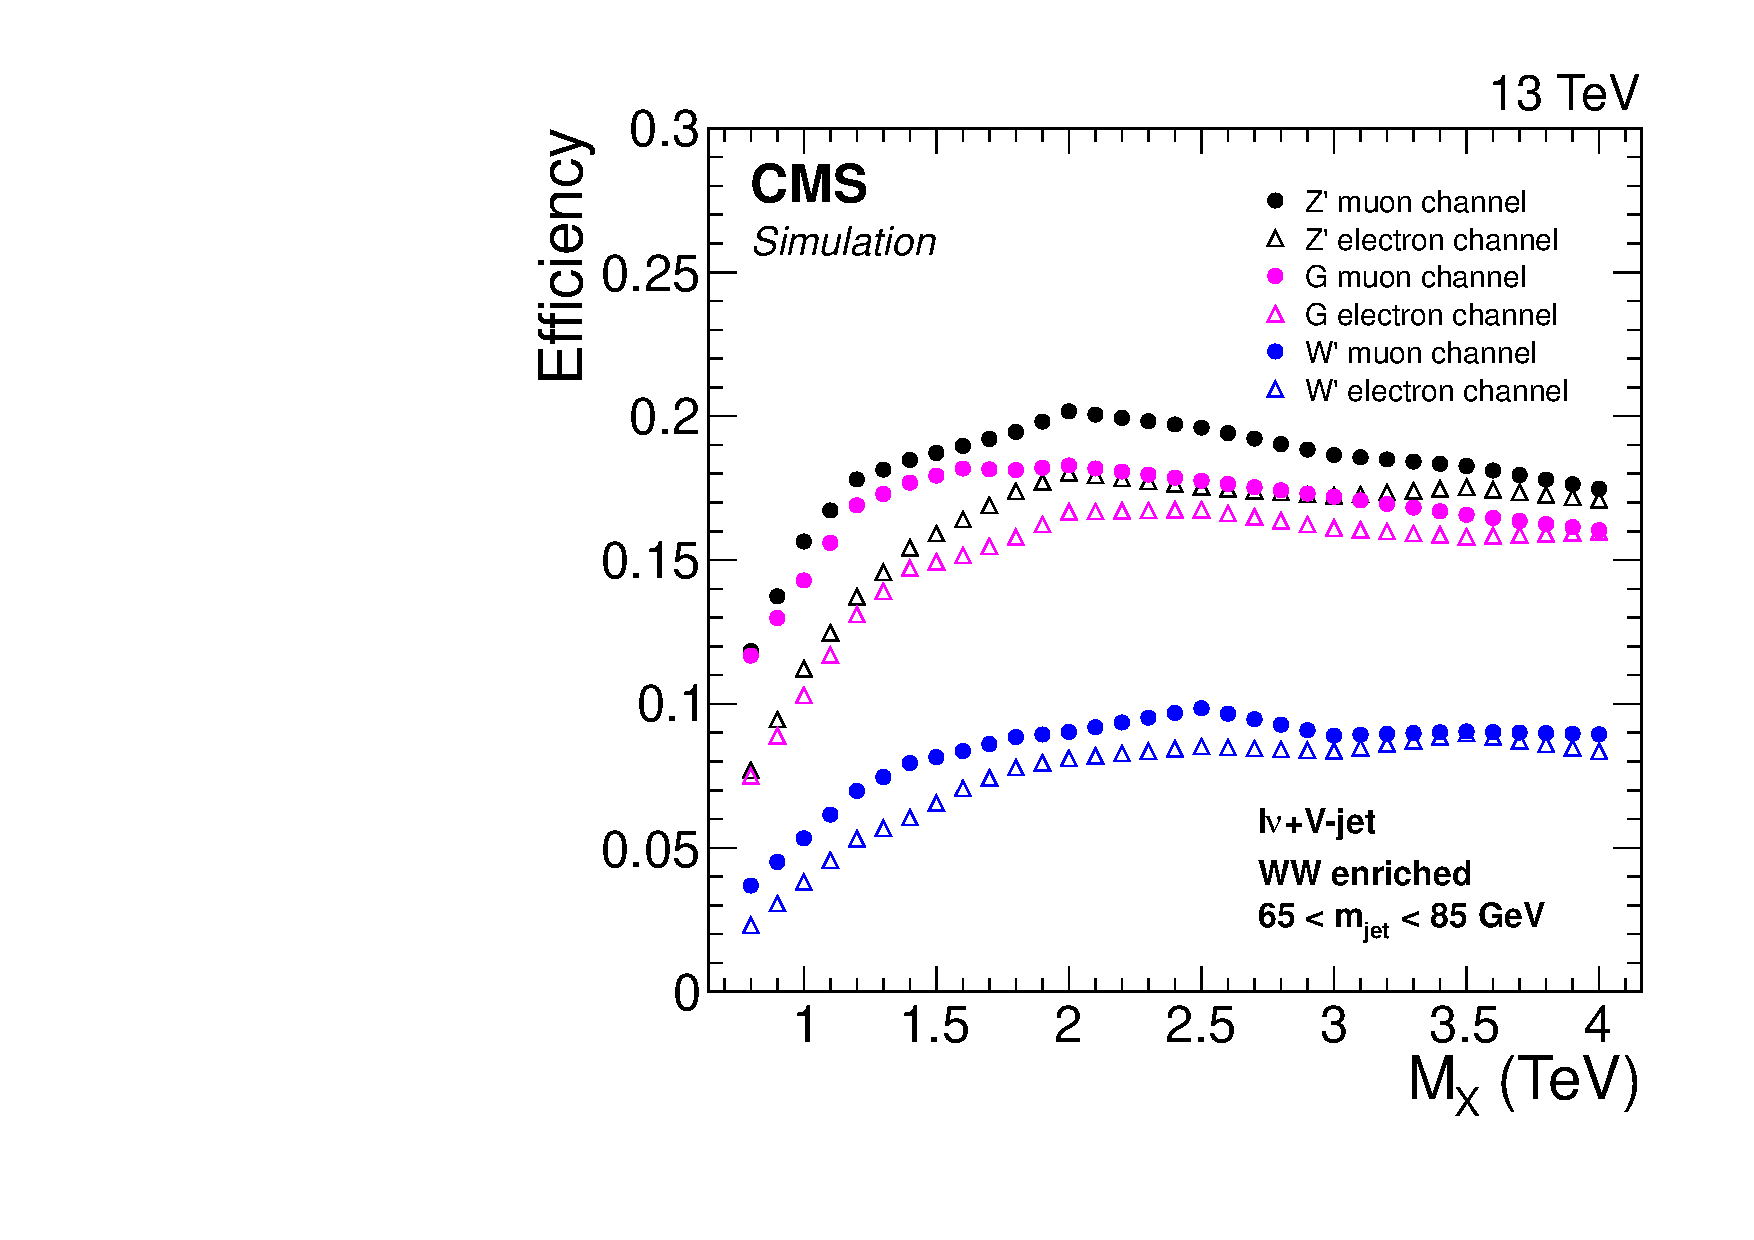
\includegraphics[width=0.3\textwidth]{\cheight/signal-eff-HPW-all.pdf}}
\subfigure[]{\label{fig:effWV-13TeV_b}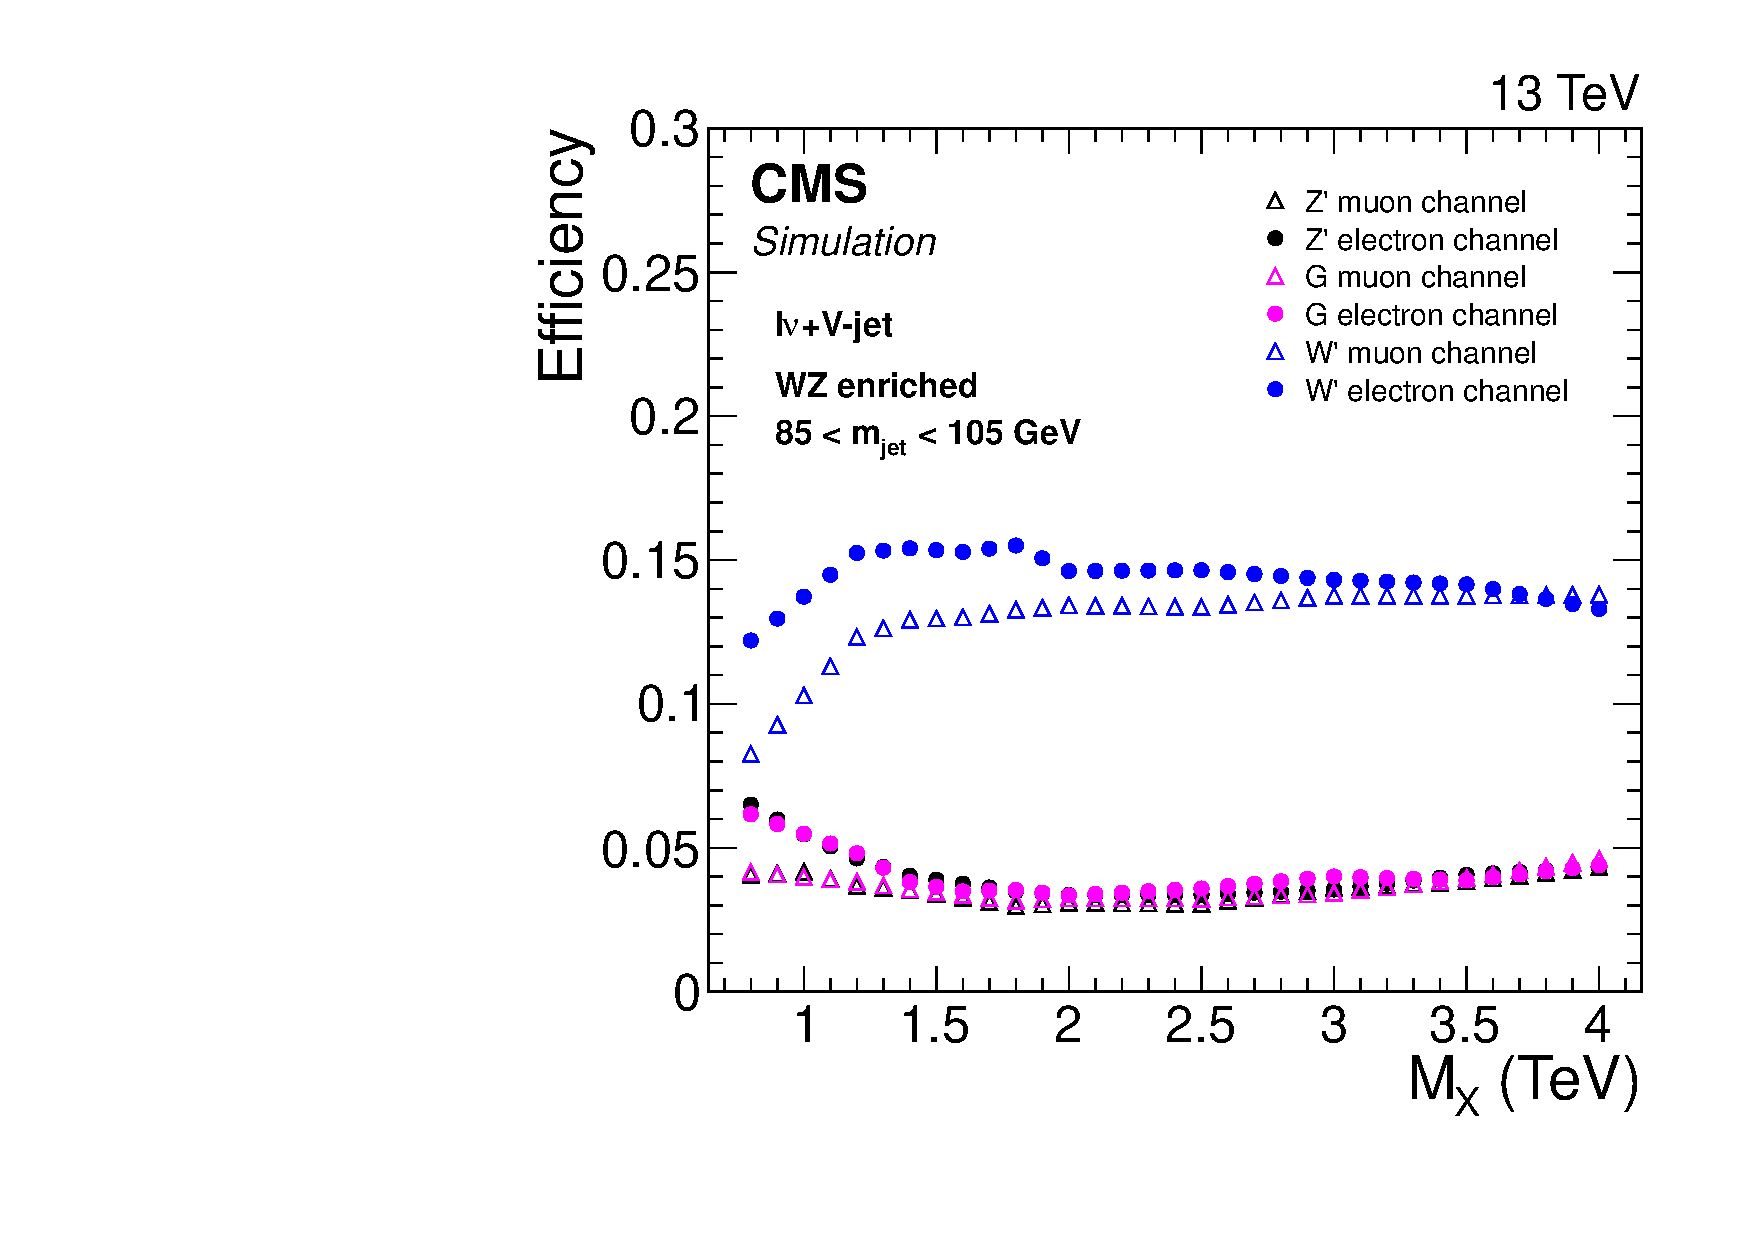
\includegraphics[width=0.3\textwidth]{\cheight/signal-eff-HPZ-all.pdf}}
\subfigure[]{\label{fig:effWV-13TeV_c}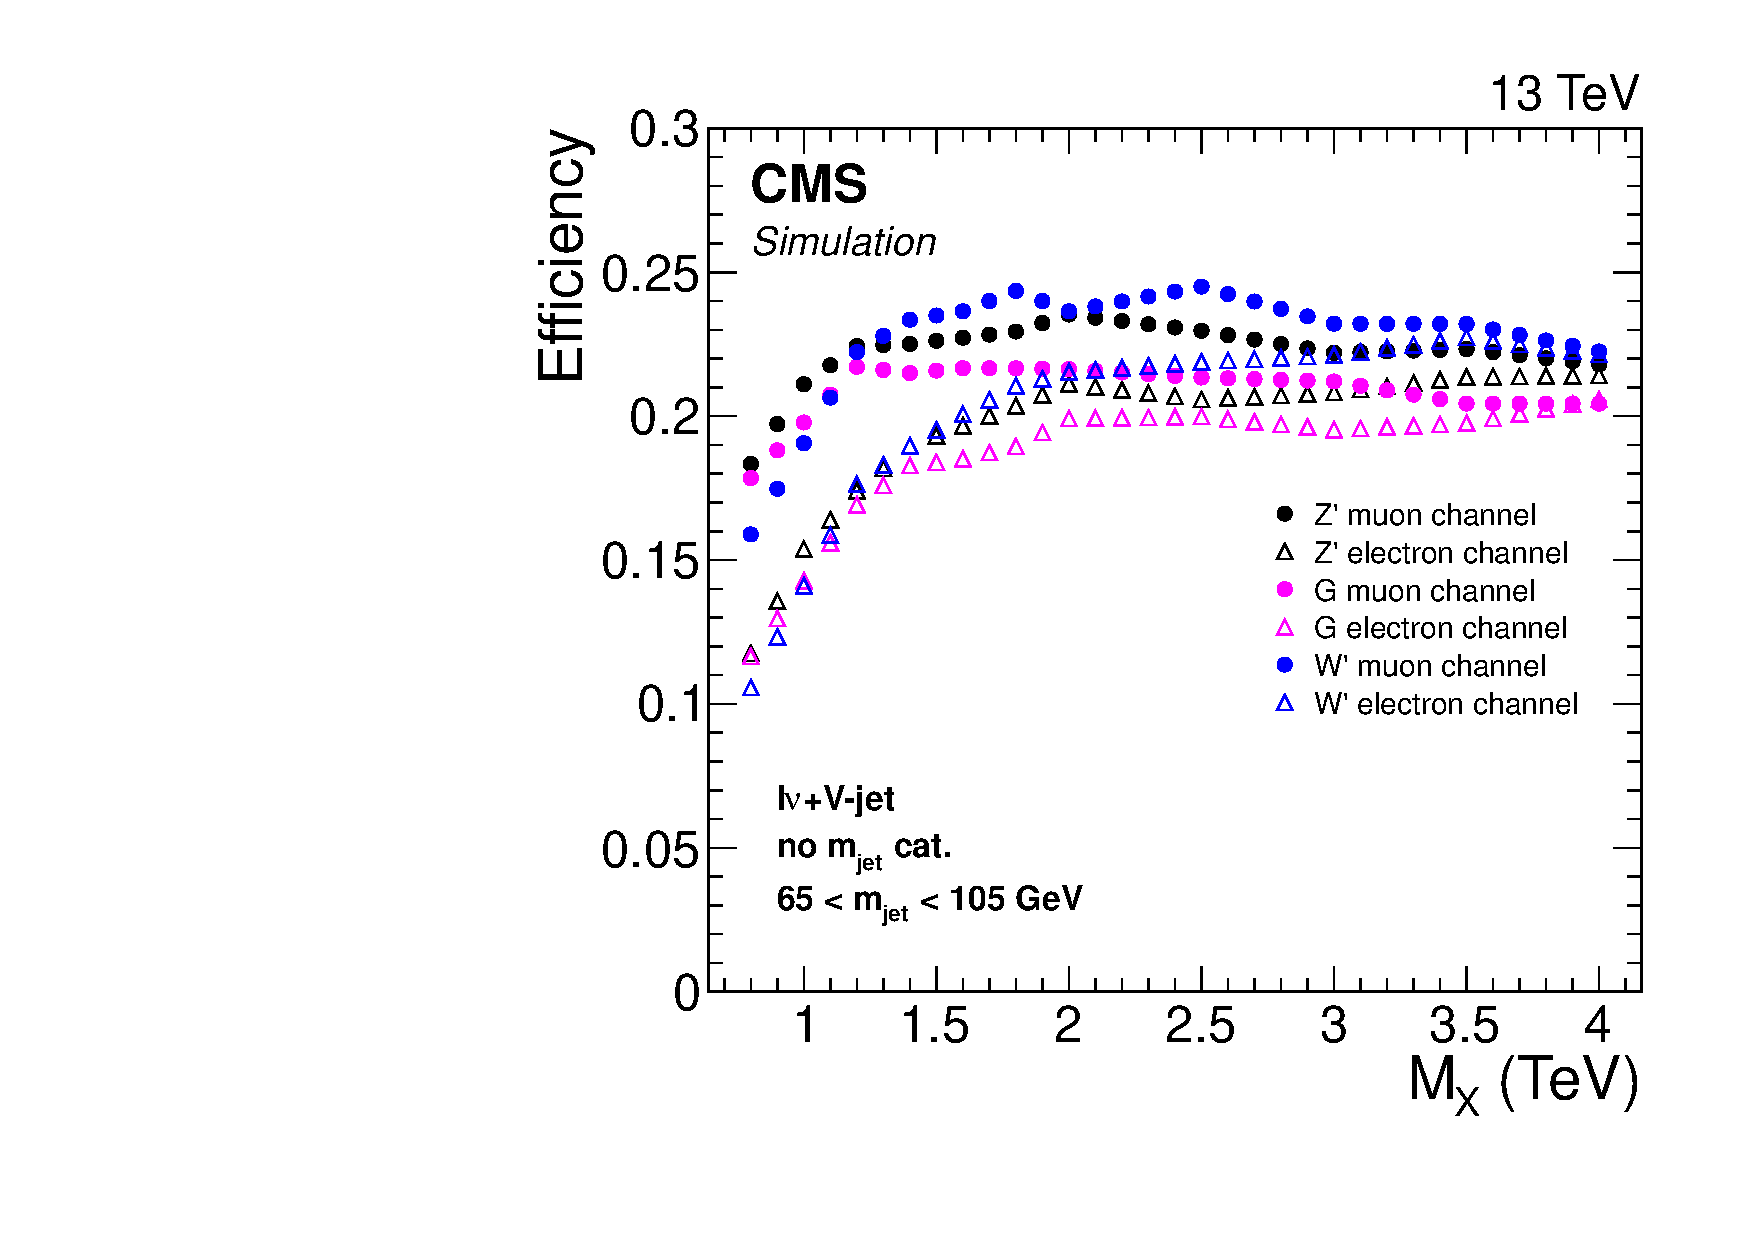
\includegraphics[width=0.3\textwidth]{\cheight/signal-eff-HP-all.pdf}}
\caption{Signal efficiency in the $\ell\nu\qqbar$ analysis channel as a function of the generated resonance mass for all signal benchmarks and for different \mJ selection: (a) WW-enriched category; (b) WZ-enriched category; (c) $65 < \mJ < 105\GeV$.}
\label{fig:effWV-13TeV}
\end{figure}

\begin{figure}[!htb]
\centering
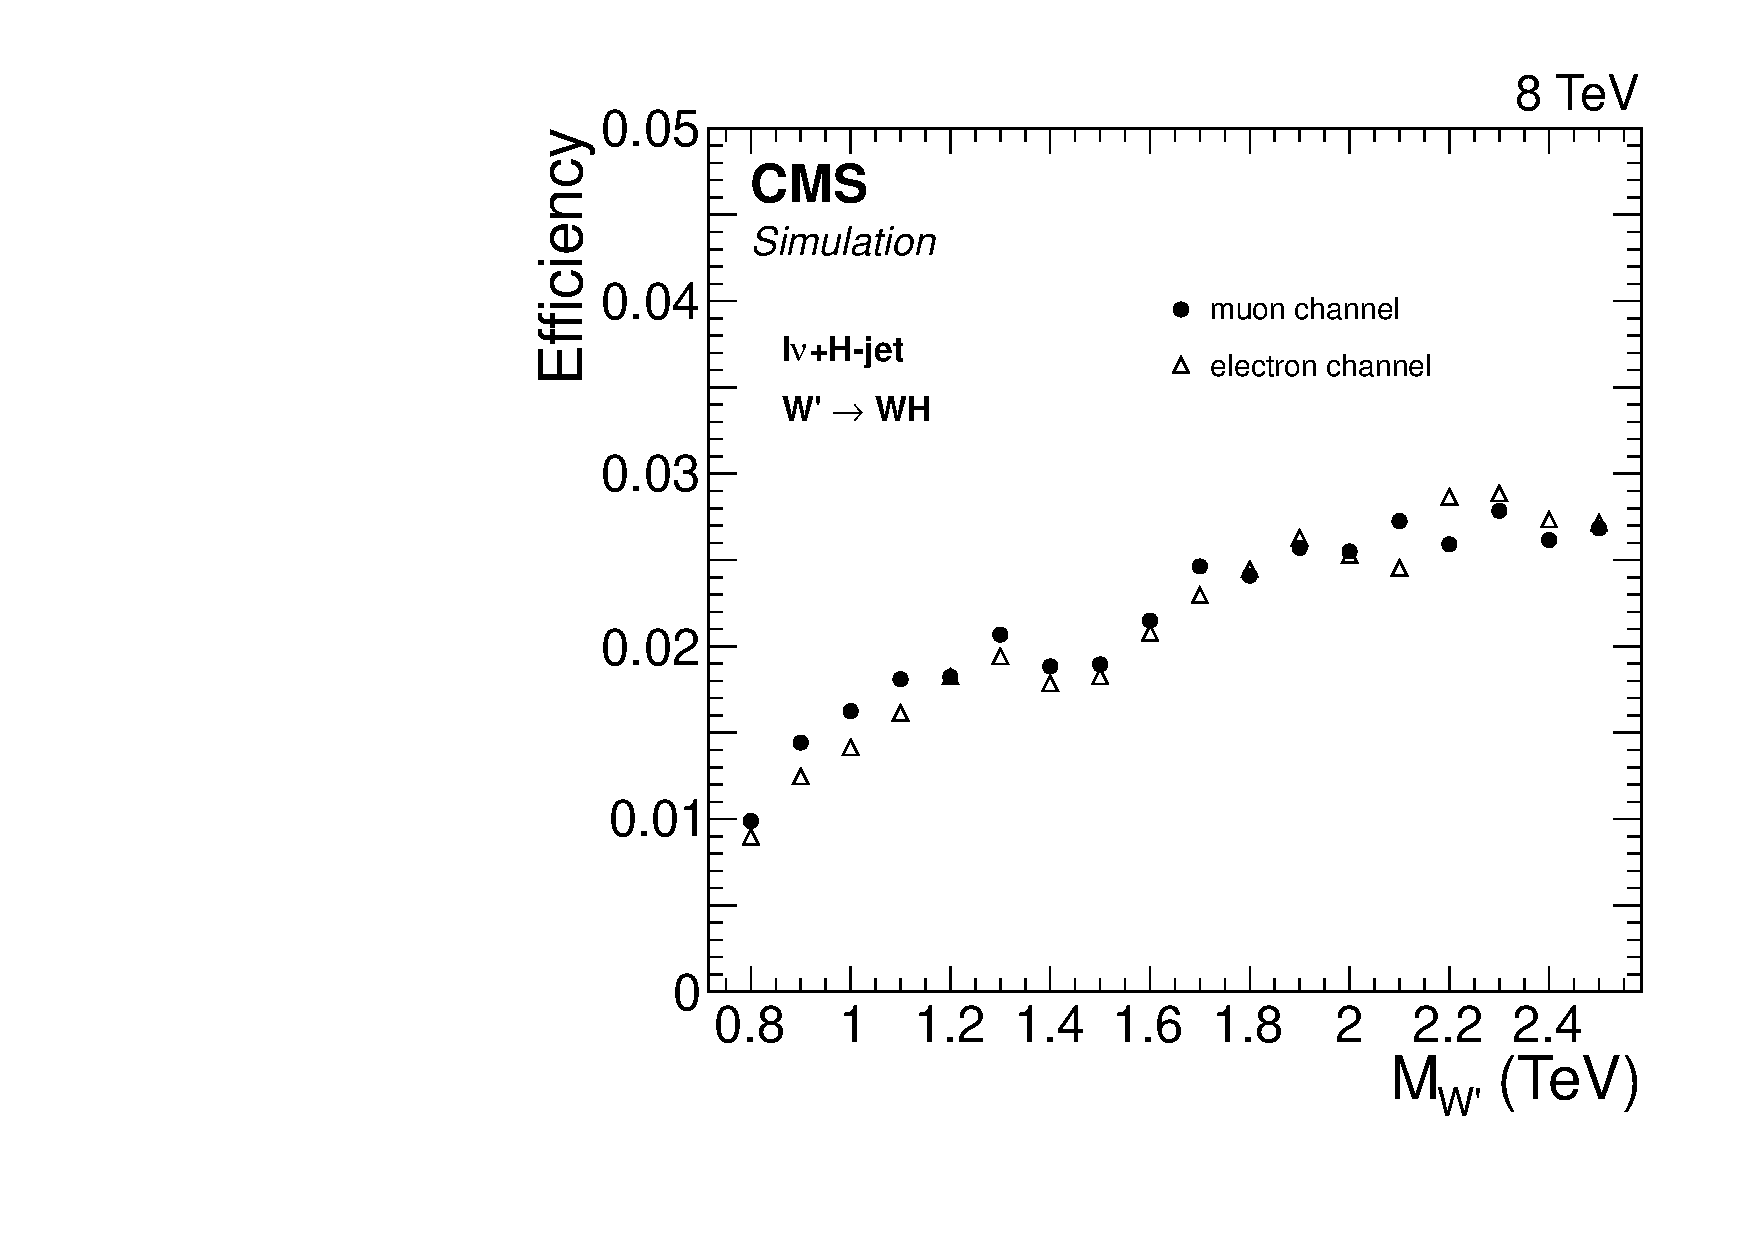
\includegraphics[width=0.3\textwidth]{\cheight/signal-eff-WH.pdf}
\caption{Signal efficiency in the $\ell\nu\bbbar$ analysis channel as a function of the generated \Wpr mass.}
\label{fig:effWH-8TeV}
\end{figure}
 
 %\section{Systematic uncertainties}\label{sec:systUnc}
 %%%%%%%%%
\section{Systematic uncertainties}\label{sec:systUnc}
%%%%%%%%%

This section describes the systematic uncertainties in the signal and background predictions affecting both the normalizations and the \mlvj distributions.
The uncertainties described below are included as nuisance parameters in the calculation of the limits on the cross section as well as of the p-values of potential excesses of events
observed in the data. %The uncertainties described below are all included as nuisance parameters in the statistic tool described in Section~\ref{sec:stat}.
%The systematic uncertainties in both background and signal predictions are described in Section~\ref{subsec:uncBkg} and ~\ref{subsec:uncSig}, respectively.

\subsection{Systematic uncertainties in the background estimation}\label{subsec:uncBkg}

The uncertainty in the W+jets background normalization is mainly due to the uncertainties in the parameters extracted from the fit of the data in the pruned-jet-mass sideband. This contribution is statistical in nature since it depends on the amount of data in the \mJ sideband regions, and it is evaluated varying the fit parameters from the final fit values by random amounts sampled from the covariance matrix.
Alternative parametrizations of the W+jets \mJ distribution have been studied and the differences with respect to the results obtained with the chosen default function taken into account by adding this effect in quadrature to the pure statistical contribution.
%An additional effect due to the difference arising from alternative parametrization of the W+jets \mJ distribution is taken into account and added in quadrature to the pure statistical contribution.
This contribution is found to constitute up to 15\% of the total uncertainty. The total uncertainty on the W+jets yields remains below 10\% in the $\ell\Pgn\qqbar$ channel, while uncertainties above 40\% are obtained for the $\ell\Pgn\bbbar$ channel where the amount of data in the sidebands is largely reduced by the tight b-tagging requirements.
%lv+jet
%mu HPW 5.1% - el HPW 7.3% - mu HPZ 8.4% - el HPZ 9.1%
%contribution from shape:
%mu HPW 0.5% - el HPW 0.06% - mu HPW 15% - el HPZ 3.3% 
%lv+Hjet
%mu 41.9% - el 59%

As described in Section~\ref{subsec:wjetshape} the extrapolated background shape in the signal region is computed from the product of $F_\mathrm{data, SB}^{\mathrm{W+jets}}$ and $\alpha_\mathrm{MC}$.
Thus, the shape uncertainty comes from both uncertainties in the W+jets \mlvj shape obtained from the fit of the data in the lower \mJ sideband region and in the modelling of the transfer function $\alpha_\mathrm{MC}$.
Both contributions are mainly statistical in nature, as they are driven by the available amount of data in the sideband and by the number of simulated W+jets events passing the analysis requirements, respectively.
%The first contribution depends on the amount of data in the lower sideband region and it is estimated from the covariance matrix of the fit.
These effects are estimated from the covariance matrix of the fit and included in the final limit and p-value calculations after a procedure which diagonalizes the matrix to decorrelate the fitted parameters.
In this procedure, the new parameters are defined in such a way to be centered at zero and with error equal to unity. The background fit parameterization is then redefined as a function of these new, uncorrelated parameters.
This new fit function together with the uncertainties in the fitted parameter is used to describe the background distribution in the limit and p-value calculations explained in Section~\ref{sec:stat}.

Additionally, the $\alpha_\mathrm{MC}$ (Fig.~\ref{fig:alphasWV_13TeV}) is affected by variations due to the choice of the parametrization used to model the W+jets distribution.
Previous studies showed that additional variations of about the same size are due to the use of different parton showering algorithms~\cite{Khachatryan:2014gha}. This effect has been evaluated comparing the $\alpha$ obtained with simulated samples with parton showering implemented through \HERWIG{++} and \PYTHIA{}. All these variations are found to be equal or slightly smaller than the statistical uncertainties on the $\alpha$, and hence the associated systematic effect is taken into account by enlarging the errors on the decorrelated fit parameters by a factor $\sqrt{2}$. This is sufficiently conservative to cover all the shape variations.
In a similar way, variations in the $F_\mathrm{data, SB}^{\mathrm{W+jets}}$ due to the same effects, are as well taken into account.

The uncertainties in the W+jets normalization are treated as uncorrelated among the different lepton flavor channels and $\mJ$ categories.
%, while the uncertainties in the W+jets distribution are partially correlated according to the following scheme:
While the uncertainties in the W+jets distribution are uncorrelated among electron and muon channels, a partial correlation among $\mJ$ categories is defined according to the following scheme:

\begin{itemize}
\item uncertainties in the $F_\mathrm{data, SB}^{\mathrm{W+jets}}$ parameters are correlated;
\item uncertainties in the $\alpha_\mathrm{MC}$ parameters are uncorrelated.
\end{itemize}

This solution takes into account the fact that in the different \mJ categories the same data in the sideband are used to estimate the W+jets distribution, while the transfer function is used to predict the shape in the two orthogonal signal regions defined by the categories.\\

The systematic uncertainty in the normalization of the \ttbar and single-top-quark backgrounds is driven by the uncertainties in the data-to-simulation scale factors estimated in the top-quark-enriched control sample (Section~\ref{sec:ttbar}). In the $\ell\Pgn\qqbar$ channel these uncertainties are measured to be 4.6\% and 8.4\% in the muon and electron channel, respectively. For the $\ell\Pgn\bbbar$ channel, this uncertainty amounts to 5.6\%.
%For the single top quark background an additional systematic uncertainty of 5\% in the NLO cross section calculation is assigned.
For the single-top-quark background an additional systematic uncertainty related to the cross section calculations is assigned to be 15\% and 5\%, for the 8 and 13\TeV data analysis respectively~\cite{Chatrchyan:2012ep,Kant:2014oha}.

The \ttbar background distribution in \mlvj is taken from simulation and this choice is found to be reasonable given the
agreement between data and simulation in the top-quark-enriched control sample (Fig.~\ref{fig:tt-mtop8TeV_a}).
However, previous studies~\cite{Khachatryan:2014gha} showed that variations in the shape occur due to the choices of regularization or factorization scales (varied up and down by a factor of 2),
to the matching scales in the \MADGRAPH{} simulation, and to different generators (\MADGRAPH{} or \POWHEG{}).
These effects are covered by enlarging the errors on the decorrelated fit parameters for the \ttbar distribution by a factor of 2.\\

The systematic uncertainties in the diboson background normalization is due to the uncertainty in the inclusive cross sections, which are assigned to be 10\%~\cite{Chatrchyan:2013oev} and 3\%~\cite{Gehrmann:2014fva} for the 8 and 13\TeV data analysis, respectively.
%EXO-14-010: The systematic uncertainties in the WW, WZ, and ZZ inclusive cross sections are assigned to be 10%, taken from the relative difference in the mean value between the CMS WW cross section measurement at $\sqrt{s} = 8\TeV$ and the SM expectation~\cite{www.arxiv.org/abs/1301.4698}.
%EXO-13-009 and Raffaele say 20% and cite same reference.
For the $\ell\Pgn\qqbar$ channel, the uncertainty in the diboson background normalization is as well due to the uncertainty of 3\% in the measured data-to-simulation scale factors for the V-tagging efficiency derived in the top-quark-enriched control sample (Section~\ref{sec:vtagging}).\\

Additional sources of systematic uncertainties in the background normalization are due to the uncertainty in the integrated luminosity, and in the measured data-to-simulation scale factors for the efficiency of lepton trigger and identification, described in the following section.

A summary of the systematic uncertainties in the normalization of the predicted background is provided in Tables~\ref{tab:uncBkg8TeV} and~\ref{tab:uncBkg13TeV} for the $\ell\nu\qqbar$ and $\ell\nu\bbbar$ analysis channel, respectively.

\begin{table}[!htb]
\begin{center}
\begin{tabular}{l|c|c|c|c}
Source                                       & W+jets & \ttbar  & Single top quark & Diboson \\
\hline
\hline
Integrated luminosity                 &             & 2.6\%  & 2.6\% & 2.6\% \\
Cross section                            & -           & -          & 15\%    & 10\% \\
Data-driven prediction               & 42\% ($\mu$) / 59\% (e) & 5.6\% & 5.6\% & - \\
Lepton trigger ($\mu$/e)            & -          & 1\% / 1\% & 1\% / 1\% & 1\% / 1\% \\
Lepton identification ($\mu$/e) & -           & 1\% / 3\% & 1\% / 3\% & 1\% / 3\% \\
\hline
\end{tabular}
\end{center}  
\caption{Summary of the systematic uncertainties in the normalization of the predicted background in the $\ell\Pgn\bbbar$ analysis at 8\TeV.}
\label{tab:uncBkg8TeV}
\end{table}

\begin{table}[!htb]
\begin{center}
\begin{tabular}{l|c|c|c|c}
Source                                       & W+jets & \ttbar  & Single top quark & Diboson \\
\hline
\hline
Integrated luminosity                 &             & 2.7\%  & 2.7\% & 2.7\% \\
Cross section                            & -           & -          & 5\%    & 3\% \\
V-tagging efficiency                   & -           & -          & -          & 3\% \\
Data-driven prediction               & 5--9\%  & 5--8\% & 5--8\% & - \\
Lepton trigger ($\mu$/e)            & -          & 1\% / 1\% & 1\% / 1\% & 1\% / 1\% \\
Lepton identification ($\mu$/e) & -           & 1\% / 3\% & 1\% / 3\% & 1\% / 3\% \\
\hline
\end{tabular}
\end{center}  
\caption{Summary of the systematic uncertainties in the normalization of the predicted background in the $\ell\Pgn\qqbar$ analysis at 13\TeV.}
\label{tab:uncBkg13TeV}
\end{table}

\subsection{Systematic uncertainties in the signal prediction}\label{subsec:uncSig}

Systematic uncertainties affecting the predicted signal efficiency (or normalization) and \mlvj distribution arise from several sources as described in the following and summarized in Tables~\ref{tab:sigUnc8TeV} and~\ref{tab:sigUnc13TeV}.
The effect of each source is evaluated for each considered simulated signal hypothesis as a function of the resonance mass.\\

%vtagging sf and mJ scale/resolution
One of the primary sources affecting the signal normalization for the $\ell\Pgn\qqbar$ channel is due to uncertainties in data-to-simulation scale factors for the V-tagging efficiency, derived from the top-quark-enriched control sample as described in Section~\ref{sec:vtagging}. These uncertainties include separately the uncertainty of 3\% on the scale factor measured in \ttbar events with an average \pt $\approx$ 200\GeV, and the uncertainty due to the extrapolation of the scale factor to higher momenta, which is assigned to be 6--10\% depending on the signal mass. Additional uncertainties are assigned due to the pruned-jet-mass scale and resolution measured in \ttbar events (Table~\ref{tab:Wmass13TeV}). These are computed by rescaling or smearing the \mJ value according to the uncertainties in the respective \mJ scale or resolution. The selection efficiencies are recalculated on these modified events, with the resulting changes taken as systematic uncertainties that depend on the resonance mass.

%htagging (btagging + mJ scale/resolution)
In a similar way, systematic uncertainties are assigned in the $\ell\Pgn\bbbar$ channel due to the uncertainty in the H-tagging efficiency.
This contribution arises from both uncertainties in the data-to-simulation scale factors for b-tagged jet identification efficiency (Section~\ref{subsec:bjets})
and for the efficiency of the \mJ selection for H jets.
The first is obtained by varying the b-tagging scale factors within the associated uncertainties and amounts to 2--8\% depending on the signal mass.
The second is evaluated by considering the uncertainties in the \mJ scale and resolution measured in \ttbar events for W jets,
additionally accounting for the difference in fragmentation of light quarks and b quarks, which amounts to 2.6\% (Section~\ref{sec:htagging}).
The systematic uncertainty in the mass tagging efficiency is found to be 2--10\%, depending on the signal mass.
%This contribution can be separated into two categories: the efficiency related to the b tagging and the efficiency related to the pruned H mass tag.
%This contribution arises from both uncertainties in the data-to-simulation scale factors for the pruned-jet-mass scale and resolution, derived from the top-quark-enriched control sample with 8\TeV data, and for b-tagged jet identification efficiencies (Section~\ref{subsec:bjets}). These sources introduce a systematic uncertainty in the mass tagging and b tagging of the Higgs boson of 2--10\% and 2--8\%, respectively, depending on the signal mass.\\
%The second is assumed to be similar to the mass selection efficiency of W jets estimated in Ref. [24], additionally accounting for the difference in fragmentation of light quarks and b quarks, which amounts to 2.6% per jet.

%jes/jer + lepton momentum/energy scale and resolution
The accuracy on energy and momentum measurements for leptons and jets represents an important source of systematic uncertainties in the signal efficiency.
In particular, the muon momentum scale and resolution, the electron energy scale and resolution, and the jet energy scale and resolution are considered.
The event selection is applied to the signal samples after varying the lepton four-momenta within one standard deviation of the corresponding uncertainty
in the muon momentum scale~\cite{Chatrchyan:2012xi} or electron energy scale~\cite{Chatrchyan:2013dga}, or applying an appropriate Gaussian momentum/energy smearing in case of resolution uncertainties.
The same procedure is also applied for the jet four-momenta using the corresponding energy scale and resolution uncertainties.
In this process, variations in the lepton and jet four-momenta are propagated consistently to the \ptvecmiss vector.
The signal efficiency is then recalculated using modified lepton and jet four-momenta separately for each source of systematic uncertainties.
The largest relative change in the signal efficiency compared to the default value is taken as the systematic uncertainty for that specific source.
The induced relative migration among V-jet mass categories is evaluated for the $\ell\Pgn\qqbar$ channel, but do not affect the overall signal efficiency. The muon, electron, and jet uncertainties are assumed to be uncorrelated. 
Finally, the resulting changes on the reconstructed resonances are propagated on the reconstructed \mlvj signal distribution, resulting in a small effect on both peak position and width of the Gaussian core.\\ 
%Raffaele: JES/JER 3% on the width - unclustered energy scale 1-3% on the width - lepton scales and resolutions < 1% on the peak - JES up to 1.5% on the peak
%EXO-13-009 same as Raffaele except: The uncertainty in the peak position of the signal is estimated to be less than 1%.
%WH: same as EXO-13-009
%WV 13TeV: JES mean 1.3% - JES width 2--3% - JER mean 0.1 - JER width 4%

%lepton trigger/identification 
The systematic uncertainties in the lepton trigger, identification, and isolation efficiencies are derived using a dedicated T\&P analysis in $\PZ\rightarrow\ell^+\ell^-$ events.
For both analysis channels, an uncertainty of 1\% is assigned to the trigger efficiency for both lepton flavors,
while for lepton identification and isolation efficiency, the systematic uncertainty is estimated to be 1\% for the muon and 3\% for electron flavors.\\

%lumi and PDFs
The 2.7\% and 2.6\% uncertainty in the integrated luminosity affects to the normalization of both signal and backgrounds in the $\ell\Pgn\qqbar$ and $\ell\Pgn\bbbar$ channel, respectively, as obtained in measurements performed for the 2015 and 2012 data taking periods~\cite{CMS-PAS-LUM-15-001,CMS:LUM13001}. 

For the $\ell\Pgn\qqbar$ channel, uncertainties on the signal yield due to variations in the parton distribution function and the choice of factorization ($\mu_{f}$) and renormalization ($\mu_{r}$) scales are also taken into account.
The PDF uncertainties are evaluated using the NNPDF 3.0~\cite{Ball:2011mu} PDF set.
The uncertainty related to the choice of $\mu_{f}$ and $\mu_{r}$ scales is evaluated following the proposal in Refs.~\cite{Cacciari:2003fi,Catani:2003zt} by varying the default choice of scales in the following 6 combinations of factors:
$(\mu_{f}$, $\mu_{r})$ $\times$ $(1/2, 1/2)$, $(1/2, 1)$, $(1,1/2)$, $(2, 2)$, $(2, 1)$, and $(1, 2)$.
The uncertainty in the signal cross section from the choice of PDFs and of factorization and renormalization scales ranges from 4 to 77\%, and from 1 to 22\%, respectively, depending on the resonance mass, particle type and its production mechanism.
For the $\ell\Pgn\bbbar$ channel, only the impact of the proton PDF uncertainties on the signal efficiency is evaluated with the PDF4LHC prescription~\cite{Botje:2011sn,Alekhin:2011sk}, using the MSTW2008~\cite{MSTW} and NNPDF 2.1~\cite{NNPDF} PDF sets. This effect is found to be $< 0.5\%$.

%pileup
Finllay, the systematic uncertainty due to the modelling of pileup is estimated by reweighting the signal simulation samples such that the distribution of the number of interactions per bunch crossing is shifted according to the uncertainty in the inelastic proton-proton cross section compared with that found in data. This contribution is found to be 0.5\% in both channels.
%btag veto
%An additional systematic, affecting the normalization of non data driven background, is repre-sented by the uncertainty in the data-to-simulation scale factors for b-jet identification, derived following [125].

\begin{table}[!htb]
\caption{Summary of the systematic uncertainties in the signal prediction for the $\ell\Pgn\bbbar$ analysis channel and their impact on the event yield in the signal region and on the reconstructed \mWH shape (mean and width) for both muon and electron channels.}
\centering
\begin{tabular}{lccc}
Source                                   & Relevant quantity          & Uncertainty (\%)\\
\hline
\hline
Lepton trigger ($\mu$/e) 	         & Signal yield		        & 1 / 1\\
Lepton identification	($\mu$/e)	& Signal yield		        & 1 / 3\\
Lepton \pt scale ($\mu$/e)         & Signal yield		        & 1 / 0.5\\
Lepton \pt resolution ($\mu$/e)  & Signal yield		        & 0.1 / 0.1\\
Jet energy scale                        & Signal yield		        & 1--3 \\
Jet energy resolution                 & Signal yield		        & 0.5 \\
Integrated luminosity		        & Signal yield		        & 2.6\\
Pileup                                        & Signal yield		        & 0.5\\
PDFs                                         & Signal yield		        & $<$ 0.5\\
H-jet mass tagging efficiency    & Signal yield 	                & 2--10\\
H-jet b-tagging efficiency          & Signal yield                    & 2--8\\
\hline
Jet energy scale		         & Resonance shape (mean)	 & 0.5\\
Jet energy scale		         & Resonance shape (width)	 & 4\\ 
Jet energy resolution	                 & Resonance shape (mean)	 & 0.2\\
Jet energy resolution		        & Resonance shape (width)	 & 4\\
Lepton \pt resolution                 & Resonance shape (mean)	 & 0.1\\
Lepton \pt resolution                 & Resonance shape (width)	 & 1.2\\
Lepton \pt scale                        & Resonance shape (mean)	 & 0.7\\
Lepton \pt scale                        & Resonance shape (width)	 & 2.5\\
\hline
\end{tabular}
\label{tab:sigUnc8TeV}
\end{table}

\begin{table}[!htb]
\caption{Summary of the systematic uncertainties in the signal prediction for the $\ell\Pgn\qqbar$ analysis and their impact on the event yield in the signal region and on the reconstructed \mWV shape (mean and width) for both muon and electron channels. The last uncertainty results in migrations between event categories, but does not affect the overall signal efficiency.}
\centering
\begin{tabular}{lccc}
Source                                   & Relevant quantity          & Uncertainty (\%)\\
\hline
\hline
Lepton trigger ($\mu$/e) 	         & Signal yield		        & 1 / 1\\
Lepton identification	($\mu$/e)	& Signal yield		        & 1 / 3\\
Lepton \pt scale ($\mu$/e)         & Signal yield		        & 0.7 / 0.2\\
Lepton \pt resolution ($\mu$/e)  & Signal yield		        & 0.1 / 0.1\\
Jet energy and \mJ{} scale        & Signal yield		        & 0.2--4 \\
Jet energy and \mJ{} resolution & Signal yield		        & 0.1--2 \\
Integrated luminosity		        & Signal yield		        & 2.7\\
Pileup                                        & Signal yield		        & 0.5\\
PDFs (\PWpr)                            & Signal yield		        & 4--19\\
PDFs (\PZpr)                             & Signal yield		        & 4--13\\
PDFs (\BulkG)                           & Signal yield		        & 9--77\\
$(\mu_{f}$ and $\mu_{r})$ scales (\PWpr)  & Signal yield & 1--14\\
$(\mu_{f}$ and $\mu_{r})$ scales (\PZpr)   & Signal yield & 1--13\\
$(\mu_{f}$ and $\mu_{r})$ scales (\BulkG) & Signal yield & 8--22\\
V-tagging efficiency                   & Signal yield 	                & 3\\
V-tagging \pt-dependence         & Signal yield                    & 6--10\\
\hline
Jet energy scale		         & Resonance shape (mean)	 & 1.3\\ 
Jet energy scale		         & Resonance shape (width)	 & 3\\ 
Jet energy resolution	                 & Resonance shape (mean)	 & 0.1\\
Jet energy resolution		        & Resonance shape (width)	 & 3\\
Lepton \pt resolution                 & Resonance shape (mean)	 & 0.1\\
Lepton \pt resolution                 & Resonance shape (width)	 & 0.1\\
Lepton \pt scale                        & Resonance shape (mean)	 & 0.1\\
Lepton \pt scale                        & Resonance shape (width)	 & 0.5\\
\hline
Jet energy and \mJ{} scale          & Migration                  & 2--24\\
\hline
\end{tabular}
\label{tab:sigUnc13TeV}
\end{table}

%\section{Testing new resonance hypothesis}\label{sec:stat}
 %%%%%%%%%
\section{Testing for a new resonance hypothesis}\label{sec:stat}
%%%%%%%%%

The purpose of this analysis is to infer a constraint on the existence of a new resonance decaying into diboson for a set of different signal mass hypotheses.
The comparison between the diboson invariant mass distribution observed in data and the SM background prediction is used to check for the presence of the new resonance.
A hypothesis test is built to decide between a null hypothesis given by the predicted SM background only, against an alternative hypothesis which includes both background as well as the sought after signal.
In principle one can either test the background-only hypothesis and exclude it if there is a large deviation of the data from the SM background prediction,
or test the signal hypothesis and exclude it if there is a large deviation of the data from the expected signal model.
In particular, if no significant deviation from the SM background prediction is observed in data, compatible with the signal hypothesis, an upper limit on 
production cross section of such signal is usually set, up to a certain degree of belief.
%From the statistical analysis of the reconstructed diboson invariant mass, one can infer that there is 95\% confidence level (CL) that the signal $\sigma\times\cal B$ is not larger than some value $?_\mathrm{95\%}$;
%otherwise, if the cross section was above this value, a statistically-significant excess of data would have emerged over the background.
%If the upper limit $?_\mathrm{95\%}$ is as large as the $\sigma\times\cal B$ predicted by some specific theoretical model $?_\mathrm{th}$ or smaller, it can be inferred that a resonance of that mass is excluded at 95\% C.L..
The CMS community has agreed upon a procedure for computing upper limits, which is based on the modified frequentist method, often referred to as $\mathrm{CL}_s$.
While a detailed description of this method can be found in Refs.~\cite{CLs1,Junk:1999kv}, the basic ingredients will be summarized Section~\ref{subsec:CLs}.
A description of the procedure followed to quantify an excess of events is provided in Section~\ref{subsec:pvalue}. A summary of the final results will be given in the next chapter.

\subsection{Limit setting procedure}~\label{subsec:CLs}

The procedure to establish the exclusion of a given signal hypothesis is based on a frequentist significance test which uses a log-likelihood ratio as a test statistic.
In order to construct the test statistic a likelihood function is defined as

\begin{equation}\label{eqn:likelihood}
{\cal L}( data | \mu,\theta) = \mathrm{Poisson}(data | \mu\cdot s(\theta) + b(\theta))\cdot p(\tilde{\theta}|\theta).
\end{equation}

In this definition, $s$ and $b$ denote the expected signal and background event yields, respectively,
which, before the scrutiny of the observed data entering the statistical analysis, are subject to multiple uncertainties that are treated by introducing nuisance parameters $\theta$,
so that signal and background expectations depend on these parameters as $s(\theta)$ and $b(\theta)$.
The exclusion of a signal hypothesis is generally expressed as an upper limit on the \textit{signal strength modifier} $\mu$
which scales the cross section used as input in the evaluation of the expected signal yields.
With this definition, the likelihood represents the Poisson probability of observing a certain amount of data when the expected yield is $\mu\cdot s(\theta) + b(\theta)$
and given the probability $p(\tilde{\theta}|\theta)$ of measuring a value $\tilde{\theta}$ for the nominal nuisance parameter $\theta$.
Note that, in this likelihood definition, ``data'' stands for a generic dataset, either experimental or a pseudo-data generated randomly.

The likelihood can be either binned or unbinned. In the first case the function $\mathrm{Poisson}(data | \mu\cdot s + b)$ in Eq.~\ref{eqn:likelihood} is the product of Poisson probabilities
for observing $n_i$ events in each bin $i$ of the signal+background model

\begin{equation}\label{eqn:binned}
\prod_i \frac{(\mu s_{i} +b_{i})^{n_i}}{n_i!}e^{-(\mu s_i + b_i)}.
\end{equation}

For the unbinned case each event enters the calculation as follows

\begin{equation}\label{eqn:unbinned}
k^{-1}\prod_i (\mu S f_s(x_i) + Bf_b(x_i))e^{-(\mu S + B)},
\end{equation}

\noindent where $k$ is the number of events, $f_s(x)$ and $f_b(x)$ are the probability density functions of signal and background of the observable $x$, while S and B are the total event rates expected for signal and background.
In this analysis the unbinned form for the likelihood is used, where the observable $x$ coincides with the reconstructed diboson invariant mass.\\

To compare the compatibility of the data with the background-only and signal+background hypotheses, where the prediction for the signal is allowed to be scaled by some factor $\mu$,
the test statistic $\tilde{q}_\mu$ is constructed based on the profile likelihood ratio as

\begin{equation}\label{eqn:testStatistic}
\tilde{q}_\mu = -2\ln\frac{{\cal L}(data | \mu,\hat{\theta}_\mu)}{{\cal L}( data | \hat{\mu},\hat{\theta})},\qquad \mathrm{with} \qquad 0 \leq \hat{\mu} \leq \mu.
\end{equation}

Here $\hat{\theta}_\mu$ denotes the value of $\theta$ that maximizes the likelihood for the hypothesized $\mu$,
i.e. it is the conditional maximum-likelihood (ML) estimator of $\theta$ (and thus is a function of $\mu$). 
The procedure of refitting the nuisance parameters to maximize the likelihood for each possible value of the parameter of interest $\mu$, is usually referred to as ``profiling''.
The denominator is the maximized (unconditional) likelihood function, i.e., $\hat{\mu}$ and $\hat{\theta}$ are the global maximum of the likelihood.
The presence of the nuisance parameters broadens the profile likelihood as a function of $\mu$ relative to what one would have if their values were fixed.
This reflects the loss of information about $\mu$ due to the systematic uncertainties.
Higher values of $\tilde{q}_\mu$ correspond to increasing incompatibility between the data and the hypothesized signal of strength $\mu$.
The lower constraint for $\hat{\mu}$ in the denominator excludes the possibility of negative signal yields. 
The upper constraint is introduced to avoid that data with $\hat{\mu} > \mu$ (upward fluctuations) are considered as representing less compatibility with $\mu$ than what obtained with data.

The observed value of the test statistic, $\tilde{q}_\mu^\mathrm{obs}$ for the given signal strength modifier $\mu$ under test is computed,
as well as the nuisance parameters $\hat{\theta}_0^\mathrm{obs}$ and $\hat{\theta}_\mu^\mathrm{obs}$ maximizing the likelihood under the background-only and signal+background hypothesis, respectively.
Furthermore, the probability density functions of the chosen test statistic $\tilde{q}_\mu$ under the signal+background hypothesis, $f(\tilde{q}_\mu|\mu,\hat{\theta}_\mu^\mathrm{obs})$,
and the background-only hypothesis, and $f(\tilde{q}_\mu|0,\hat{\theta}_0^\mathrm{obs})$, are constructed by means of ensembles of MC pseudo-experiments
generated according to the same Poisson probabilities used to build the likelihood. In this process the nuisance parameters 
are fixed to the values $\hat{\theta}_0^\mathrm{obs}$ and $\hat{\theta}_\mu^\mathrm{obs}$ obtained by fitting the observed data.

Using the $f(\tilde{q}_\mu|0,\hat{\theta}_0^\mathrm{obs})$ and $f(\tilde{q}_\mu|\mu,\hat{\theta}_\mu^\mathrm{obs})$ distributions,
two p-values are computed

\begin{equation}
\begin{gathered}
p_\mu \equiv \mathrm{CL}_{s+b} = P(\tilde{q}_\mu \geq \tilde{q}_\mu^\mathrm{obs}|\mu s(\hat{\theta}_\mu^\mathrm{obs}) + b(\hat{\theta}_\mu^\mathrm{obs})) = \int_{\tilde{q}_\mu^\mathrm{obs}}^{+\infty} f(\tilde{q}_\mu|\mu,\hat{\theta}_\mu^\mathrm{obs})d\tilde{q}_\mu \\
p_0 \equiv \mathrm{CL}_{b} = P(\tilde{q}_\mu \geq \tilde{q}_\mu^\mathrm{obs}|b(\hat{\theta}_0^\mathrm{obs})) = \int_{\tilde{q}_\mu^\mathrm{obs}}^{+\infty} f(\tilde{q}_\mu|0,\hat{\theta}_0^\mathrm{obs})d\tilde{q}_\mu.
\end{gathered}
\label{eqn:pvalues}
\end{equation}

The two probabilities are shown in the example in Fig.~\ref{fig:CLs-ex_a}.
In the classical frequentist approach, the level of agreement between the data and hypothesized $\mu$ is evaluated by using the $\mathrm{CL}_{s+b}$ probability only,
and one says that the hypothesized signal $\mu$ is excluded at 95\% CL if $\mathrm{CL}_{s+b} \leq 0.05$.

However, such a definition has a caveat. If the distributions of the test statistic for the signal+background and background-only hypotheses have a not negligible overlap as in the plot (c) of Fig.~\ref{fig:CLs-ex_b},
the experiment would tend to exclude the hypothesized signal $\mu$ even if the experiment in this case has little sensitivity to discriminate it against the background.
In fact, in this case the experimental data are highly contaminated with background and a statement about the signal would be a mistake of interpretation.
To prevent the inference of a signal in such cases, the so-called modified frequentist approach has been introduced at the time of LEP~\cite{CLs1,Junk:1999kv}.
In this approach, the level of agreement between the data and hypothesized $\mu$ is evaluated by using instead the quantity 

\begin{equation}
\mathrm{CL}_s = \frac{\mathrm{CL}_{s+b}}{\mathrm{CL}_b},
\end{equation}

and the hypothesized signal $\mu$ is excluded at 95\% confidence level (CL) if $\mathrm{CL}_s \leq 0.05$.
It is straightforward to see from plot (a) of Fig.~\ref{fig:CLs-ex_b} that, if the distribution of the test statistic for the signal+background hypothesis
is well separated from the background-only distribution, then $\mathrm{CL}_s \sim \mathrm{CL}_{s+b}$ and there is no risk of misinterpretation.

In order to quote, as conventionally done, 95\% CL observed upper limits, the full procedure is iterated for different values of $\mu$, until $\mathrm{CL}_s = 0.05$ is found.
This value of $\mu$ is denoted as $\mu_{95\%}$, and one can infer that the hypothesized resonance X$\rightarrow$WV/VH with a cross section $\mu$-times larger than the one predicted 
by some specific theoretical model $\sigma_{th}$ used as input to the statistical analysis, is excluded at 95\% CL.
In this analysis, model-independent limits on the cross section are set by rescaling the $\mu^{95\%} = \sigma_{95\%}/\sigma_{th}$ by the input cross section in order to obtain $\sigma_{95\%}$.

\begin{figure}[!htb]
\centering
\subfigure[]{\label{fig:CLs-ex_a}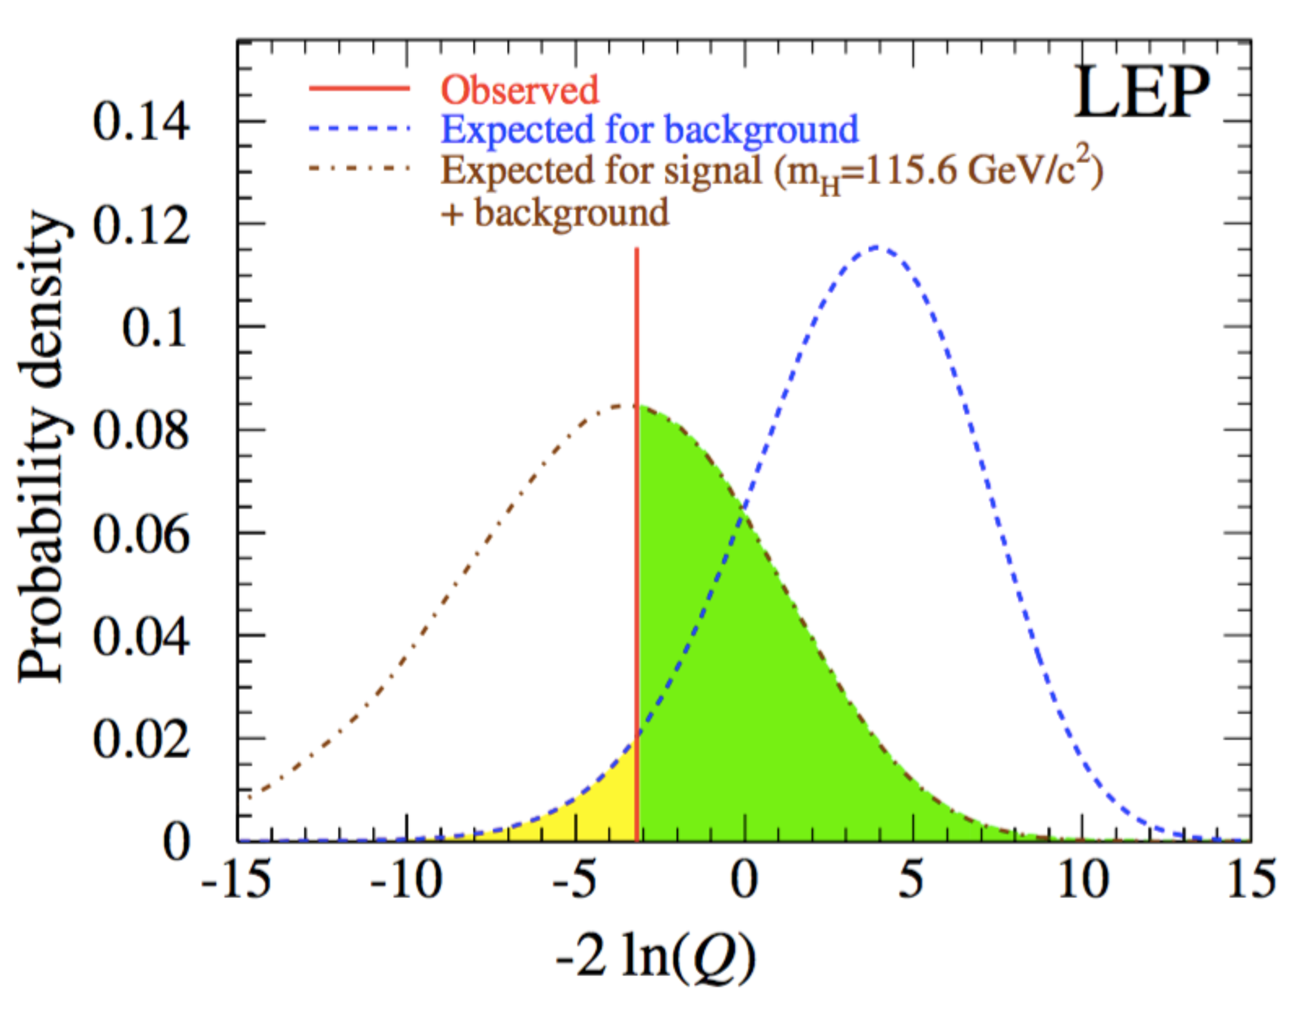
\includegraphics[width=0.55\textwidth]{\cheight/CLs_fig1.pdf}}
\subfigure[]{\label{fig:CLs-ex_b}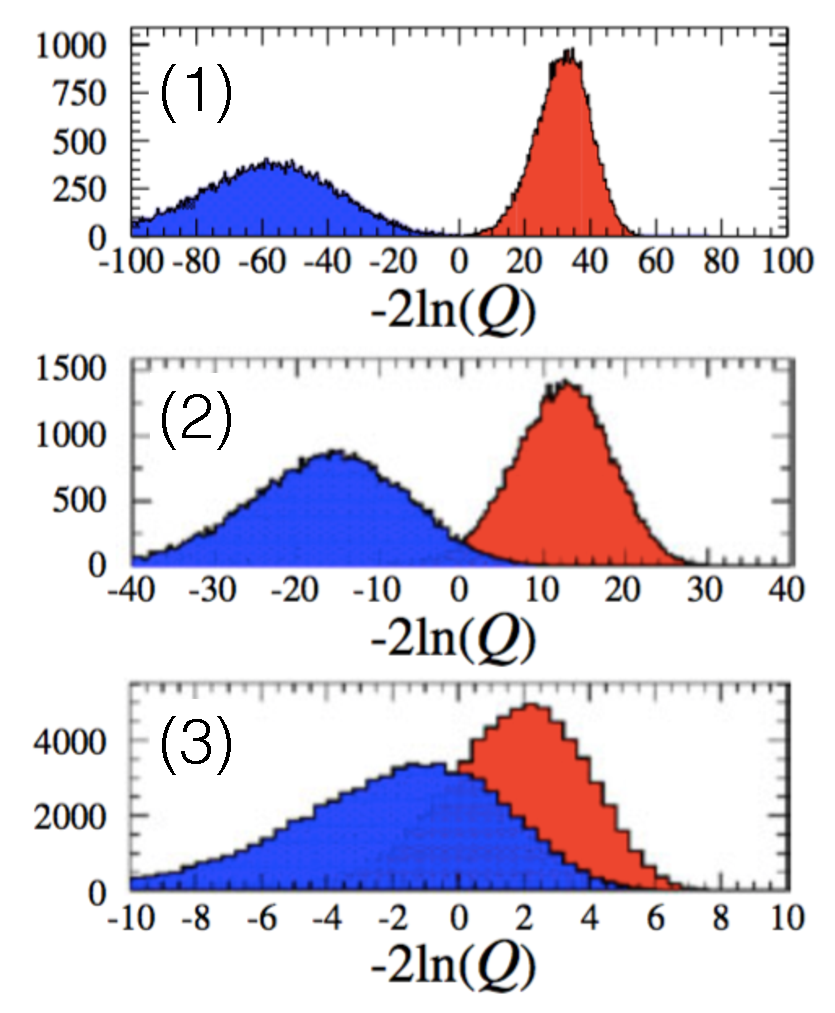
\includegraphics[width=0.35\textwidth]{\cheight/CLs_fig2-1.pdf}}
\caption{(a) Distributions of the test statistic $Q$ (defined in the text as $\tilde{q}_\mu$) for the combined Higgs search at LEP for the background (right) and signal+background hypotheses (left) for $m_\PH = 115.6\GeV$.
The light grey region to the left of the observation is $1-\mathrm{CL}_b$ and the dark grey region to the right of the observation is $\mathrm{CL}_{s+b}$. (b) Illustration of the evolution of the test statistic distributions with falling search sensitivity from (1) to (3)~\cite{CLs1}.}
\label{fig:CLs-ex}
\end{figure}

In addition to the observed upper limit derived from the actual data distribution, it is important to study also the expected limit given the observed data.
In fact, the expected limit quantifies the sensitivity of the experiment independent from statistical fluctuations in the data.
%The expected $\mathrm{CL}_s$ is extracted by computing the p-values of Equation~\ref{eqn:pvalues} using the median of the 
%$f(\tilde{q}_\mu|0,\hat{\theta}_0^\mathrm{obs})$ distribution instead of the observed value of the test statistic $\tilde{q}_\mu^\mathrm{obs}$.
%In this way a limit is extracted under the assumption that the data lies at the center of the expectation for the background-only hypothesis.
%In addition to the expected limit one can also extract the variation of the expected limit within the uncertainties.
%By using the values of the 16\% (2.5\%) and 84\% (97.7\%) quantiles of the $f(\tilde{q}_\mu|0,\hat{\theta}_0^\mathrm{obs})$,
%instead of the median, the $\pm 1(2)\sigma$ uncertainty bands are obtained.
In order to compute the median-expected upper limit, and the associated $\pm 1\sigma$ and $\pm 2\sigma$ bands,
a large set of background-only pseudo-experiments is generated and, for each of them, the $\mu_{95\%}$ is calculated.
From the cumulative distribution of $\mu_{95\%}$, the median value is taken as the expected limit, while the $\pm 1(2)\sigma$ uncertainty bands on the expected limits
are extracted from the values of the 16\% (2.5\%) and 84\% (97.5\%) quantiles.

\subsection{The asymptotic approximation}\label{subsec:AsymptCLs}

In order to compute $\mathrm{CL}_s$ the probability density functions of the test statistics are required.
In particular, one needs the probability density functions $f(\tilde{q}_\mu|\mu^\prime)$, where $\mu^\prime = 0$ or $\mu^\prime = \mu$,
which are obtained from MC pseudo-experiments requiring very expensive computational resources.
An approximation for the $\mathrm{CL}_s$ method, valid in the large sample limit, also referred to as ``asymptotic approximation'' has been proposed in Ref.~\cite{AsymptCLs}
and it is briefly described in the following.\\

By using the Wald approximation~\cite{10.2307/1990256} the desired distribution $f(\tilde{q}_\mu|\mu^\prime)$ can be obtained by expressing the test statistic given by the log-likelihood ratio as

\begin{equation}
\tilde{q}_\mu = \frac{(\mu-\hat{\mu})^2}{\sigma^2} + \mathcal{O}(1/\sqrt{N}),
\end{equation}

where $\hat{\mu}$ follows a Gaussian distribution with a mean $\mu^\prime$ and standard deviation $\sigma$, and $N$ represents the data sample size.
For large data samples ($N\rightarrow\infty$), the $\mathcal{O}(1/\sqrt{N})$ can be neglected and it can be shown~\cite{wilks1938} that the distribution $f(\tilde{q}_\mu|\mu^\prime)$ of the test statistic $\tilde{q}_\mu$
follows a \textit{noncentral chi-square} distribution for one degree of freedom with noncentrality parameter

\begin{equation}
\Lambda = \frac{(\mu-\mu^\prime)^2}{\sigma^2}.
\end{equation}

For the special case $\mu^\prime = \mu$ one has $\Lambda = 0$ and the test statistic is distributed as a chi-square for one degree of freedom.
For the general case in which $\mu^\prime \neq \mu$, the standard deviation $\sigma$ of $\hat{\mu}$ has to be evaluated, which depends on the MLE estimator of the nominal nuisance parameters.
The evaluation of $\sigma$ is greatly simplified considering a special, artificial data set, referred to as the ``Asimov data set'', where all statistical fluctuations are suppressed and the estimators for all parameters
are replaced by their expectation values as follows:

\begin{equation}
\hat{\mu} = \mu^\prime \qquad\qquad \mathrm{and} \qquad\qquad \hat{\theta} = \theta.
\end{equation}

With these assumptions the test statistic $\tilde{q}_{\mu,A}$ for the Asimov dataset is given by 

\begin{equation}
\tilde{q}_{\mu,A} \approx \frac{(\mu-\mu^\prime)^2}{\sigma^2} = \Lambda.
\end{equation}

From the Asimov data set one therefore obtains an estimate of the noncentrality parameter $\Lambda$ that characterizes the distribution $f(\tilde{q}_\mu|\mu^\prime)$.
Equivalently, the above equation can be used to obtain the variance $\sigma^2$ which characterizes the distribution of $\hat{\mu}$, namely,

\begin{equation}
\sigma_A^2 = \frac{(\mu-\mu^\prime)^2}{\tilde{q}_{\mu,A}},
\end{equation}

so that the distribution obtained by using $\sigma_A^2$ has a median given by the corresponding Asimov value $\tilde{q}_{\mu,A}$. 
Using these formulae, asymptotic relations are derived which are easily solved for the observed upper limits with the $\mathrm{CL}_s$ method,
as well as for the expected median and error bands.

\subsection{Quantifying an excess of events}~\label{subsec:pvalue}

The presence of the signal is quantified by the background-only p-value, i.e. the probability for the background to fluctuate
and give an excess of events as large or larger than the observed one.
As for the upper limits, this evaluation requires defining a test statistic and the construction of its probability density function.
For a given resonance mass hypothesis $M_X$, the test statistic used in this case is $\tilde{q}_0$, defined as

\begin{equation}
\tilde{q}_0 = -2\ln\frac{{\cal L}(data | 0,\hat{\theta}_0)}{{\cal L}( data | \hat{\mu},\hat{\theta})},\qquad \mathrm{with} \qquad \hat{\mu} \geq 0.
\end{equation}

%The constraint $\hat{\mu} \geq 0$ gives an accumulation of the test statistic at zero for events with downward fluctuations, since we are not interested in interpreting a deficit of events with respect to the expected background on an equal footing with an excess.
The probability density function $f(\tilde{q}_0|0,\hat{\theta}_0^{obs})$ is built by generating MC pseudo-experiments under the assumption of the background-only hypothesis.
From this distribution, the p-value corresponding to a given experimental observation $q_0^{obs}$ is evaluated:

\begin{equation}
p_0 = P(\tilde{q}_0 \geq \tilde{q}_0^\mathrm{obs}|b(\hat{\theta}_0^\mathrm{obs})) = \int_{\tilde{q}_0^\mathrm{obs}}^{+\infty} f(\tilde{q}_0|0,\hat{\theta}_0^\mathrm{obs})d\tilde{q}_0.
\end{equation}

This probability is converted into a \textit{significance}, also referred to as \textit{Z value}, as follows

\begin{equation}
Z = \Phi^{-1} (1-p_0).
\end{equation}

A significance of 5$\sigma$, corresponding to a p-value of 2.87$\times$10$^{-7}$, is conventionally used in high energy physics to claim a discovery,
and 3$\sigma$ for an evidence.

It can be demonstrated that in the asymptotic approximation (Section~\ref{subsec:AsymptCLs}), the likelihood ratio test statistic $\tilde{q}_0$
follows a chi-square distribution for one degree of freedom, and a fair estimate of the p-value and of the significance can be obtained from the observed value $\tilde{q}_0^\mathrm{obs}$ itself,
without the need for generating pseudo-data, as follows

\begin{equation}
\begin{gathered}
p_0 = \frac{1}{2} [ 1 - \mathrm{erf}(\sqrt{\tilde{q}_0^\mathrm{obs}/2}) ] \\
Z = \sqrt{\tilde{q}_0^\mathrm{obs}}.
\end{gathered}
\end{equation}

%\sqrt{\tilde{q}_0^\mathrm{obs}/2}
The p-value discussed above is evaluated at a fixed resonance mass $M_X$ and can be referred to as a \textit{local p-value}.
In this search, a scan is performed over a wide range of resonance mass hypotheses with the aim of finding
the minimum local p-value, which describes the probability of a background fluctuation for that particular resonance mass hypothesis.
However, it is important to distinguish the probability of finding a fluctuation in some particular location from the probability of finding such a fluctuation anywhere else in the spectrum.
The former is associated to the so called \textit{local significance}, whereas the latter is referred to as the \textit{global significance}.
The fact that the global significance is usually smaller than the largest local one is often referred to as the ``look-elsewhere effect'' (LEE).
As demonstrated in Ref.~\cite{Gross:2010qma}, the global and local p-values are related to each other by a multiplicative factor, usually referred to as ``trial factor'', proportional to the number of independent search regions.
In the asymptotic approximation the trial factor grows linearly with the local significance, through a proportional constant
that is related to the ratio between the mass range under consideration divided by its resolution. In particular, it can be shown that

\begin{equation}\label{eqn:trials}
trial\# = \frac{p_{global}}{p_{local}} \approx \frac{1}{3}\frac{mass\ range}{mass\ resolution}Z_{local}.
\end{equation}

The trial factor is best estimated through MC methods as it will be shown in Section~\ref{sec:signif8TeV}. However, a good agreement with the equation above is obtained.